%
%  Main file for James Till Matta's dissertation
%
%%%%%%%%%%%%%%%%%%%%%%%%%%%%%%%%%%%%%%%%%%%%%%%%%%%%%%%%%%%%%%%%%%%%%%%%

\documentclass[final,numrefs,sort&compress]{nddiss2e}

\usepackage{graphicx}   % need for figures
\usepackage{dcolumn}    % use to align table columns on decimal point
\usepackage{epstopdf}   % allows use of eps figures
\epstopdfsetup{update}  % only regenerate pdf files when eps file is newer
%\usepackage{xstring}    % for \IfEqCase
\usepackage{amssymb}    % for a few symbols
\usepackage{multirow}   % for the multirow command
\usepackage{booktabs}   % for nice lines in tables
\usepackage{longtable}  % for super long tables (I'm looking at you calibration parameter sets)
\usepackage{xfrac}      % for sfrac
\usepackage{braket}     % for good looking bra-ket notation
\usepackage{mathrsfs}   % for math script symbols like those used for rotation operators
\usepackage{ dsfont }   % for fancy integer symbols
\usepackage{ragged2e}
% % % % % % % % % % % % % % % % % %
% Define a few commands for conveniences sake
\newcommand{\gr}{$\gamma$ ray}
\newcommand{\pr}{$^{135}$Pr}
\newcommand{\uvec}[1]{\boldsymbol{\hat{\textbf{#1}}}}


\begin{document}

\frontmatter 
\title{EXOTIC NUCLEAR EXCITATIONS:\\
THE TRANSVERSE WOBBLING MODE IN \pr{}}
\author{James Till Matta}
\work{Dissertation}
\degaward{Doctor of Philosophy}
\advisor{Umesh Garg}
\department{Physics}

\maketitle
%%%%%%%%%%%%%%%%%%%%%%%%%%%%%%%%%%%%%%%%%%%%%%%%%%%%%%%%%%%%%%%%%%%%%%%%
%
% Front stuff
%
%%%%%%%%%%%%%%%%%%%%%%%%%%%%%%%%%%%%%%%%%%%%%%%%%%%%%%%%%%%%%%%%%%%%%%%%

% You must either set the copyright information or put your work in the public domain.
\copyrightholder{James Till Matta} % See template or documentation for
\copyrightyear{2015}           % other copyright options.
\makecopyright

% An abstract is optional for a mster's thesis, and required for a doctoral dissertation.
\begin{abstract}
The exotic collective excitation transverse wobbling has been investigated in the nucleus, \pr{}. A pair of zero and one-phonon wobbling bands has been observed. The nature of these wobbling bands was confirmed by the $\Delta{}I=1, E2$ nature of the $n_w=1\rightarrow n_w=0$ interband transitions making \pr{} the first nucleus observed to exhibit wobbling behavior other than five nuclei in the $A\sim{}160$. Additionally, a possible two-phonon wobbling band has been observed and its nature has been partially confirmed by measuring the $\Delta{}I=1, E2$ nature of the $n_w=2\rightarrow n_w=1$ interband transitions. The theory of transverse wobbling was proposed to explain contradictions in the wobbling energy predicted by previous quasiparticle plus triaxial rotor calculations; this theory has been confirmed. In this model, the quasiparticle aligns with an axis perpendicular to the axis with maximal moment of inertia (in contrast to previous theories, which aligned the quasiparticle with the axis with maximum moment of inertia). With this modification the fall in the energy of the wobbling phonon, observed in experiment, is now correctly predicted by theory. This confirmation of theory suggests a reevaluation of the previously discovered wobbling nuclei in the $A\sim{}160$ region in the framework of transverse wobbling as well.
\end{abstract}

% A dedication is optional.
\renewcommand{\dedicationname}{DEDICATION:}

\begin{dedication}
	To my fianc\'e Tina.\\\&\\To my parents, James and Margaret.\\
	In loving recognition of their support.
\end{dedication}

% These are required, and must be in this order.
\tableofcontents
\listoffigures
\listoftables

\begin{acknowledge}
In the long and difficult period I have been a student at Notre Dame many individuals have assisted me, giving their time, scientific guidance, and emotional support, without them I would have failed in this task and I remain indebted to them. I would like to sincerely thank every contributor to this work; thank you.

Foremost, I would like to offer my most profound thanks to Dr. Umesh Garg, my research advisor here at Notre Dame. I am grateful for his introducing me to the world of nuclear physics. Without his guidance, none of this would have been possible. Without his understanding, I would not have succeeded. His push to constantly improve my analysis and test \emph{why} something happens rather than simply accept it has had a major impact on me and my way of thinking. Without his patience, comments, and advice, this manuscript would be much poorer. I am profoundly gratefule for his advice and assistance.

I would like to thank my committee, past and present, for their assistance and advice. To Dr. James Kolata and Dr. Collin Jessop, I would like to apologize for the scheduling problems that prevented your participation in the defense, and accept my sincere thanks for steering my research and giving good advice on post-doctorate positions. Dr. Stefan Frauendorf's assistance has been invaluable in helping me understand the theory behind this work; I remain in your debt. To Dr. Anna Simon and Dr. Bruce Bunker, your willingness to become members of my committee on short notice has enabled me to complete this effort. You have my deepest thanks and gratitude.

I would like to extend thanks to Ms. Weichaun Li, Dr. Friedrich D\"onau, and Dr. Stefan Frauendorf for their excellent theoretical work. It has made a more complete interpretation and understanding of the data possible.

To Dr. Rajarshi Raut I extend my humble thanks. His patience with my many questions was genuinely appreciated. Equally appreciated was his guidance in a land that was new and different to me.

I would like to thank Dr. Robert V.F. Janssens, without his assistance, guidance, and patience in early conferences, I would have been lost.

What skills I have learned in the analysis and interpretation of gamma-ray coincidence data, I owe to Dr. Somsundar Mukhopadhyay, Dr. Shaofei Zhu, Dr. Xiaofeng Wang, and Dr. Daryl Hartley. The codes they provided and the skills they taught are a great boon to me, and I am thankful for their patience in passing them on.

I would like to deeply thank Dr. Akaa D. Ayangeakaa and Dr. Darshana Patel. They were my year-mates and friends while here. Their counsel has assisted me in maturing and their scientific discussions have enlightened. Further, their camaraderie has made for pleasant times while at Notre Dame. I thank you both from the bottom of my heart.

I would like to thank the other scientists who collaborated on the work presented in this dissertation Dr. Rudrajyoti Palit, Dr. Sudipta Saha, Dr. Jasmine Sethi, Dr. Tarkeshwar Trivedi, Dr. Sandeep S Ghugre, Dr. Ajit K Sinha, Dr. Michael P. Carpenter, Dr. Torben Lauritsen, Dr. Darek Seweryniak, Dr. Filip Kondev, Dr. Christopher J. Chiara, Ms. D. Vijaya Lakshmi,  Dr. P.V. Madhusudhana Rao, Dr. M. Kumar Raju, Dr. Sujit Tandel, and Dr. Sudipta Ray. Without their support in sitting shifts and dealing with the data, this task would have been Herculean at best and impossible, more realistically.

I wish to thank the staff of the ATLAS facility and the TIFR-BARC Pelletron facility. Without their diligent troubleshooting and operation of the machines, this journey could not have started, let alone finished.

If in my haste, I have omitted anyone I offer my sincere apology. So many have been of assistance in this quest; I am profoundly moved by their generosity of spirit.

I would like to thank my parents Margaret and James. Without their anecdotes of their own time in graduate school, I would be much less sane. Without their copy editing, this document would be poorer, and rife with grammatical errors.

Last but most important, I would like to thank my fianc\'{e} Tina without her, love, understanding, and emotional support I would have fallen from this path long ago.

This work has been supported in part by the U.S. National Science Foundation [Grants No. PHY-0758100 (UND), PHY-1068192 (UND), PHY-1419765(UND), and No. PHY-1203100 (USNA)]; by the APS-IUSSTF Physics Student and Post-doc Visitation Program; by the U.S. Department of Energy, Office of Science, Office of Nuclear  Physics,  under  Contracts  No.  DE-AC02-06CH11357 (ANL), No. DE-FG02-95ER40934 (UND), and No. DE-FG02-94ER40834 (UMCP); and by the Department of Science and Technology, Government of India (Grants No. IR/S2/PF-03/2003-II and No. IR/S2/PF-03/2003-III). This research used resources of ANL’s ATLAS facility, which is a DOE Office of Science User Facility.
\end{acknowledge}

% A symbols section is optional.
\begin{symbols}
\sym{c}{Speed of light in vacuum}
\sym{\hbar}{Reduced Planck Constant}
\sym{FWHM}{Full Width at Half Maximum}
\sym{Z}{Number of protons within a nucleus}
\sym{A}{Number of nucleons within a nucleus}
\sym{pnA}{particle nanoamps ($6.24151\times{}10^9$ particles/second)}
\end{symbols}

\mainmatter
%
% An unnumbered chapter (features)
%
%\unnumchapter{FEATURES OF FORMATTING IN THIS EXAMPLE FILE}
% The \unnumchapter command allows you to include an unnumbered chapter as part of
% the main text before Chapter 1. It will appear in your table of contents, and you
% should have at most one such chapter (although nothing in the class file will
% prevent you from creating more).

%
% Chapter 1 - General Introduction
%
%
%  Chapter:  1 - Introduction
%  Modified: 2/16/2015
%  Author:   James Till Matta
%
%%%%%%%%%%%%%%%%%%%%%%%%%%%%%%%%%%%%%%%%%%%%%%%%%%%%%%%%%%

\chapter{INTRODUCTION}
\label{chp:intro}
\section{Rotation of Deformed Nuclei}
\label{sec:intro-rot-def-nuc}
Rotation is a universal phenomenon. It exists in the macroscopic world where objects can rotate independently about any set of axes. In the microscopic world of quantum mechanics the situation is more complicated. Rotation about an axis of symmetry is forbidden as the wave function is unchanged. Thus rotation must be about an axes that are not axes of symmetry, limiting it to objects that are deformed, \emph{i.e.} not spherical.

\subsection{Axial Deformation}
\label{ssec:intro-rot-axial-def}
Spherical nuclei are in many ways, exceptional, as Fig. \ref{fig:chp1-quad-def} shows, deformation occurs in many regions of the nuclear chart. In most cases the deformation is slight enough that spherical models can be employed to describe most nuclear properties. However there are regions of the nuclear chart where the deformation grows large enough that it can no longer be ignored. Examples of these regions are the $A\sim{}130$ region and the $A\sim{}170$ region.

\begin{figure}[t!]
\centerline{\includegraphics[width=\textwidth,clip=true,trim=0 0 0 75]{./img/c1/chart_thb2.pdf}}
	\caption{Quadrupole deformation parameter $\beta_2$ across the nuclear chart. Plot adapted from \cite{nilssonDiagrams} which used data from \cite{mollerGroundStateDef}.\label{fig:chp1-quad-def}}
\end{figure}

While axial symmetry includes both oblate (pumpkin shaped) and prolate (cigar like) shapes there are quite few oblate nuclei, the majority have prolate deformation. This is usually understood as an effect of single particle structure from the Nilsson model (the Nilsson model is discussed in more detail in Chapter 2). Overall, prolate deformation moves more orbitals to low energy than oblate deformation, therefore in situations where there are several particles a sum over these particles will favor prolate shapes.

\subsection{Triaxiality}
\label{ssec:intro-rot-triax}
Nuclear triaxiality has been a subject of interest for years. While most deformed nuclei are axial in their shape, triaxial shapes have been predicted at low to moderate spin for a few regions of the nuclear chart, \emph{e.g.} Z=60, N=76 and Z=46, N=66  \cite{groundStateTriax}. In searching for triaxiality we are aided by the existence of two unique fingerprints, chirality and wobbling, phenomena that cannot exist unless the nuclear shape is triaxial.

\subsubsection{Chirality}
\label{sssec:intro-rot-chiral}
First predicted in 1997  by S. Frauendorf and J. Meng, chirality occurs when the axis of rotation lies outside the plains spanned by the principal axes of the nucleus \cite{frauendorfChirality,chiralityOfNuclearRotation,frauendorfTAC}. In this configuration the three axes of the nucleus form a screw with respect to the angular momentum vector allowing the construction of two orthogonal configurations with left and right-handed chirality. This manifests itself as pair of nearly degenerate $\Delta{}I=1$ bands with the same parity. Experiment has confirmed the existence of pairs of chiral bands in the $A\sim{}190$, $A\sim{}130$, $A\sim{}100$, and  $A\sim{}80$ regions of the chart of the isotopes, an example from each mass region can be found in Refs. \cite{chiralityMore135Nd,chiralityIn104Rh,chiralityIn188Ir,chiralityIn80Br}

\subsubsection{Wobbling}
\label{sssec:intro-rot-wob}
Of the two fingerprints of nuclear triaxiality, nuclear wobbling was perhaps the longest anticipated. First predicted by A. Bohr and B. Mottelson in Ref. \cite{bohrMottelson2}, wobbling was not observed until the work in 2001 by \O{}deg\aa{}rd \emph{et al.} \cite{wobblingIn163Lu}. Later four more wobbling nuclei were discovered expanding the list to $^{161,163,165,167}$Lu and $^{167}$Ta \cite{wobblingIn163Lu,wobblingIn163LuTwoPhonon,wobblingIn165Lu,wobblingIn167Lu,wobblingIn161Lu,wobblingIn167Ta}. In the wobbling mode is the quantum mechanical analog of the spinning motion of an asymmetric top. In the high spin limit, where most of the spin is aligned along a principle axis, the wobbling mode is a harmonic vibration describing the precession and nutation of a principal axis of the nucleus about the angular momentum vector.

\subsection{Motivation}
\label{ssec:intro-rot-motivation}
Problematically, while theory predicts an increase for the experimental wobbling energy, given by:
\begin{equation}
\Delta{}E=\hbar\omega_w(I)=E(I,n_w=1)-(E(I-1,n=0)+E(I+1,n_w=0))/2
\end{equation}
to increase with increasing angular momentum, the observed effect is a decrease (see Fig. \ref{fig:chp1-wobbling-freq}). S. Frauendorf and F. D\"{}onau solved this problem with their modified wobbling mode known as ``transverse'' wobbling \cite{frauendorfTransverseWobbling}. Contrary to previous models where the quasiparticle was coupled to the intermediate axis (called ``longitudinal wobbling''), see, for example, Refs. \cite{oldQTRWobblingTheory1,oldQTRWobblingTheory2,oldQTRWobblingTheory3,oldQTRWobblingTheory4}, the quasiparticle is coupled to an axis perpendicular to the intermediate axis. In this model the unpaired quasiparticle couples to the short axis which causes the total angular momentum to wobble about that axis. As angular momentum is added rotation about the medium axis is favored and at some critical angular momentum the motion becomes unstable and the wobbling frequency drops to zero.

The work presented in this dissertation was performed to test the theory of transverse wobbling and show the $A\sim{}130$ region as a viable place to search for the wobbling mode in nuclei.

\begin{figure}[t!]
\centerline{\includegraphics[height=0.3\textheight]{./img/c1/Wobbling_frequencies.png}}
	\caption{Plot of experimental wobbling frequencies for the wobblers in the $A\sim{}170$ mass region.\label{fig:chp1-wobbling-freq}}
\end{figure}


%
% Chapter 2 - Nuclear Models
%
%
%  Chapter:  2 - Nuclear Models for High Spin Phenomena
%  Modified: 2/16/2015
%  Author:   James Till Matta
%
%%%%%%%%%%%%%%%%%%%%%%%%%%%%%%%%%%%%%%%%%%%%%%%%%%%%%%%%%%

\chapter{NUCLEAR MODELS FOR HIGH SPIN PHENOMENA}
\label{chp:models}

\section{Introduction}
\label{sec:models-into}
The atomic nucleus, discovered in $1911$ by Ernest Rutherford \cite{rutherfordNuclearModel}, is a tiny concentration of matter at the heart of an atom. The nucleus is approximately $1-10$ fm across, contains more than $99.94\%$ of an atom's mass, and is composed of protons and neutrons (collectively called nucleons). The force between nucleons is a powerful short range force that overcomes the Coulomb repulsion to produce a bound system. The range of this force is quite limited, to perhaps nearest neighbors only, as can be seen in the saturation of binding energy per nucleon around $A\sim60$ at a value close to $8.5$MeV.

\begin{figure}[h!]
\centerline{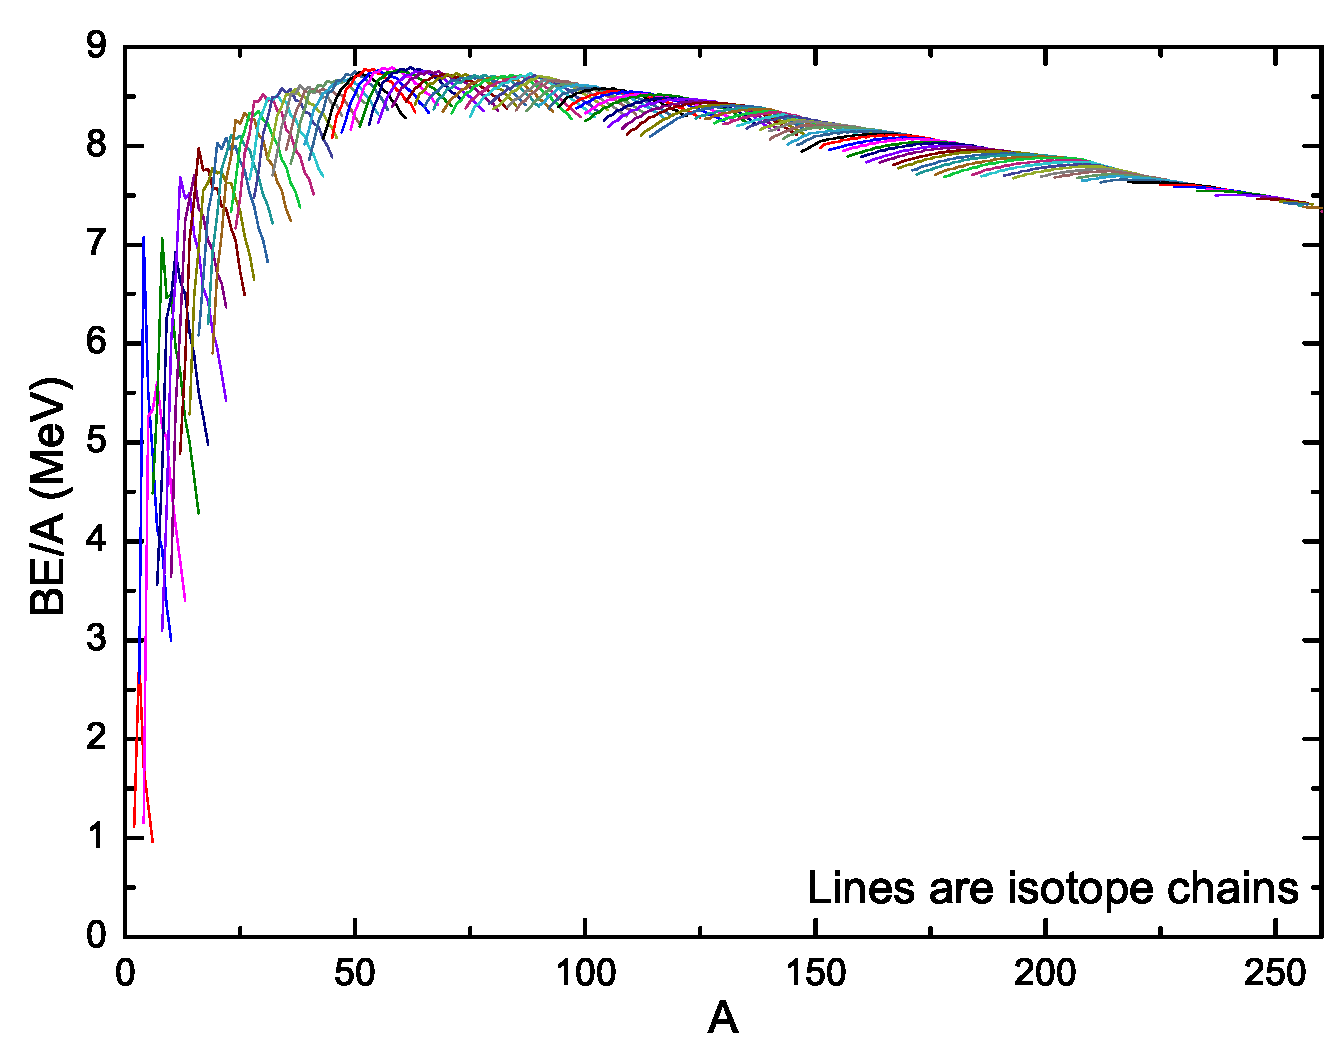
\includegraphics[width=\textwidth]{./img/c2/binding_plot.eps}}
	\caption{Binding energies per nucleon plotted versus mass number. Values calculated from Ref. \cite{AME20031,AME20032}.\label{fig:chp2-binding}}
\end{figure}

Examination of the two proton and two neutron separation energies (Fig. \ref{fig:chp2-masses}) shows several distinct discontinuities at specific numbers of protons or neutrons. Further examination of the energies of the first $2^+$ (Fig. \ref{fig:chp2-two-plus-energies}) states shows peaks at the same numbers. These ``magic numbers'' occur at numbers of protons and neutrons where there is a dramatic drop off in the nucleon separation energy with the addition of another nucleon. Further evidence for magic numbers of protons and neutrons can be found in the increase first excited state energies located at these magic numbers, substantially decreased neutron absorption cross-sections at neutron magic numbers, and in the enhanced abundance of nuclides where N and Z are magic numbers. The magic numbers are $2$, $8$, $20$, $28$, $50$, $82$, and $126$, with $40$ and $64$ also weakly magic over certain ranges of N and Z.

\begin{figure}[h!]
\centerline{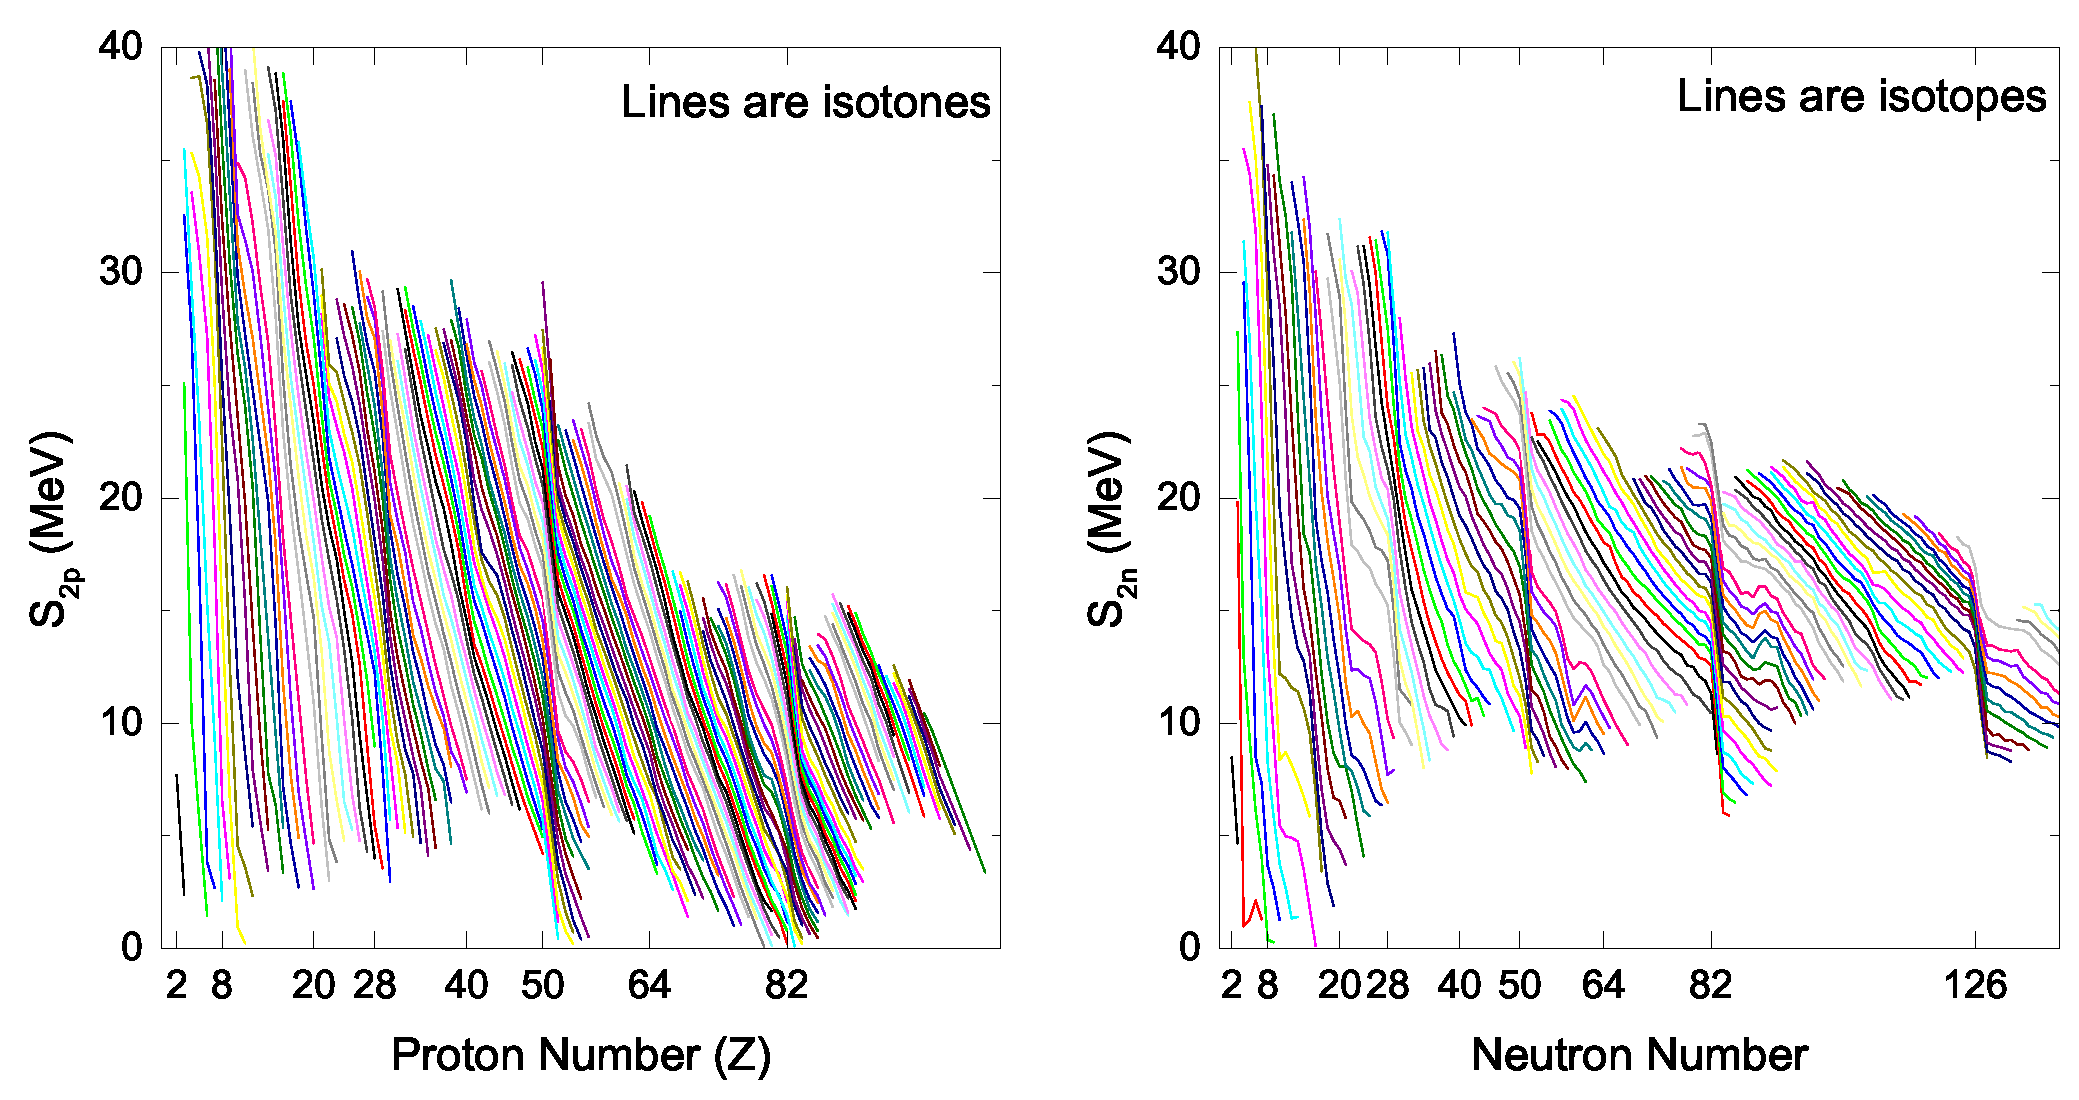
\includegraphics[width=\textwidth]{./img/c2/2nuc_sep_en.eps}}
	\caption{Left: Two proton separation energies plotted versus proton number. Each line is a set of isotones. Right: Two neutron separation energies plotted versus neutron number. Each line is a set of isotopes. Values calculated from Ref. \cite{AME20031,AME20032}.\label{fig:chp2-masses}}
\end{figure}

\begin{figure}[h!]
\centerline{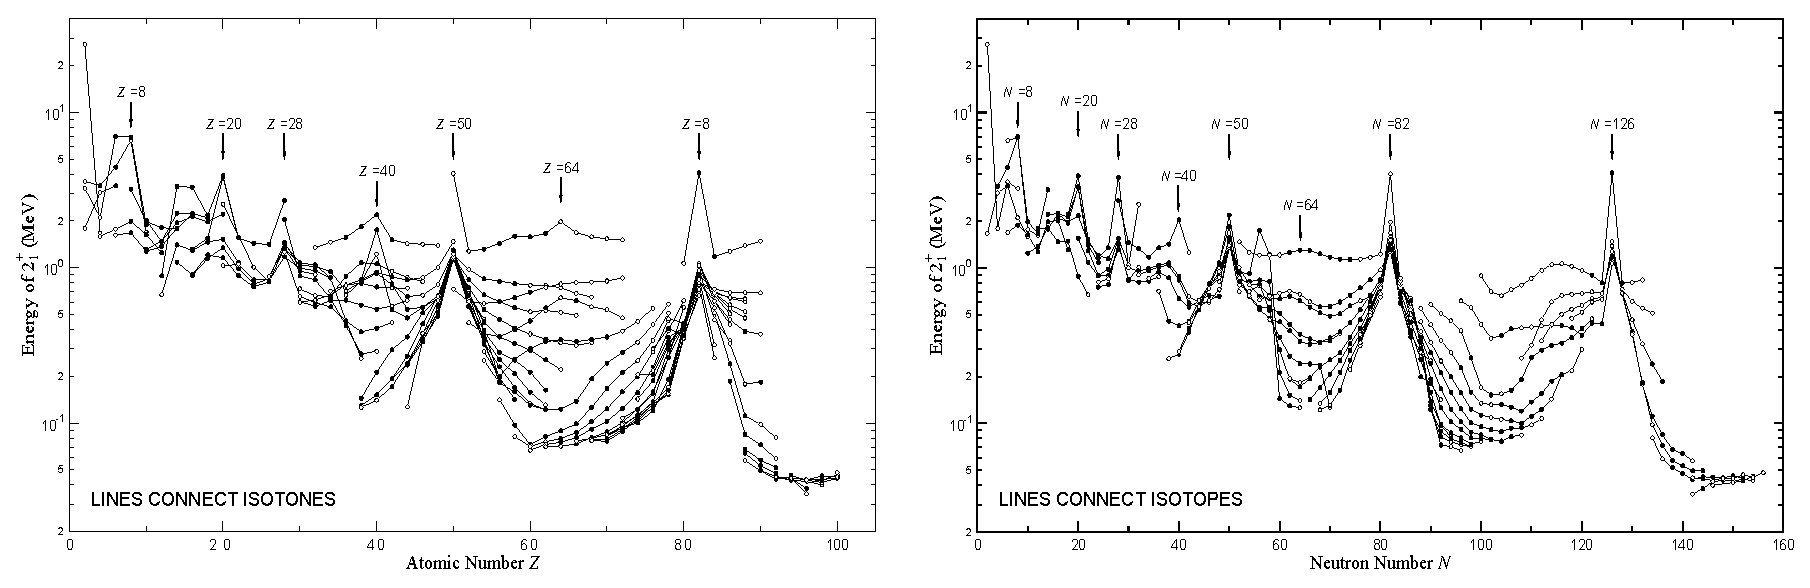
\includegraphics[width=\textwidth]{./img/c2/2_plus_en.eps}}
	\caption{Left: First excited $2^+$ energies of nuclei with even Z and N, plotted versus proton number. Each line is a set of isotones. Right: First excited $2^+$ energies of nuclei with even Z and N, plotted versus neutron number. Each line is a set of isotopes. Figures adapted from Ref. \cite{RamanTwoPlus}.\label{fig:chp2-two-plus-energies}}
\end{figure}

Analogy to atomic theory shows these magic numbers are major shell closures. This leads to the conclusion that the nucleus has shell structure, leading to the shell model of the nucleus. These numbers can be derived from the calculation of a single particle in a mean field potential. Far from stability, quenching of the known shell gaps and the opening of new shell gaps has been observed \cite{changingShells}.

The nucleus also exhibits collective excitations such as rotation and vibration which are described later in the chapter. The crucial differences between an atomic system and the nuclear system are as follows: First, the atom has a nucleus whose Coulomb field guides the electron cloud, preventing collective motions. Second, the nucleus has two types of particles, protons and neutrons, occupying its shells.. With this, certain shell occupations can lead to the ``single particle behavior'' exhibited around closed shells, while different occupations can yield collective phenomena.

\section{The Shell Model}
\label{sec:models-shell-model}
The nuclear shell model, in its simplest form, seeks to explain the shell structure observed in nuclei by describing them and independent particles in a mean field potential produced by the other nucleons. While the short range nature of the nuclear force might lead to the use of a square well potential or similar as the mean field, the Simple Harmonic Oscillator (SHO) potential is a reasonable first order approximation (seen in Figure \ref{fig:chp2-SHOPot}), which happens to be much simpler to solve. Placing a single particle in the SHO potential gives the first few magic numbers observed; however, to reproduce all the magic numbers it is necessary to add an $\vec{l}^2$ potential and a strong spin-orbit ($\vec{l}\cdot\vec{s}$) potential. The Hamiltonian for such a potential is as follows:
\begin{equation}
\label{eqn:chp2-sm-sho-hamil}
\mathbf{\mathit{H}} = \frac{-\hbar^2}{2m}\nabla^2 + \frac{1}{2}m(\omega r)^2 + B \uvec{l}^2 + A \uvec{l}\cdot{}\uvec{s}
\end{equation}
The progression of shell gaps from $SHO$ to $SHO + \vec{l}^2$ to $SHO + \uvec{l}^2 + \uvec{l}\cdot\uvec{s}$ is shown in Figure \ref{fig:chp2-shell-model}.

\begin{figure}
\centerline{\includegraphics[height=0.25\textheight]{./img/c2/sho_approx.png}}
	\caption{Schematic of a square well, SHO potential, and a realistic Woods-Saxon potential. Figure adapted from Ref. \cite{casten}.\label{fig:chp2-SHOPot}}
\end{figure}

\begin{figure}
\centerline{\includegraphics[height=0.45\textheight]{./img/c2/shell_model.png}}
	\caption{Spectrum of a single nucleon in an SHO potential, SHO + centrifugal potential, and, SHO + centrifugal + spin-orbit. Figure adapted from Ref. \cite{casten}.\label{fig:chp2-shell-model}}
\end{figure}

%TODO: Talk about quantum numbers and the like

In more realistic shell model calculations a Woods-Saxon potential is adopted. Here the Hamiltonian becomes:
\begin{equation}
\label{eqn:chp2-sm-ws-hamil}
\mathbf{\mathit{H}} = \frac{-\hbar^2}{2m}\nabla^2 + \frac{V}{1+e^{(r-R)/a}} - \alpha(r)\uvec{l}\cdot\uvec{s}
\end{equation}
where $R=r_0A^{1/3}$, $r_0\sim1.2$fm, $a\sim0.5$fm, and $V\sim50$MeV. In addition to the central term, a spin orbit term is necessary to reproduce the observed shell gaps. The central flatness of the Woods-Saxon potential reflects the saturation of the nuclear force better than an SHO potential. This increased realism comes at the cost of increased difficulty in calculations--with this Hamiltonian the Sch\"odinger equation is no longer analytically solvable and must instead be solved with numerical methods.
%and the loss of quantum numbers; in this model the only good quantum numbers are $J=\mathit{l}+\mathit{s}$ and $\pi = (-1)^\mathit{l}$.

Up to now in this chapter, the nucleons were considered as independent particles within a mean field which was the average potential produced by the other particles. This description, while powerful, is not accurate, especially for nuclei away from the closed shells. The missing piece is the interactions between nuclei that are not accounted for in the mean field, often called ``residual interactions.'' Residual interactions must be accounted for to produce an accurate description of the nucleus.

\section{The Deformed Shell Model}
\label{sec:models-shell-model-def-sm}
\subsection{Parameterization of Deformation}
\label{ssec:models-shell-model-def-param}
In the standard shell model the potentials are spherically symmetric, depending only on the radius. While this is a successful approach near the shell gaps where nuclei are spherical, or nearly spherical, it breaks down in the deformed regions farther from shell closures. In such nuclei, the long-range correlations experienced by the valence nucleons can lead to deformation as the valence nucleons are arranged into deformed shells with lower energy levels. When the nuclear shape is deformed the surface of the nucleus is described with a parametric function defining the radius as follows:
\begin{equation}
\label{eqn:surface-full-expansion}
R(\theta, \phi) = R_{o}\left \lgroup 1 + \sum_{\lambda = 2}^{\infty}\sum_{\mu = -\lambda}^{\lambda}\alpha_{\lambda \mu} Y_{\lambda \mu}(\theta, \phi)\right \rgroup
\end{equation} 
Here $R_0$ is the radius of a sphere with the same volume as the deformed nucleus, $Y_{\lambda \mu}(\theta, \phi)$ are the spherical harmonic functions, and $\alpha_{\lambda \mu}$ are the coefficients of the expansion. The expansion starts at $\lambda = 2$ because the $\lambda = 1$ corresponds to the translation of the center of mass, a term easily eliminated by requiring the nuclear center of mass to coincide with the coordinate's origin. The first of the non-trivial terms, $\lambda = 2$, corresponds to the components of quadrupole deformation, $\lambda = 3$ gives octupole deformation, $\lambda = 4$ gives hexadecapole deformation, and so on. As $\lambda = 2$ is the most important component in this work, only quadrupole deformation terms will be considered henceforth.

The quadrupole shapes cover oblate spheres (two semi-major axes, like a doorknob), prolate spheres (two semi-minor axes, like an American football), and triaxial shapes (all three axes are different lengths, like a potato). Because the rotation of the nucleus is not fixed, \emph{i.e.} the nucleus can be rotated such that its principal axes coincide with the axes of the coordinate system, the five quadrupole shape parameters are reduced to two independent parameters $a_{2 0}$ and $a_{2 2}$, with the conditions: $a_{2 -2}=a_{2 2}$ and $a_{2 1}=a_{2 -1}=0$. Further, it is common to parameterize the remaining expansion coefficients using the Hill-Wheeler variables, $\beta$ and $\gamma$, as follows \cite{wongBook}:
\begin{align}
\label{eqn:chp2-hill-wheeler}
a_{2 0} = \beta \cos(\gamma)  & &  a_{2 2} = a_{2 -2} = \frac{1}{\sqrt{2}}\beta \sin(\gamma)
\end{align}
Expanding the spherical harmonics as:
\begin{align}
\label{eqn:spherical-harmonics}
Y_{2 0}(\theta, \phi) &= \frac{1}{4} \sqrt{\frac{5}{\pi }} \left(-1+3 \cos(\theta )^2\right)\\
Y_{2 2}(\theta, \phi) &= \frac{1}{4} e^{2 i \phi } \sqrt{\frac{15}{2 \pi }} \sin(\theta)^2\\
Y_{2 -2}(\theta, \phi) &= \frac{1}{4} e^{-2 i \phi } \sqrt{\frac{15}{2 \pi }} \sin(\theta)^2
\end{align} 
and inserting all this into Equation \ref{eqn:surface-full-expansion} yields:
\begin{equation}
\label{eqn:quadrupole-surface}
R(\theta, \phi) = R_{o}\left(1+\sqrt{\frac{5}{16 \pi }}\beta  \left(\cos(\gamma ) \left(3 \cos(\theta )^2-1\right)+\sqrt{3} \sin(\gamma ) \sin(\theta )^2\cos(2 \phi )\right)\right)
\end{equation} 
The Hiller-Wheeler variables have some redundancy: for $\beta>0$ the nucleus is prolate for $\gamma=0^{\circ},120^{\circ},240^{\circ}$ and oblate for $\gamma=180^{\circ},300^{\circ},60^{\circ}$. However, for $\gamma=0^{\circ}$ and $\gamma=180^{\circ}$ the symmetry axis is the $\uvec{z}$-axis of the intrinsic frame, for $\gamma=120^{\circ}$ and $\gamma=300^{\circ}$ the symmetry axis is the $\uvec{x}$-axis, and for $\gamma=240^{\circ}$, and $\gamma=60^{\circ}$ the symmetry axis is the $\uvec{y}$-axis. The Lund convention makes use of this redundancy by selecting a rotational axis according to the following rules \cite{wongBook}:
\begin{enumerate}
\item $\beta\geq0$
\item For rotation about the smallest axis $0^{\circ}\leq\gamma\leq60^{\circ}$
\item For rotation about the longest axis $-120^{\circ}\leq\gamma\leq-60^{\circ}$
\item For rotation about the intermediate axis $-60^{\circ}\leq\gamma\leq0^{\circ}$
\end{enumerate}
A graphical schematic of the Lund convention is in Figure \ref{fig:chp2-lund}
\begin{figure}[t!]
\label{fig:chp2-lund}
\centerline{\includegraphics[height=0.25\textheight]{./img/c2/lundconv.png}}
	\caption{Schematic of the Lund convention. Figure adapted from Ref. \cite{danielDissertation}.}
\end{figure}
\subsection{The Nilsson Model}
In 1955, to treat deformed nuclei, S.G. Nilsson introduced a modified version of the shell model in Ref. \cite{nilsson}. This modified shell model, known as the Nilsson model, allows deformation to be taken into account using an anisotropic harmonic oscillator potential as follows:
\begin{equation}
\label{eqn:chp2-nilsson-hamil}
H_{nil}=-\frac{\hbar^{2}}{2m}\nabla^{2} + \frac{m}{2}\left(\omega_{x}^{2}x^{2} + \omega_{y}^{2}y^{2} + \omega_{z}^{2}z^{2}\right) + 2\kappa \hbar \omega_{o}\left[\vec{l}\cdot \vec{s} - \mu \left(l^{2} - \left \langle l^{2} \right \rangle_{N} \right) \right]
\end{equation} 
Here $\omega_{x,y,z}$ are the oscillator frequencies in each of the three dimensions, $\kappa$ controls the strength of the spin orbit part of the potential, and $\mu$ controls the strength of the correction term. The correction term, $l^2 - \left \langle l^{2} \right \rangle_{N}$, originally had the form of $\mu l^2$ \cite{nilsson}. It served the purpose of suppressing the energy of the higher lying shells; however, it was noted in Ref. \cite{nilssonCorrection} that this shift was too large for large N quantum numbers. Thus the correction term was modified to its current form to compensate. The three oscillator frequencies are chosen to be inversely proportional to the axis lengths of the ellipsoid $a_x$, $a_y$, and $a_z$ as follows:
\begin{align}
\label{eqn:chp2-nilsson-oscilator-freq}
\omega_i = \omega_0\frac{R_0}{a_i} &  & i=x,y,z
\end{align}
Here $\omega_0$ is the oscillator frequency for the spherical case, defined as $\hbar\omega_0 = (\omega_x \omega_y \omega_z )^{1/3}$. In the case of axial symmetry the oscillator frequencies are defined in terms of the deformation parameter $\epsilon_2$ as follows.
\begin{align}
\label{eqn:chp2-nilsson-oscilator-freq-components}
\omega_{x}=\omega_{y}=\omega_{\bot}&=\omega(\epsilon_2)\left(1+\frac{1}{3}\epsilon_2 \right)\\
\omega_{z}=\omega_{\parallel}&=\omega(\epsilon_2)\left(1-\frac{1}{3}\epsilon_2 \right)\\
\omega(\epsilon_2) &= \omega_0\left(1-\frac{1}{3}\epsilon_2^2-\frac{2}{27}\epsilon_2^3\right)^{-1/6}
\end{align}
Here the deformation $\beta$ is defined with respect to $\epsilon_2$ using the following series:
\begin{align}
\label{eqn:chp2-nilsson-beta-from-epsilon}
\beta = \sqrt{\frac{16 \pi}{5}}\left( \frac{1}{3}\epsilon_2 + \frac{1}{9}\epsilon_2^2 + \frac{1}{27}\epsilon_2^3 +  \frac{1}{81}\epsilon_2^4...\right)
\end{align}

With these definitions and the Nilsson Hamiltonian, the energy eigenstates ($\epsilon_{\Omega[Nn_z\Lambda]}$), sometimes called Nilsson orbitals, can be extracted from solving the Sch\"odinger equation.
\begin{equation}
\label{eqn:chp2-schodinger-eqn-nilsson}
H_{nil}\psi_{i}=\epsilon_{i}\psi_{i}
\end{equation}
Here $i$ represents the complete set of asymptotic quantum numbers used to specify Nilsson orbitals:
\begin{equation}
\label{eqn:chp2-nilsson-numbers}
\Omega^{\pi}[Nn_z\Lambda]
\end{equation}
$\Omega$ is projection of the particle's total angular momentum onto the symmetry axis, $\pi$ is the parity defined as $\pi=(-1)^{l}=(-1)^{N}$, $N$ is the oscillator quantum number, $n_z$ is the number of oscillator quanta (number of nodes in the wave function), and $\Lambda$ is the projection of the particle's orbital angular momentum onto the symmetry axis. Some of these quantum numbers are shown schematically in Fig. \ref{fig:chp2-nillson-qn}. 

\begin{figure}[hb!]
\centerline{\includegraphics[height=0.22\textheight]{./img/c2/nilsondescr.png}}
	\caption{Schematic of an axially symmetric nucleus and the various quantum numbers that are used in the description of the system. Here R is the angular momentum of collective rotation, J is the total nuclear angular momentum, j is the total angular momentum of the particle, l is the orbital angular momentum of the particle, s is the spin of the particle, M is the projection of J onto the non-symmetry axis, K is the projection of J onto the symmetry axis, $\Omega$ is the projection of j onto the symmetry axis, $\Lambda$ is the projection of l onto the symmetry axis, and $\Sigma$ is the projection of s onto the symmetry axis. Figure adapted from Ref. \cite{danielDissertation}.\label{fig:chp2-nillson-qn}}
\end{figure}

The deformation dependence of Nilsson orbitals is usually summarized in a Nilsson diagram. In these diagrams energy levels for various sets of asymptotic quantum numbers are plotted versus the deformation parameter $\epsilon$. A Nilsson diagram for protons in the $40\leq{}Z\leq82$ region is shown in Fig. \ref{fig:chp2-nillson-protons}. A diagram for neutrons in the $40\leq{}Z\leq82$ region is shown in Fig. \ref{fig:chp2-nillson-neutrons}. Together these diagrams cover the $A\sim 130$ region where \pr{} lies.

\begin{figure}[h!]
\centerline{\includegraphics[height=0.8\textheight,clip=true,trim=10 100 10 100]{./img/c2/nilsson_proton_diagram.pdf}}
	\caption{Nilsson diagram for protons in the $50\leq Z \leq 82$ region with $\epsilon_4=\epsilon_2/6$. Solid lines represent positive parity orbitals and dashed lines represent negative parity orbitals. Labels follow the $\Omega$[N $n_z$ $\Lambda$] convention. Figure adapted from Ref. \cite{nilssonDiagrams}.\label{fig:chp2-nillson-protons}}
\end{figure}

\begin{figure}[h!]
\centerline{\includegraphics[height=0.8\textheight,clip=true,trim=10 100 10 100]{./img/c2/nilsson_neutron_diagram.pdf}}
	\caption{Nilsson diagram for neutrons in the $50\leq N \leq 82$ region with $\epsilon_4=\epsilon_2/6$. Solid lines represent positive parity orbitals and dashed lines represent negative parity orbitals. Labels follow the $\Omega$[N $n_z$ $\Lambda$] convention. Figure adapted from Ref. \cite{nilssonDiagrams}.\label{fig:chp2-nillson-neutrons}}
\end{figure}

\section{Collective Rotation}
\label{sec:models-rigid-rotor}
A model of collective nuclear motion was developed by Bohr and Mottleson \cite{bohrMottelsonArticle,bohrMottelson2} due to several observations that could not be explained with single particle motion. Among these are: \emph{1.} Fission, many of the features are successfully explained with the liquid drop model \cite{meitnerFissionProducts,fissionMechanism}. \emph{2.} Deformation of the nuclear surface by particle structure \cite{deformationPrediction} giving rise to quadrupole moments which exceed single particle estimates in many nuclei \cite{casimirQuadMoments,nuclearQuadMomentsAndShellStruc}. \emph{3.} The occurrence of electric quadrupole gamma ray transitions with lifetimes much shorter than single particle estimates \cite{nuclearIsomerClassification} which is a characteristic feature of the excitation spectra of strong deformed nuclei and most importantly: rotational bands \cite{QuadIsomerInterp}.
\subsection{Rigid Triaxial Rotor Model (TRM)}
\label{ssec:models-triaxial-rotor}
One of the simplest forms of excitation a nucleus can experience is rotation. However, in quantum mechanics rotation is can only occur about axes that are not symmetry axes (where the symmetry axis is denoted the $\uvec{z}$-axis). This is because the wave function that describes this system is an eigenfunction of $\uvec{J}_z$, and thus, is symmetrical about the $\uvec{z}$-axis. Due to this symmetry any rotation of this wave function about the symmetry axis generates only phase shift and has a wave function identical to that of the ground state. A system cannot collectively rotate about symmetry axes. Since spherical nuclei are symmetric about all axes, they cannot exhibit collective rotation.

In rotating nuclei there are two primary components of the angular momentum. The first is the rotational angular momentum, $\vec{R}$, generated by the collective motion of many nucleons about some axis. The second component is found when there are unpaired valence nucleons. In these cases their angular momentum, $\vec{j}$, must be accounted for as well. This presents a situation like that in Figure \ref{fig:chp2-nillson-qn} which schematically illustrates the total angular momentum of the nucleus, $\vec{J}$, as the sum of $\vec{R}$ and $\vec{j}$.

While it is often the case that the shape (and thus the moments of inertia (MOI)) of a nucleus changes somewhat as spin increases, accounting for this can be difficult. By approximating the system as a rigid rotor with unchanging MOI the problem can be simplified while maintaining descriptive power. Here each axis has a fixed MOI and the rotational component of the Hamiltonian depends only on the MOIs and the components of the spin along each axis. In the case of a triaxial nucleus with no unpaired valence particles, (thus $\vec{J}=\vec{R}$) the Hamiltonian can be written as follows \cite{triaxRotorSol,wobblingGeometry}:
\begin{align}
\label{eqn:chp2-triaxial-rotor-hamiltonian}
H &= H_{rot} + H_{intr} \\
H_{rot}&=A_3\uvec{J}_3^2 + A_1\uvec{J}_1^2 + A_2\uvec{J}_2^2
\end{align}
Here $H_{intr}$ is the intrinsic component of the Hamiltonian accounting for the internal state of the nucleus, $A_i = \frac{\hbar^2}{2 \mathcal{J}_i}$ where $\mathcal{J}_i$ is the MOI of rotation about the $i^{th}$ axis, and $\uvec{J}_i$ is the operator for the component of the angular momentum along the $i^{th}$ axis. Rewriting the rotational Hamiltonian to a form that uses the operators $\uvec{J}^2$, $\uvec{J}^2_3$, and $\uvec{J}^2_{\pm}$ yields:
\begin{align}
\label{eqn:chp2-triaxial-rotor-hamiltonian-rewrite}
H_{rot}=& H_{r}^{Diag} + H_{r}^{OffDiag}\\
H_{r}^{Diag}=&\left[\frac{1}{2}\left(A_1+A_2\right)\uvec{J}^2 + \left(A_3-\frac{1}{2}\left(A_1+A_2\right)\right)\uvec{J}^2_3\right]\nonumber\\
H_{r}^{OffDiag}=&\frac{1}{4}\left(A_1-A_2\right)\left(\uvec{J}^2_++\uvec{J}^2_-\right) \nonumber
\end{align}
Here $H_{r}^{Diag}$ is the diagonal component of the Hamiltonian, $H_{r}^{OffDiag}$ is the off diagonal component, $\uvec{J}^2$ is the total angular momentum operator, and $\uvec{J}^2_{\pm}$ are the angular momentum raising and lowering operators $\uvec{J}_{\pm} = \uvec{J}_1\pm\mathit{i}\uvec{J}_2$. Taking the basis states of the wave function to be \cite{triaxRotorSol}:
\begin{equation}
\label{eqn:chp2-triaxial-rotor-basis}
\Ket{IMK}= \sqrt{\frac{2I+1}{16\pi^{2}(1+\delta_{K0})}} \left[\mathcal{D}^{J}_{MK} + (-1)^J \mathcal{D}^{J}_{-KM}\right]
\end{equation}
Where $\delta_{K0}$ is the Kronecker delta function and $\mathcal{D}^{J}_{MK}$ are the Wigner D-functions which are functions of the three Euler angles that determine the orientation of the nucleus's principal axes in space. With these basis states the Hamiltonian matrix can be calculated and the energy eigenvalues and eigenstates for a given spin I is a matter of diagonalizing the matrix. The reduced transition probabilities for $E2$ transitions of the triaxial rotor model are given by \cite{wobblingGeometry}:

%the diagonal portion of the Hamiltonian matrix is:
%\begin{equation}
%\label{eqn:chp2-triaxial-diagonal-hamil}
%\Bra{IMK}H_{rot}\Ket{IMK}=\frac{1}{2}\left(A_1+A_2\right)\left(J(J+1)-K^2\right) + A_3K^2
%\end{equation}
%Similarly the off diagonal components are:
%\begin{equation}
%\label{eqn:chp2-triaxial-offdiagonal-hamil}
%\Bra{IMK}H_{rot}\Ket{IMK\pm{}2}=\frac{1}{4}\left(A_1-A_2\right)\sqrt{(I\mp{}K)(I\pm{}K+1)(I\mp{}K-1)(I\pm{}K+2)}
%\end{equation}
%With these, finding the energy eigenvalues and eigenstates for a given spin I is a matter of diagonalizing the matrix. The reduced transition probabilities for $E2$ transitions of the triaxial rotor model are given by \cite{wobblingGeometry}:
\begin{align}
\label{eqn:chp2-triaxial-rotor-reduced-transitions}
B\left(E2,I\rightarrow{}I'\right) &=\sum\limits_{\mu{},K,K'}^{}|\Bra{I'M'K'}\mathcal{M}^E_{2\mu}\Ket{IMK}|^2\\
\mathcal{M}^E_{2\mu} &= \sqrt{\frac{5}{16\pi}}\left[\mathcal{D}^{2*}_{\mu{}0}\uvec{Q}'_{20}+\left(\mathcal{D}^{2*}_{\mu{}2}+\mathcal{D}^{2*}_{\mu{}-2}\right)\uvec{Q}'_{22}\right] \nonumber\\
Q'_{20} &= Q \cos(\gamma) ~~~~~~~ Q'_{22} = \frac{1}{\sqrt{2}}Q \sin(\gamma) \nonumber
\end{align}

\subsection{Quasiparticle + Triaxial Rotor (QTR)}
\label{sec:models-qtr}
The QTR model is an extension of the particle + rotor model which was put forth in its earliest form in 1952 by Aage Bohr in Ref. \cite{bohrParticlePlusRotor}. This model allows the calculation of the effect of coupling the odd quasiparticle to the triaxial even-even core. The lab frame Hamiltonian of this model is given in Ref. \cite{frauendorfTransverseWobbling} to be:
\begin{align}
\label{eqn:chp2-qtr-hamil}
H&=H_{sqp}+H_{rot}-H_{int}\\
%H_{rot}&=A_3(\uvec{J}_3-\uvec{j}_3)^2+A_1(\uvec{J}_1-\uvec{j}_1)^2+A_2(\uvec{J}_2-\uvec{j}_2)^2\\
H_{rot}&=A_3\uvec{R}_3^2+A_1\uvec{R}_1^2+A_2\uvec{R}_2^2\\
H_{int}&=\kappa \sum\limits_{\mu}^{}q^*_{\mu}Q_{\mu} = \kappa{} f r^2 \left(\epsilon \cos(\gamma) \bar{Y}^2_0 + \frac{\epsilon \cos(\gamma)}{\sqrt{2}}\left(\bar{Y}^2_2 + \bar{Y}^2_{-2}\right)\right)
\end{align}
Here $H_{sqp}$ is the single quasiparticle Hamiltonian accounting for the presence of the central potential and the pairing interaction, $H_{rot}$ is the rotor model Hamiltonian, $H_{int}$ is the interaction of the quasiparticle to the triaxial core, $\uvec{J}_k$ is the total angular momentum of the system along the $k^{th}$ axis, $\uvec{j}_k$ is the angular momentum of the quasiparticle along the $k^{th}$ axis, $\bar{Y}^l_m$ is the result of applying the spherical harmonic operator $Y^l_m$ to the basis state, $f$ is the scaling factor obtained from the following:
\begin{align}
\label{eqn:chp2-qtr-int-hamil-scaling}
\kappa f = \frac{2}{3}\sqrt{\frac{4\pi}{5}}\hbar\omega_{\circ}\\
\end{align}
and $\kappa$ is the coupling strength, which is related to the deformation of the system by:
\begin{align}
\label{eqn:chp2-qtr-int-hamil-coupling}
\kappa \Bra{0}|Q|\Ket{2} & = \hbar\omega_{\circ} \epsilon \cos(\gamma)
\end{align}
Here $\Bra{0}|Q|\Ket{2}$ is the reduced matrix element of the core quadrupole operator between the  $0^+$ ground state and the first $2^+$ state. This is related to the reduced quadrupole transition probability as follows:
\begin{equation}
\label{eqn:chp2-red-mat-el-to-red-trans-prob}
B(E2,J_I\rightarrow{}J_F)=\frac{|\Bra{J_F}|Q|\Ket{J_I}|^2}{2J_I+1}
\end{equation}

Qualitatively, the $H_{int}$ works as follows. A high j quasiparticle with predominantly particle nature will align its $\vec{j}$ to the short axis of the core. This orientation results in the maximum overlap of the torus like density distribution of the quasiparticle and the triaxial core which minimizes the energy of the attractive interaction between the two. For a high j quasiparticle with hole nature, the $\vec{j}$ aligns to the long axis which minimizes the overlap of the torus with the triaxial core and minimizes the energy of the repulsive interaction between the two. Finally a quasiparticle from the middle of the shell, possessing particle and hole nature in roughly equal measure, would align the medium axis of the triaxial core.

The reduced transition probabilities of this system can be extracted similarly to those of the triaxial rotor model (equation \ref{eqn:chp2-triaxial-rotor-reduced-transitions}); however the operator $\mathcal{M}^E_{2\mu}$ will change to account for the quadrupole moment of both the core ($Q$) and the quasiparticle ($q$).

\subsection{Pairing}
\label{ssec:models-pairing}
The pairing interaction is the force that couples two identical nucleons in time reversed orbits (opposite spin projections). Evidence for this force can be seen in a variety of experimental results, among them: 1) The staggering seen in the single neutron (or proton) separation energies between even and odd neutron (or proton) number (see Fig. \ref{fig:chp2-s1n-staggering}); 2) The ground state of \emph{every} even-even nucleus has $J^{\pi}=0^+$; and 3) The ground states of the odd-A nuclei always have $J^{\pi}$ determined by the orbital of the last unpaired nucleon.

\begin{figure}[t!]
\centerline{\includegraphics[height=0.3\textheight]{./img/c2/S1n_MassChains.eps}}
	\caption{One neutron separation energies vs neutron number for the five isotopes from $Z=51$ to $Z=55$. The staggering between even and odd masses gives strong evidence for the pairing interaction. Additionally the $N=82$ shell gap can be seen. Figure adapted from Ref. \cite{nilssonDiagrams}.\label{fig:chp2-s1n-staggering}}
\end{figure}

%In 1950, M. Goeppert suggested the first theoretical tool to calculate this interaction \cite{pairingFirstTheory} describing the pairing force as a delta function multiplied by some interaction strength.
%\begin{equation}
%\label{eqn:chp2-pairing-first-function}
%V_{pair}=-G\delta(\phi_1-\phi_2)\delta(\cos(\theta_1)-\cos(\theta_2))\frac{\delta(r_1-r_2)}{r^2}
%\end{equation}
In 1950, M. Goeppert suggested describing the pairing force as a delta function multiplied by some interaction strength \cite{pairingFirstTheory}. Calculations were performed using this interaction to explore its effects \cite{pairingCorrEffectOnProperties} and then later analogies between nuclear pairing and BCS superconductivity theory \cite{bcsTheory} were discovered and examined \cite{pairingAnalogyToBCS,pairingSuperfluidity}. The pairing interaction strength $G$ has been determined to have different values for the protons and neutron. For protons the pairing strength is approximately $G_p=\frac{17}{A} MeV$ and for neutrons the pairing strength is approximately $G_n=\frac{23}{A} MeV$. The Hamiltonian to describe this interaction is usually written as:
\begin{equation}
\label{eqn:chp2-pairing-hamil}
H_{pair} = -GP^+P-\lambda{}\uvec{N}
\end{equation}
%The expectation value for this interaction is:
%\begin{equation}
%\label{eqn:chp2-pairing-expectation}
%\Braket{j_1j_2J|V_{pair}|j3j4J'}=-G\sqrt{\left(j_1+\sfrac{1}{2}\right)\left(j_3+\sfrac{1}{2}\right)}\delta_{j_1j_2}\delta_{j_3j_4}\delta_{J0}\delta_{J'0}
%\end{equation}
%In the second quantization formalism, the pairing Hamiltonian is usually written in the form:
Here, $\lambda$ is the chemical potential and $\uvec{N}$ is the particle number operator, together these give particle number conservation. Finally, $P^+$ is the monopole pair field, expressed by:
\begin{equation}
\label{eqn:chp2-monopole-pair-op}
P^+=\sum\limits_{k>0}^{}c^+_kc^+_{\bar{k}}
\end{equation}
Here $\bar{k}$ represents the time reversed state of $k$, \emph{i.e.} spin-up $\rightarrow$ spin-down.

If the spacing between levels near the Fermi surface is small relative to $G$ then the pairing interaction scatters pairs of nucleons with $J^{\pi}=0^+$ from occupied levels to empty levels above the Fermi level. This results in the ``smeared'' nucleon distribution shown in the dashed line of Fig. \ref{fig:chp2-pairing-fermi-surface}. If the level spacing is large near the Fermi surface then the pairing interaction cannot scatter pairs into unoccupied levels and the Fermi surface has a sharp cutoff as seen in the solid line of Fig. \ref{fig:chp2-pairing-fermi-surface}.
\begin{figure}[t!]
\centerline{\includegraphics[height=0.3\textheight]{./img/c2/pairinginteraction.png}}
	\caption{Schematic of the occupancy of single particle states with and without pairing. Figure adapted from Ref. \cite{xfwangDissertation}.\label{fig:chp2-pairing-fermi-surface}}
\end{figure}

The energy range that this ``smearing'' of level occupancies covers is equal to the gap parameter ($\Delta$) which can be defined as follows:
\begin{equation}
\label{eqn:chp2-pairing-gap-param}
\Delta = G\sum\limits_{ij}^{}U_iV_j
\end{equation}
Where $U$ is the emptiness factor (the probability that a state will be occupied by a hole) and $V$ is the fullness factor (the probability that a state will be occupied by a particle). $U$ and $V$ are defined as follows
\begin{align}
\label{eqn:chp2-pairing-gap-param-defs}
V_i &= \sqrt{\frac{1}{2}\left(1+\frac{\epsilon_i-\lambda}{\sqrt{(\epsilon_1-\lambda)^2+\Delta^2}}\right)}\\
U_i &= \sqrt{\frac{1}{2}\left(1-\frac{\epsilon_i-\lambda}{\sqrt{(\epsilon_1-\lambda)^2+\Delta^2}}\right)}
\end{align}
Here $\epsilon_i$ represents the single particle energies, and $\lambda$ is the chemical potential for a given number of particles. The probabilities are normalized such that $U_i^2+V_i^2=1$. Far below the Fermi surface the probability that an orbit will be occupied is $V_i=1$, while the probability that the orbit is unoccupied $U_i=0$. This situation reverses itself far above the Fermi surface. Close to the Fermi surface both probabilities will have a finite value. In BCS theory \cite{bcsTheory} the quasiparticle energy is expressed as:
\begin{equation}
\label{eqn:chp2-pairing-qp-en}
E_{qp}(n,p)=\sqrt{(\epsilon_i-\lambda)^2+\Delta^2}
\end{equation}

As the nucleus rotates the induced Coriolis force competes with the pairing interaction. The competition attempts to break the pairs and align the individual angular momenta of the nucleons with the rotation axis. In general rotational motion weakens the pairing strength in the nucleus. While some pairs break and align at specific rotational frequencies, all pairs experience the effects. This phenomenon is called the Coriolis anti-pairing effect (CAP) \cite{bohrMottelsonRotationWeakensPairing}.

\subsection{Tilted Axis Cranking}
\label{sec:models-tac}
%The tilted axis cranking (TAC) model \cite{frauendorfTAC} is a generalization of the cranked shell model introduced by Inglis in 1954 \cite{crankedShellModel}. In this model, nucleons are individual particles independently moving in an average potential, which in turn rotates about some axis. As expected of a rotating frame, the Coriolis and centrifugal forces play an important role in the TAC model with consequences for shape and pairing correlations. The Hamiltonian for this model has two terms, the cranking component $-\omega\uvec{J}_x$ which represents the centrifugal and Coriolis forces from the rotating reference frame and a component in the rotating frame, $H_0$.
The tilted axis cranking (TAC) model \cite{frauendorfTAC} is a generalization of the cranked shell model introduced by R. Bengtsson and S. Frauendorf in \cite{crankedShellModelNonPeturbative}. In this model, nucleons are individual particles independently moving in an average potential, which in turn rotates about some axis. As expected of a rotating frame, the Coriolis and centrifugal forces play an important role in the TAC model with consequences for shape, pairing correlations, and quasiparticle orbitals. The Hamiltonian for this model has two terms, the cranking component $-\omega\uvec{J}_x$ which represents the centrifugal and Coriolis forces from the rotating reference frame and a component in the rotating frame, $H_0$.
\begin{equation}
\label{eqn:chp2-TAC-Hamiltonian}
H'=H_0-\omega\uvec{J}_x
\end{equation}
Ref. \cite{frauendorfTAC} starts with the pairing plus quadrupole Hamiltonian given by:
\begin{equation}
\label{eqn:chp2-TAC-invar-Hamiltonian}
H_0=H_{sph}-\frac{\chi}{2}\sum\limits_{\mu=-2}^{2}Q_{\mu}^+Q_{\mu} - GP^+P-\lambda\uvec{N}
\end{equation}
Here the spherical potential is simply parameterized as by the energy $\epsilon_k$ for a state labeled $k$ and then constructed in second quantization as:
\begin{equation}
\label{eqn:chp2-TAC-spherical}
H_{sph}=\sum\limits_{k}^{}\epsilon_kc^+_kc_k
\end{equation}
The short range pair correlations are accounted for using the monopole pair operator defined in Eqn. \ref{eqn:chp2-monopole-pair-op}. The quadrupole interaction operator accounts for the long range particle-hole interaction:
\begin{equation}
\label{eqn:chp2-TAC-quad}
Q_{\mu}=\sum\limits_{k,k'}^{}\sqrt{\frac{4\pi}{5}}\Bra{k}r^2Y_{2\mu}\Ket{k'}c^+_kc_{k'}
\end{equation}
Finally, the term $\lambda\uvec{N}$ accounts for the number of particles (N) using the chemical potential $\lambda$. As written the Hamiltonian of equation \ref{eqn:chp2-TAC-Hamiltonian} only accounts for one type of particles, protons or neutrons; thus all the expressions should be understood as sums across neutron and proton parts.

To determine the system wave functions,  $\ket{}$, the eigenstates of the Hartree-Fock-Bogoliubov (HFB) mean field Routhian are found. The HFB Routhian is:
\begin{equation}
\label{eqn:chp2-TAC-HFB-Routhian}
h'=h - \sum\limits_{\mu=-2}^{2}(q_{mu}Q^+_{\mu}+q^*_{mu}Q_{\mu}) - \Delta(P^++P) - \lambda{}N-\omega\uvec{J}_z
\end{equation}
Applying the self-consistency conditions: $q_{\mu}=\chi{}\braket{Q_{\mu}}$, $\Delta=G\braket{P}$, and conservation of particle number $N=\braket{\uvec{N}}$ gives the deformed potential $h$. Further information regarding operator definitions and procedures for self-consistent solutions can be found in References: \cite{frauendorfTAC,frauendorfTACMultiQPBands,nuclearManyBodyProblem}

As stated in Refs. \cite{timeDepVarMethodForRotation,frauendorfTACMultiQPBands}, self consistent solutions must have their angular frequency and angular momentum vectors parallel \emph{i.e.} $\vec{\omega}\parallel\vec{J}$. Additionally, self consistent solutions to the total Routhian ($E'=\braket{H'}$) satisfy the extremum conditions of:
\begin{equation}
\label{eqn:chp2-tac-extrema-cond}
\left. \frac{\partial{}E'}{\partial{}q_{\mu}} \right|_{\omega}=0 ~~~~~ \left. \frac{\partial{}E'}{\partial{}\Delta} \right|_{\omega}=0
\end{equation}
and have total energy and angular momentum:
\begin{align}
E(J)=E'(\omega)+\omega{}J(\omega) & & J(\omega) = \braket{\uvec{J}_z}
\end{align}

The orientation intrinsic frame is chosen such that the components of the quadrupole tenser satisfy $q'_{-1}=q'_1=0$ and $q'_{-2}=q'_2$. With this, the principal axes of the intrinsic frame coincide with the principal axes of the quadrupole tensor and both are related to the lab frame by the three Euler angles $\psi$, $\theta$, and $\phi$ shown in Fig. \ref{fig:chp2-TAC-euler-angles}. The component quadrupole moments of the lab frame, $q_{\mu}$, are related to the quadrupole moments of the intrinsic frame, $q_{\mu}'$, as follows:
\begin{equation}
\label{eqn:chp2-intrin-quad-to-lab-quad}
q_{\mu} = \mathcal{D}^2_{\mu{}0}(\psi,\theta,\phi)q'_0+\left[\mathcal{D}^2_{\mu{}2}+\mathcal{D}^2_{\mu{}-2}(\psi,\theta,\phi)(\psi,\theta,\phi)\right]q'_2
\end{equation}
With the intrinsic quadrupole moments expressed using the standard deformation parameters of the Lund convention:
\begin{equation}
\label{eqn:chp2-lund-conv-quad-moments}
q'_0=K\beta{}*\cos(\gamma) ~~~~~~~~~~~ q'_2 = -K\frac{\beta{}\sin(\gamma)}{\sqrt{2}}
\end{equation}
where $K$ sets the energy scale for the deformed potential \cite{frauendorfTAC}.
\begin{figure}[t!]
\centerline{\includegraphics[height=0.3\textheight]{./img/c2/tiltorientation.png}}
	\caption{Orientation of the rotational axis with respect to the principal axes of the deformed density distribution. Figure taken from Ref. \cite{danielDissertation}.\label{fig:chp2-TAC-euler-angles}}
\end{figure}

As the rotation angle $\psi$ is about the cranking axis, the intrinsic states are invariant with respect to it and it is set to zero. With this, in the intrinsic frame, the mean field Routhian is fixed by $\beta$, $\gamma$, $\theta$, and $\phi$, the two parameters of the deformation and the two parameters of the orientation of $\vec{\omega}$ relative to the principal axes. If we take the angular velocity as:
\begin{equation}
\label{eqn:chp2-ang-vel-vec}
\vec{\omega}=(\omega_1,\omega_2,\omega_3)=\omega(\sin(\theta)\sin(\phi),\sin(\theta)\cos(\phi),\cos(\theta))
\end{equation}
then the HFB Routhian becomes:
\begin{align}
\label{eqn:chp2-TAC-HFB-intrin-routh-rewrite}
h'=h& -q'_0Q'_0-q'_2(Q'_2+Q'_{-2})-\Delta(P^++P)-\lambda\uvec{N} \\
&- \omega(J_1\sin(\theta)\sin(\phi)+J_2\sin(\theta)\cos(\phi)+J_3\cos(\theta)) \nonumber
\end{align}
With this $\beta$ and $\gamma$ are determined from the self-consistency equations
\begin{equation}
\label{eqn:chp2-TAC-beta-gamma-self-consist}
q'_0=\kappa\Braket{Q'_0}~~~~~~~~~~q'_2=\kappa\Braket{Q'_2}
\end{equation}
The remaining Euler angles $\theta$ and $\phi$ are determined from the self-consistency requirement of $\vec{J}\parallel\vec{\omega}$. These parameter sets correspond to extrema of the total Routhian:
\begin{equation}
\label{eqn:chp2-tac-extrema-cond2}
\left. \frac{\partial{}E'}{\partial{}q'_{0}} \right|_{\omega}=0 ~~~~ \left. \frac{\partial{}E'}{\partial{}q'_{2}} \right|_{\omega}=0 ~~~~ \left. \frac{\partial{}E'}{\partial\theta} \right|_{\omega}=0 ~~~~ \left. \frac{\partial{}E'}{\partial\phi} \right|_{\omega}=0
\end{equation}
Of these extrema, only the minima are interpreted as bands.

We can see that there are three possible TAC solutions. They are: the principal axis solution shown in top panel of Fig. \ref{fig:chp2-TAC-solution-types}, the planar solution found in the middle panel of Fig. \ref{fig:chp2-TAC-solution-types}, and the aplanar solution in the bottom panel of Fig. \ref{fig:chp2-TAC-solution-types}. The axial and planar solutions of the TAC model will be discussed further in the subsequent sections. The aplanar solution is of no consequence in this work beyond it giving rise to one of the two unique signatures of nuclear triaxiality \emph{viz.} chirality. Ref. \cite{frauendorfTAC} and Ref. \cite{frauendorfChirality} have good discussions of this solution and its implications.
\begin{figure}[t!]
\centerline{\includegraphics[height=0.6\textheight]{./img/c2/tacsolutions.png}}
	\caption{Discrete symmetries of the mean field of a rotating triaxial nucleus for each of the TAC solutions along with schematics of the band structures that arise from each solution. The axis of rotation ($z$), which coincides with the $\vec{J}$, is marked with a circular arrow. The operators are: $\mathscr{P}$: Parity inversion, $\mathscr{R}_{y,z}$ Rotation by $\pi$ about the $y$ or $z$ axis, and $\mathscr{T}$: Time reversal. Figure adapted from Ref. \cite{frauendorfTAC}.\label{fig:chp2-TAC-solution-types}}
\end{figure}

\subsubsection{Rotation About A Principal Axis}
\label{sssec:models-tac-pac}
If the axis of rotation, ($z$), coincides with one of the principal axes of the self consistent solution, then the solution is called Principal Axis Cranking (PAC) and the orientation angles satisfy:
\begin{equation}
\label{eqn:chp2-PAC-angle-conditions}
\theta = 0, \sfrac{\pi}{2}~~~~~~~ \phi= 0, \sfrac{\pi}{2}
\end{equation}
The upper panel of Fig. \ref{fig:chp2-TAC-solution-types} shows the PAC case where $\vec{J}$ has the direction of the principal axis 3. In this case the solution has the following properties:
\begin{equation}
\label{eqn:chp2=TAC-PAC-sol-prop}
\mathscr{R}_z(\pi)\Ket{}=e^{-i\alpha\pi}\Ket{}
\end{equation}
Here $\alpha$ is the quantum number called signature. In this situation $\alpha$ is a good quantum number and in even-A nuclei taking on values of 0 or 1, while odd-A nuclei have values of $\pm\sfrac{1}{2}$. Signature gives the selection rule that the total spin can only take on the following values:
\begin{equation}
\label{eqn:chp2=TAC-PAC-spin-sel-rule}
I=\alpha+2n ~~~~~n\in{}\mathds{Z}
\end{equation}
here, $\mathds{Z}$ represents the set of integers. This selection rule shows that the PAC solution represents a single $\Delta{}I=2$ band, as illustrated on the right side of the upper panel of Fig. \ref{fig:chp2-TAC-solution-types}.

\subsubsection{Rotation About A Tilted Axis}
\label{sssec:models-tac-tac}
If the axis of rotation does not coincide with one of the principal axes but still lies within the planes defined by them, then the solution is called the Planar Tilted Axis Cranking (TAC) solution. In this case the orientation angles satisfy:
\begin{align}
\theta &\neq{} 0, \sfrac{\pi}{2} ~~~~~~ \phi=0, \sfrac{\pi}{2}\\
\theta &= 0, \sfrac{\pi}{2} ~~~~~~ \phi\neq{}0, \sfrac{\pi}{2}
\end{align}
The middle panel of Fig. \ref{fig:chp2-TAC-solution-types} shows a case in which the axis of rotation lies in the principal planes spanned by axes 1 and 3. Invariance with respect to rotation about the z-axis by $\pi$ is lost, yielding:
\begin{equation}
\label{eqn:chp2=TAC-TAC-sol-prop}
\mathscr{R}_z(\pi)\Ket{}\neq{}e^{-i\alpha\pi}\Ket{}
\end{equation}
With the breaking of this symmetry, $\alpha$ ceases to be a good quantum number and there is no longer a selection rule on the total spin. This can be seen schematically on the right side of the middle panel of Fig. \ref{fig:chp2-TAC-solution-types}.

Since 1993, when Frauendorf found a set of self-consistent Hartree-Fock mean-field solutions for uniform rotation about a tilted axis \cite{frauendorfTiltedCranking}, TAC has turned out to be a reliable approximation to calculate and investigate the properties of the various types of rotational bands. Details of TAC not covered in this section can be found in Refs. \cite{frauendorfTiltedCranking,frauendorfChirality,frauendorfTACMultiQPBands,frauendorfTAC}

\section{The Wobbling Mode in Nuclei}
\label{sec:models-wobbling-mode}
\subsection{Models of the Wobbling Mode}
\label{ssec:models-wobbling-models}
The wobbling mode in nuclei was first predicted by Bohr and Mottelson in the second volume of their textbook on nuclear structure \cite{bohrMottelson2}. Their formulation of wobbling was for even-even nuclei using only the triaxial rotor model. Following the nomenclature of Ref. \cite{frauendorfTransverseWobbling}, this form of wobbling is called simple wobbling. More recent investigations \cite{frauendorfTransverseWobbling} in wobbling for odd-A nuclei have yielded two more forms of wobbling using the QTR model. These forms are named for the coupling of the quasiparticle. The mode is called ``transverse'' wobbling if the odd quasiparticle is coupled to an axis perpendicular to the axis of maximum moment of inertia (the intermediate length axis). Contrariwise if the quasiparticle couples to the intermediate axis it is called ``longitudinal'' wobbling.
\subsubsection{Simple Wobbling}
\label{sssec:models-wobbling-simple-wobbling}
Simple wobbling, the mode predicted by Bohr and Mottelson in Ref. \cite{bohrMottelson2} for even-even nuclei, can be examined entirely within the framework of the TRM, though a semiclassical analysis elucidates the structure of the mode \cite{frauendorfTransverseWobbling}. The rotational kinetic energy of the system can be written as:
\begin{equation}
\label{eqn:chp2-rot-kin-en}
E_{rot} = A_3J_3^2 + A_1J_1^2 + A_2J_2^2
\end{equation}
Additionally the condition that the squares of the components of the angular momentum sum to the square of the total angular momentum must be met:
\begin{equation}
\label{eqn:chp2-am-cons}
J^2 = J_1^2 + J_2^2 + J_3^2 = I(I+1)
\end{equation}
Together these surfaces give the classical orbits of $\vec{J}$ at the intersection of the angular momentum sphere and energy ellipsoid. Assuming the axes are chosen such that $A_1>A_2>A_3$ ($\mathcal{J}_1<\mathcal{J}_2<\mathcal{J}_3$), the surface equations can be plotted for 3 different situations as in Fig. \ref{fig:chp2-classical-am-orbits}. Here the classic angular momentum orbits can be seen directly in the intersection between the two surfaces. For Fig. \ref{fig:chp2-classical-am-orbits} the rotor parameters were chosen so that $A_1=6*A_3$ and $A_2=3A_3$ and $A_3$ was used to adjust the energy scale of the ellipsoid between the various panels of the plot. The yrast line then corresponds to the two surfaces touching at $J_3=J$ with rotational energy $E(J)=A_3J^2$. This is not plotted in any of the panels of Fig. \ref{fig:chp2-classical-am-orbits} as the energy ellipsoid would be contained within the angular momentum sphere, except for an invisible point of contact at $J_3=J$. In Fig. \ref{fig:chp2-classical-am-orbits} the top panel is an orbit slightly above the yrast line which is the harmonic wobbling motion described by Bohr and Mottelson \cite{bohrMottelson2}. The middle panel is the separatrix, representing the unstable rotation about the axis with intermediate MOI. This orbit is the boundary between rotation about the axis with the maximum MOI (axis 3) and the axis with minimum MOI (axis 1) and has a classical frequency of zero. The bottom panel gives an example of an orbit corresponding to rotation about axis 1.
\begin{figure}[t!]
\centerline{\includegraphics[height=0.35\textheight]{./img/c2/simple_am_orbits.png}}
	\caption{Intersections of the angular momentum and energy surfaces for a simple wobbling system with $A_1=6*A_3$ and $A_2=3A_3$ for $J=2$ taken at progressively larger energies from a to c. Figure adapted from Ref. \cite{frauendorfTransverseWobbling}.\label{fig:chp2-classical-am-orbits}}
\end{figure}

Simple wobbling excitations are small amplitude oscillations of $\vec{J}$ about the axis with the largest MOI (axis 3 in this coordinate system). Their Hamiltonian can be taken to be \cite{frauendorfTransverseWobbling}:
\begin{equation}
\label{eqn:chp2-simple-wobb-hamil}
H=A_3I(I+1)+(n+\frac{1}{2})\hbar\omega_w
\end{equation}
where n is the number of wobbling phonons and the wobbling frequency is:
\begin{equation}
\label{eqn:chp2-simple-wobb-freq-theory}
\hbar\omega_w=2I\sqrt{(A_1-A_3)(A_2-A_3)}
\end{equation}

Within the Harmonic Approximation (HA) the intraband reduced transition probabilities B(E2) \cite{wobblingGeometry} are:
\begin{equation}
\label{eqn:chp2-simple-wobb-intraband-e2-red-mat}
B(E2;(I,n)\rightarrow(I-2,n))\approx\frac{5}{16\pi}e^2Q'^2_{22}
\end{equation}
Here $Q'_{22}=Q\cos(\gamma)$ where $Q$ is the intrinsic quadrupole moment. The interband B(E2)s \cite{wobblingGeometry} become:
\begin{align}
\label{eqn:chp2-simple-wobb-interband-e2-red-mat}
B(E2;(I,n)\rightarrow(I-1,n+1))&\approx\frac{5}{16\pi}e^2\frac{n+1}{J}\left(\sqrt{3}Q'_{20}y+\sqrt{2}Q'_{22}x\right)^2\\
B(E2;(I,n)\rightarrow(I-1,n-1))&\approx\frac{5}{16\pi}e^2\frac{n}{J}\left(\sqrt{3}Q'_{20}x+\sqrt{2}Q'_{22}y\right)^2
\end{align}
Where $Q'_{22}=\frac{1}{\sqrt{2}}Q\sin(\gamma)$ and $x$ and $y$ are defined as follows:
\begin{align}
\label{eqn:chp2-simple-wobb-x-y-params}
x&=\sqrt{\frac{1}{2}\left(\frac{A_2+A_1-2A_3}{2\sqrt{(A_1-A_3)(A_2-A_3)}}+1\right)}\\
y&=\sqrt{\frac{1}{2}\left(\frac{A_2+A_1-2A_3}{2\sqrt{(A_1-A_3)(A_2-A_3)}}-1\right)}\nonumber
\end{align}
A final note about the simple wobbler is that the wobbling bands have alternating signature. Wobbling bands with an odd number of phonons have signature opposite to the that of the yrast band. Contrariwise, wobbling bands with even numbers of phonons have the same signature as the yrast band.

\subsubsection{Transverse Wobbling}
\label{sssec:models-wobbling-transverse-wobbling}
Transverse wobbling, the first of the two new wobbling modes defined by Frauendorf and D\"onau in Ref. \cite{frauendorfTransverseWobbling}, occurs when the quasiparticle aligns itself perpendicular to the intermediate length axis. The energy ellipsoid for such a system is:
\begin{equation}
\label{eqn:chp2-transverse-en-ellipsoid}
E=A_3(J_3-j)^2 + A_1J_1^2 + A_2J_2^2
\end{equation}
Here the axes are chosen so that axis 3 is the short axis, \emph{i.e.} the axis with intermediate MOI, and axis 2 is the intermediate axis with maximum MOI, yielding: $A_1>A_3>A_2$ ($\mathcal{J}_1<\mathcal{J}_3<\mathcal{J}_2$). Taking the same angular momentum sphere in equation \ref{eqn:chp2-am-cons} the classical orbits of angular momentum are found in the intersections of the two surfaces in Fig. \ref{fig:chp2-transverse-am-orbits}. As with Fig. \ref{fig:chp2-classical-am-orbits}, the top panel represents a wobbling state lying a little above the yrast line, the middle panel shows the separatrix, and the bottom panel shows orbits that revolve around axis 3.

\begin{figure}[t!]
\centerline{\includegraphics[height=0.4\textheight]{./img/c2/transverse_am_orbits.png}}
	\caption{Intersections of the angular momentum and energy surfaces for a transverse wobbling system with $A_1=6*A_2$ and $A_3=3A_2$ for $J=3$ taken at progressively larger various energies from a to c. Figure adapted from Ref. \cite{frauendorfTransverseWobbling}.\label{fig:chp2-transverse-am-orbits}}
\end{figure}

Unlike the simple wobbler, in the transverse wobbling case, the separatrix will be encountered here simply with increasing angular momentum. In the simple wobbler increasing $J$ is not enough to encounter the separatrix; the system's stability continues indefinitely. However with transverse wobbling, the offset of the energy ellipsoid causes the separatrix to be encountered at a critical angular momentum $J_c=jA_3/(A_3-A_2)$. At this angular momentum the rotational axis of the yrast line changes to point at $j_1=0$,$J_2=\sqrt{J^2-J^2_c}$,$J_3=J_c$ where the energy ellipsoid touches the angular momentum sphere from the inside.

For $J>J_c$ the rotation is about a tilted axis and as discussed in section \ref{sssec:models-tac-tac} this causes signature to cease to be a good quantum number. With this the yrast band collapses into a $\Delta{}I=1$ band, destroying the wobbling. Leading up to this collapse is a decrease of the angular frequency.

Applying the frozen alignment approximation (in which it is assumed the particle is firmly coupled to an axis and can be taken simply as a number) and then applying the second order expansion of
\begin{equation}
\uvec{J}_3=\sqrt{J^2-\uvec{J}_1^2-\uvec{J}_2^2}\approx{}J-\frac{1}{2}\left(\frac{\uvec{J}_1^2}{J}+\uvec{J}_2^2{J}\right)
\end{equation}
the QTR Hamiltonian becomes
\begin{align}
H&=A_3(J-j)^2+(A_1-\bar{A}_3)\uvec{J}^2_1+(A_2-\bar{A}_3)\uvec{J}^2_2\\
\bar{A}_3&=A_3(J)=A_3\left(1-\frac{j}{J}\right)
\end{align}
With this the Hamiltonian is in the same form as the TRM Hamiltonian and the same expressions can be used by substituting according to the following pattern $A_3 \rightarrow\bar{A}_3$. This gives Equations \ref{eqn:chp2-simple-wobb-interband-e2-red-mat} and \ref{eqn:chp2-simple-wobb-intraband-e2-red-mat} with the following modified expression for the $x$ and $y$ coefficients.
\begin{align}
\label{eqn:chp2-simple-wobb-x-y-params-mod}
x&=&\sqrt{\frac{1}{2}\left(\frac{A_2+A_1-2\bar{A}_3}{2\sqrt{(A_1-\bar{A}_3)(A_2-\bar{A}_3)}}+1\right)}\\
y&=-sign((A_1-A_2)J)&\sqrt{\frac{1}{2}\left(\frac{A_2+A_1-2\bar{A}_3}{2\sqrt{(A_1-\bar{A}_3)(A_2-\bar{A}_3)}}-1\right)}\nonumber
\end{align}

Additionally, Frauendorf and D\"onau \cite{frauendorfTransverseWobbling} extracted reduced transition probabilities for the $M1$ components of the interband transitions. They are as follows:
\begin{align}
\label{eqn:chp2-simple-wobb-interband-m1-red-mat}
B(E2;(I,n)\rightarrow(I-1,n+1)&\approx\frac{3}{4\pi}\frac{n+1}{J}\left(j(g_j-g_R)x\right)^2\\
B(E2;(I,n)\rightarrow(I-1,n-1)&\approx\frac{3}{4\pi}\frac{n}{J}\left(j(g_j-g_R)y\right)^2
\end{align}

These semiclassical analyses and expressions are intended to clarify the physics of wobbling. While useful in assisting understanding of these systems, the calculations performed to compare theory with experiment in section \ref{sec:trw-theory-desc} are done with the full QTR model. Neither the semiclassical approximation nor assumption of frozen alignment are used in the calculations.

\subsubsection{Longitudinal Wobbling}
\label{sssec:models-wobbling-longitudinal-wobbling}
Longitudinal wobbling is the other possible wobbling mode of an odd-A nucleus. In this case the quasiparticle has aligned itself with the axis of maximum MOI. Using the energy ellipsoid equation of \ref{eqn:chp2-transverse-en-ellipsoid} but choosing axes such that $A_1>A_2>A_3$ ($\mathcal{J}_1<\mathcal{J}_2<\mathcal{J}_3$) and finding the classical orbits of the angular momentum gives us the conclusion that, similar to the simple wobbler, this system will remain stable with increasing angular momentum indefinitely. The orbits will not shift with increasing angular momentum preventing the separatrix from being encountered by increasing angular momentum.

Except for a lack of collapse of the wobbling band and the increasing wobbling frequency, longitudinal wobblers behave very similarly to transverse wobblers. Equations \ref{eqn:chp2-simple-wobb-interband-e2-red-mat}, \ref{eqn:chp2-simple-wobb-intraband-e2-red-mat}, and \ref{eqn:chp2-simple-wobb-x-y-params-mod} apply to them as well; the only difference is the exact assignment of the axes.

\subsection{Signatures of Wobbling}
\label{ssec:models-wobbling-signatures}
There are several signatures of wobbling. These signatures can be broken into two broad categories: Signatures that require lifetime information and those that do not.

There are two observables that do not require a lifetime measurement. The first observable is the measurement of the experimental wobbling frequency which is defined as:
\begin{equation}
\label{eqn:chp2-exp-wob-frequencies}
\hbar\omega_w = E(I,n=1) - (E(I+1,n=0)-E(I-1,n=0))/2
\end{equation}
These wobbling frequencies, while not a unique observable of wobbling, will allow differentiation between longitudinal and transverse wobbling modes in odd-A nuclei. The second observable is unique to wobbling bands. This signature is that $n_w=x \rightarrow n_w=x-1$ interband transitions must be of $\Delta{}I=1, E2$ nature. This is measurable using angular distributions.
 
In the lifetime measurement category there are two observables. Measuring the lifetime of a state allows the B(E2) values to be extracted. As seen in equation \ref{eqn:chp2-simple-wobb-interband-e2-red-mat} the $B(E2,(I,n)\rightarrow(I-1,n-1)) \propto \sfrac{n_w}{I}$. This gives us two observables. Observing the $B(E2,(I,n)\rightarrow(I-1,n-1))$ of a wobbling band as spin increases allows the $\sfrac{1}{I}$ proportionality to be verified. If a two phonon band is identified, the $n$ dependance of the proportionality can be verified as well.

%grows linearly with $n$. Therefore if more than one wobbling band is observed, this dependence can be verified. The other observable is that $B(E2,(I,n)\rightarrow(I-1,n-1))$ is inversely proportional to the total spin $J$, with lifetime measurements of a single wobbling band this could be verified.

%
% Chapter 3 - 135Pr exp methods
%
%
%  Chapter:  3 - 135Pr Experimental Methods
%  Modified: 2/16/2015
%  Author:   James Till Matta
%
%%%%%%%%%%%%%%%%%%%%%%%%%%%%%%%%%%%%%%%%%%%%%%%%%%%%%%%%%%

\chapter{EXPERIMENTAL METHODS}
\label{chp:exp-pr}
Across all of experimental physics there is a common theme in the design of an experiment. Finding a way of producing the system to be studied is one part of this theme. The other part is having the equipment to collect the signals necessary to understand what the system is doing. In nuclear physics, the appropriate choice of reaction will create the desired system and the equipment for signal collection will depend greatly on what one wishes to measure. This chapter will discuss the reaction, detectors, and techniques used in the examination of transverse wobbling in \pr{}.
\section{Heavy-ion Fusion-evaporation Reaction}
\label{sec:exp-pr-fus-evap}
Across nuclear physics there are vast array of reactions used. Narrowing to in-beam \gr{} spectroscopy one finds some common ``workhorse'' reactions that are commonly used. Of these workhorse reactions the heavy-ion fusion-evaporation reaction is frequently chosen for its selectivity in final products, producing relatively few species with large cross-section, and its creation of states with a large amount of angular momentum.\cite{beausang1996arrays}.
\subsection{Creation and Decay of the Compound Nucleus}
\label{ssec:exp-pr-fus-evap-cn}
The fusion evaporation reaction proceeds by the formation of a highly excited compound nucleus, a mechanism first proposed by Neils Bohr\cite{bohr1936neutron}. While it is possible for a compound nucleus to be formed for beam energies below the coulomb barrier the probability is dramatically lower as the beam must quantum mechanically tunnel through same barrier. Therefor for heavy ion fusion to be experimentally feasible the center of momentum energy must exceed the height of the coulomb barrier. The coulomb barrier height can be estimated with

\begin{equation}
\label{eqn:cb_en}
E_{CB}=\frac{\alpha \hbar c Z_p Z_t}{1.16 fm (A_p^{1/3} + A_t^{1/3} + 2)}
\end{equation}

and the non-relativistic center of momentum energy is

\begin{equation}
\label{eqn:cmf_en}
E_{cm} = \frac{\mu}{A_{p}}E_{p}
\end{equation}

Here the subscripts $p$ and $t$ denote projectile and target respectively, $A$ is the mass number, $Z$ represents the nuclear charge, $\alpha{}$ is the fine structure constant, and $\mu = A_{p}A_{t}/(A_{p}+A_{t})$ is the system's reduced mass. After its formation the compound nucleus will have an excitation energy of

\begin{equation}
\label{eqn:cn_ex}
E_{ex} = Q + E_{cm}
\end{equation}

where $Q$ is the reaction's $Q$-value which is,

\begin{equation}
\label{eqn:cn_form_qvalue}
Q = (M_t+M_p-M_{CN})c^2
\end{equation}

The compound nucleus will also carry an angular momentum ranging between $0 \hbar$ and $l_{max} \hbar$, corresponding to head on and peripheral collisions respectively. $l_{max}$ can be estimated classically as

\begin{equation}
\label{eqn:cn_lmax}
l_{max} = \frac{\sqrt{2\mu(E_{cm}-E_{CB})}}{4}(A^{1/3}_p + A^{1/3}_t)\hbar
\end{equation}

Following its formation a compound nucleus will be left in a state of high excitation energy. The two primary ways the compound nucleus rids itself of this excess energy are fission or particle evaporation followed by \gr{} emission. A schematic of of a fusion evaporation reaction can be found in Fig. \ref{fig:chp3-fus-evap-schem}.

\begin{figure}[h!]
	\centerline{\includegraphics[width=\textwidth]{./img/c3/fusion_evaporation_horizontal.pdf}}
	\caption{Schematic illustration of heavy-ion fusion-evaporation, adapted from Ref. \cite{gsBooklet}.}
	\label{fig:chp3-fus-evap-schem}
\end{figure}

The probability of the compound nucleus fissioning is governed by the height of the fission barrier relative to the its excitation energy. The height of the fission barrier is a function of the $A$ of the nucleus and is inversely proportional to the compound nucleus' angular momentum, as can be seen in Fig. \ref{fig:chp3-fission-barrier}. It should be noted, that even the complete disappearance of the fission barrier does not guarantee fission as there are, a few, observed cases of spins above those required to reduce the barrier to zero\cite{hyperdef,hyperdef2}.

\begin{figure}[h!]
	\centerline{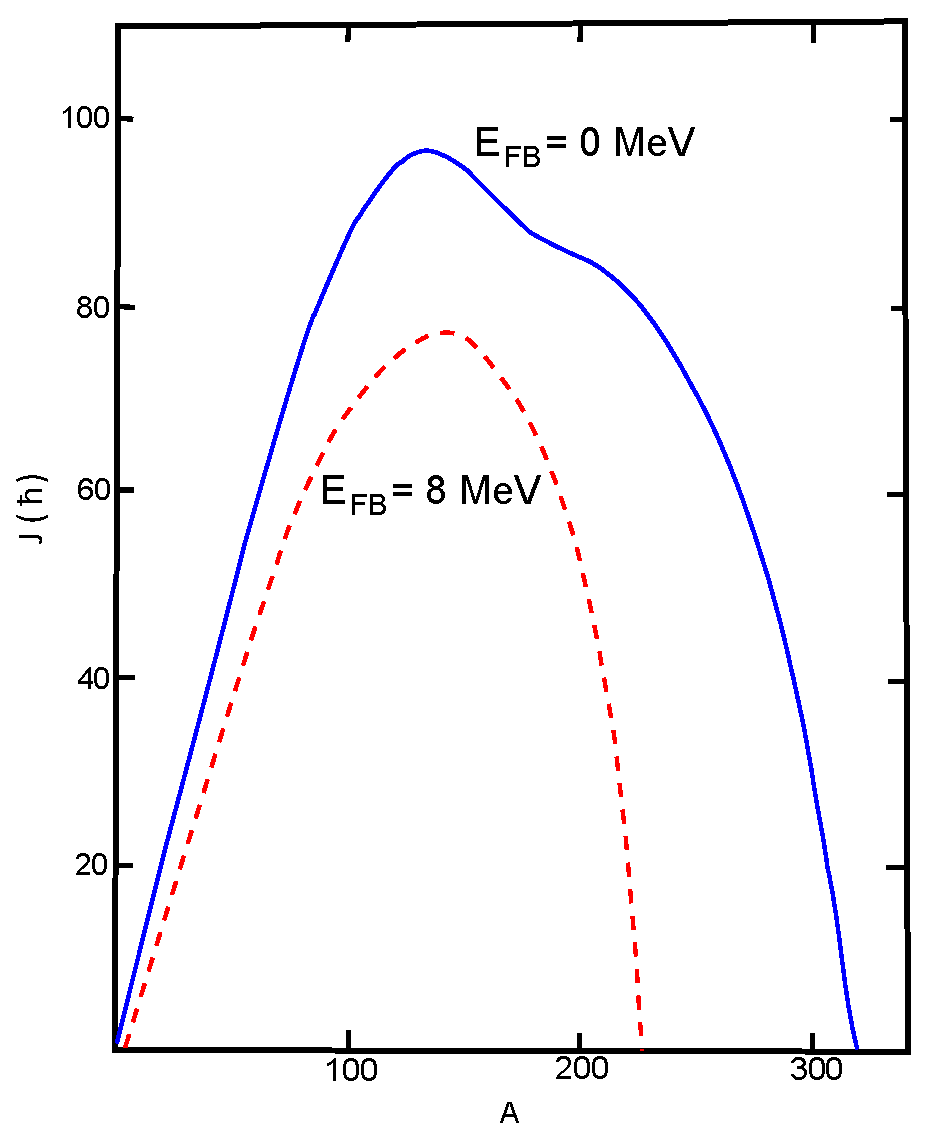
\includegraphics[height=0.3\textheight]{./img/c3/fission_barrier.eps}}
	\caption{Isocontours of angular momenta that yield fission barriers of $8MeV$ and $0MeV$ at various masses. Adapted from Ref. \cite{fissionBarrier2}.}
	\label{fig:chp3-fission-barrier}
\end{figure}

If the compound nucleus does not fission then it will instead evaporate particles. Particle evaporation is the emission of protons, neutrons, or alpha particles over or through an emission barrier. For charged particles this emission barrier is composed both of a centrifugal term which grows with increasing angular momentum and a coulomb term. For neutrons the emission barrier is solely the centrifugal barrier. As charged particles see a higher barrier due to the coulomb term, neutron evaporation is more probable in most cases. The exception occurs for very neutron deficient nuclei where the reduced proton separation energies make it possible for charged particle emission to compete with, or even dominate charged particle emission. Each successive evaporated particle carries energy, but little angular momentum away from the nucleus until there is insufficient excitation energy for particles to penetrate the emission barrier and the nucleus is left in a state that is stable against particle emission. From this point on the nucleus must dissipate its excess angular momentum and excitation energy via \gr{} emission. A schematic of this can be seen in Fig. \ref{fig:chp3-emission-schematic}.

\begin{figure}[h!]
	\centerline{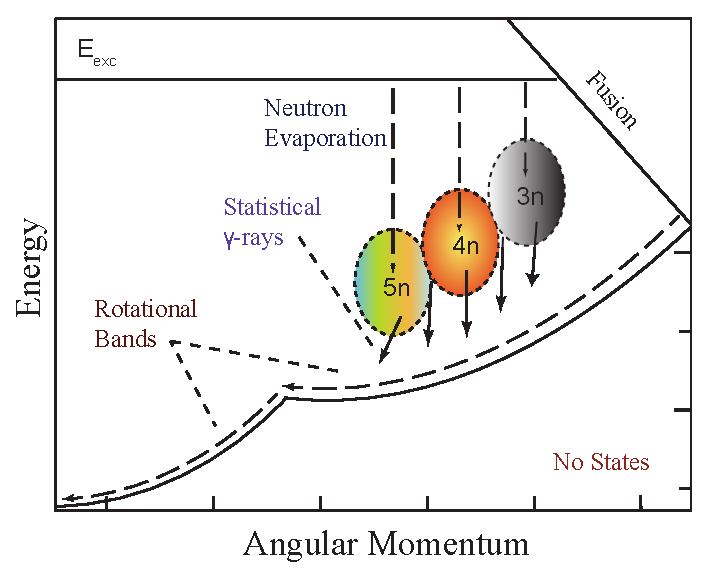
\includegraphics[height=0.3\textheight]{./img/c3/evaporation_chans.eps}}
	\caption{Schematic of the compound nuclear decay assuming that a rotational nucleus is being formed. Adapted from Ref. \cite{danielDissertation}.}
	\label{fig:chp3-emission-schematic}
\end{figure}

Initially the nucleus is in a state with such high level density that it decays by the emission of statistical \gr{}s\cite{cnCooling}. These statistical \gr{}s are almost purely dipole in nature and form a continuum as the notion of a discrete state is not a good one at such high level densities. As the nucleus approaches the yrast line (the states with the minimum excitation energy for a given angular momentum) the level density drops. This allows the emission sequences of discrete \gr{}s which feed the yrast line.

\subsection{Choice of Beam and Target}
\label{ssec:exp-pr-fus-evap-beam-target}
When choosing the beam and target for a fusion evaporation one must consider several factors: What is the production cross-section of the desired residual nucleus? How clean is the production of the desired residual nucleus relative to the other residuals? What is the spin range one wishes to study? What is the availability of the isotopes desired? What is the suitability of the material for beam production? While beam target combinations are usually chosen to maximize the cross-section for the desired residual, in some cases there are other channels open which will have large cross-sections themselves. In these cases the beam-target combination might be chosen to drastically lower the relative yield in competing channels at the cost of lowering the cross-section for the desired residual. For lower spins one usually chooses lighter projectiles. While Eqn. \ref{eqn:cn_lmax} clearly shows that it is possible to increase the angular momentum transfer with higher beam energies, this also increases the excitation energy of the compound nucleus, causing particle evaporation to be more probable. In the end, the decision is based on what combination yields the nucleus one wishes to study in the spins one wishes to study with the highest absolute and relative cross-sections possible.

Ref \cite{nucSpecAndReacPartC} gives the empirical estimate for $A_{CN}>100$ for obtaining the optimum beam energy for producing a specific residual nucleus in a (HI,xn) reaction which can be found in Eqn. \ref{eqn:fe_peak_selection}.
\begin{equation}
\label{eqn:fe_peak_selection}
E_{pk}(x)=(-Q_{x} + \alpha{}x)(1+\frac{A_p}{A_t})
\end{equation}
Here $Q_x$ is the Q-value for the production of the residual nucleus given by:
\begin{equation}
\label{eqn:res_qvalue}
Q = (M_t+M_p-M_{res}-x M_n)c^2
\end{equation}
and $\alpha$ is $\sim6MeV$. Of course, the reaction will only have a reasonable cross-section if $E_{pk}(x)$ is greater than $E_{CB}$, which is the height of the coulomb barrier, given in Eqn. \ref{eqn:cb_en}. In more modern times computer codes that employ statistical models such as PACE4\cite{PACE4,PACE4_2} can be used to calculate the cross-sections of products from these reactions allowing one to estimate peak beam energies and optimal beam-target combinations. A plot of cross-sections yielded by calculations such as these can be found in Fig. \ref{fig:chp3-pace4-calc}

\begin{figure}[h!]
	\centerline{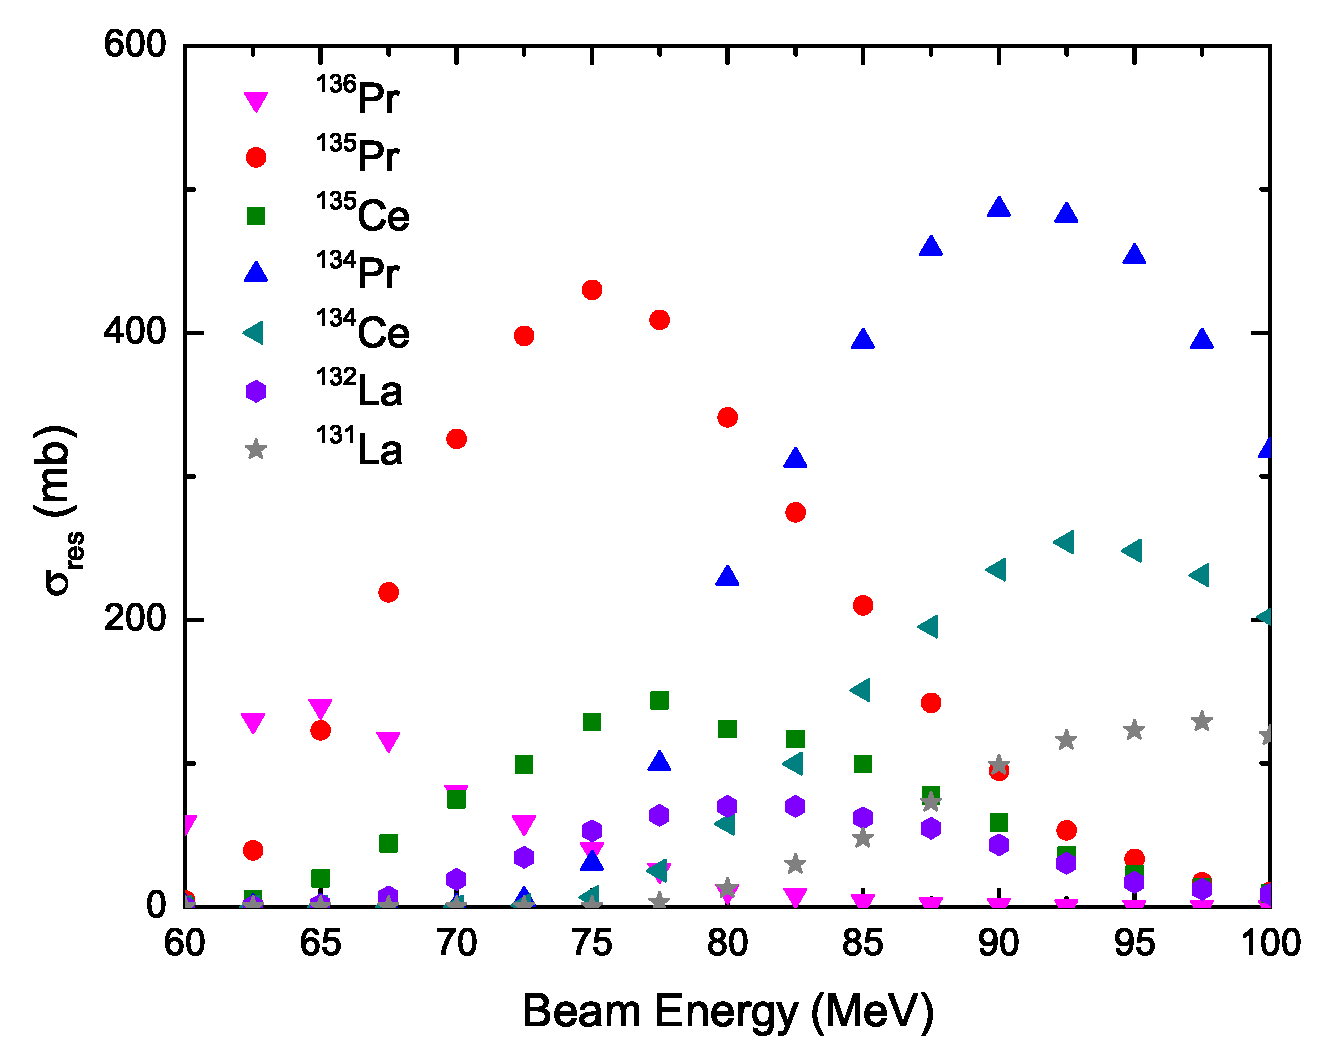
\includegraphics[width=\textwidth]{./img/c3/135Pr_calc_plot.eps}}
	\caption{Cross-sections of various residual nuclei for a $^{16}$O beam on $^{123}$Sb at a variety of beam energies as calculated by PACE4. As $^{139}$Pr is the compound nucleus produced all products that are not isotopes of Pr require the evaporation of a charged particle.}
	\label{fig:chp3-pace4-calc}
\end{figure}

\section{Gamma-ray Spectroscopy}
\label{sec:exp-pr-gamma-spec}
\subsection{Gamma-ray Interaction with Matter}
\label{ssec:exp-pr-gamma-spec-interactions}
As mentioned earlier, the choice of equipment will vary with which signals you need to collect to understand the system. In the case of a residual nucleus at high spin one of the obvious signal choices is the \gr{}s it emits. Detection of gamma-rays is dependent on the \gr{} depositing energy in a detector which in turn depends on the interactions of electromagnetic radiation with matter. At the energies relevant to nuclear physics, $10keV<E_{\gamma}<15MeV$, there are three primary processes to be considered, photoelectric absorption, Compton scattering, and pair production. These three processes compete with each dominating in a different energy range.

In photoelectric absorption the photon interacts with a bound electron in the detector material and is fully absorbed\cite{einstein-PE}. The total energy of the photon is then used to overcome the binding energy of the electron and to provide the electron with kinetic energy, giving $E_{e^-}=E_{\gamma}-E_b$. The electron then proceeds to lose energy as it passes through the detector material. In \gr{} spectra the full energy peak corresponds to the deposition of the photon's full energy in the detector medium. For that to occur either the primary photon, or all the secondary photons (generated by the processes below), must undergo photoelectric absorption. As can be seen in Fig. \ref{fig:chp3-gamma-interactions} the photoelectric effect is dominant at low energies and the energy at which the photoelectric effect ceases to dominate increases with the Z of the material.

\begin{figure}[h!]
	\centerline{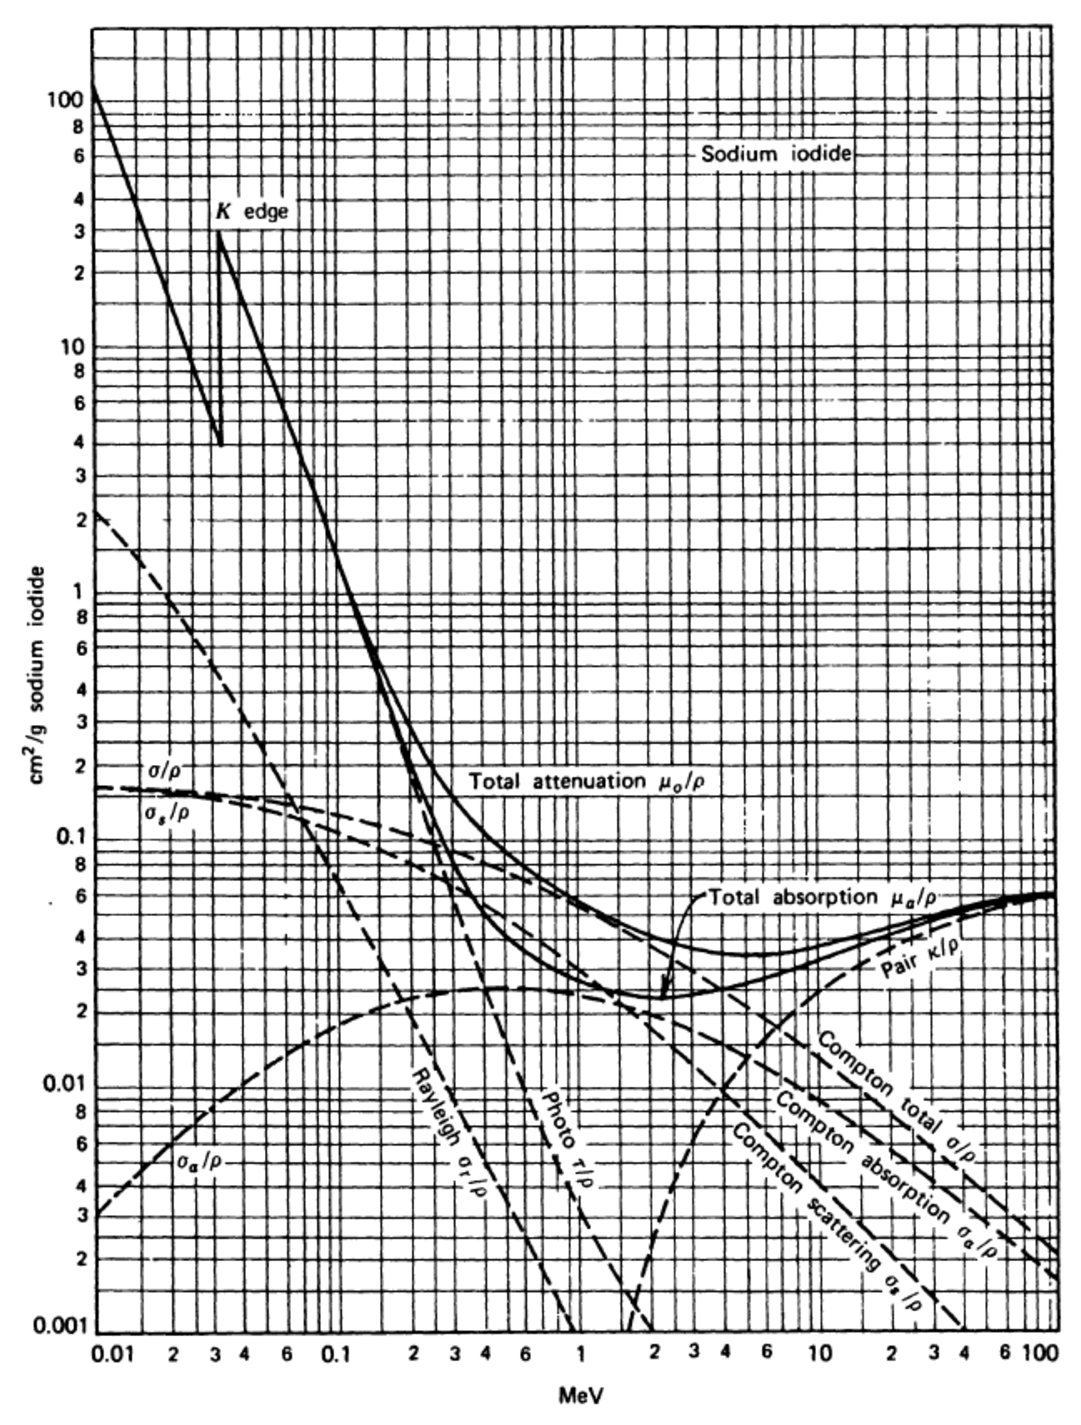
\includegraphics[height=0.5\textheight]{./img/c3/gamma_interactions_scan.eps}}
	\caption{Gamma-ray attenuation coefficients for various processes in NaI, adapted from Ref. \cite{knollBook}. Here we can see the dominance of photoelectric absorption at lower energies, Compton scattering at intermediate energies and pair production at high energies. While the slopes of these processes changes from material to material the trends remain the same.}
	\label{fig:chp3-gamma-interactions}
\end{figure}

In Compton scattering, a \gr{} photon scatters from an electron in the material at some angle $\theta$ to its original direction\cite{Compton-PhysRev.21.483}. Due to conservation of momentum and energy, the energy transferred to the electron is precisely determined by $\theta$ and so the energy of the secondary photon can be written as: $E_{s}=E_{p}(1+\frac{E_{p}}{m_{e}c^2}(1-Cos\theta))^{-1}$ As above the electron then deposits its kinetic energy in the medium as it slows. However, unlike in the photoelectric effect, not all of the energy is deposited in the electron. After the scattering the secondary photon travels in its new direction and is free to interact again with probabilities dictated by its energy. As shown in Fig. \ref{fig:chp3-gamma-interactions} Compton scattering is the dominant effect at intermediate energies.

The final process to be considered is pair production. In pair production the photon enters the region of very strong electric field near the nucleus and its energy is converted into the mass and kinetic energy of an electron positron pair \cite{anderson-PhysRev.43.491,oppenheimer_PhysRev.44.53.2}. Since energy is conserved the photon must have energy of at least twice the rest mass of the electron, giving a threshold of $E_{\gamma}\geq1.022MeV$ for this interaction, any energy above this threshold is converted into kinetic energy shared between the two particles. After their production the electron and positron will both travel through the detector medium loosing energy as they travel. Once at rest the positron will annihilate with an electron, emitting two anti-parallel $511keV$ secondary photons. Fig. \ref{fig:chp3-gamma-interactions} shows the dominance of this interaction at high gamma energies, the energy at which pair production supersedes Compton scattering decreases with increasing Z of the material.

\subsection{High Purity Germanium (HPGe) Detectors}
\label{ssec:exp-pr-gamma-spec-hpge}
In detecting gamma-rays there are essentially 3 major classes of detector, scintillator, gas, and semiconductor detectors. In all cases the \gr{} enters the active volume of the detector and deposits energy by at least one of the processes mentioned above, the primary energetic electrons, produced directly by the interactions of the \gr{}, then proceed to ionize or excite other electrons in the material, the secondary electrons are then detected in some manner. In scintillators they cause UV or visible light to be emitted and that is collected via photomultiplier or similar to produce a voltage pulse. In gas and semiconductor detectors the charge of the secondary electrons (and their corresponding ions or holes) is collected directly, albeit via different mechanisms, to produce the voltage pulse.

It is desirable that \gr{} detectors have both good detection efficiency and energy resolution. Unfortunately, in the \gr{} detectors presently available there is a conflict between these goals and so one must decide which parameter is more important. For high spin experiments where the spectrum is dense with peaks the energy resolution is the top priority as broad peaks would be indistinguishable from each other. Amongst the available detectors, semiconductor detectors, particularly High Purity Germanium (HPGe) detectors offer the best energy resolution.

Semiconductor detectors are reversed bias diodes with either a p-n or a p-i-n junction. At the boundary between the types of materials there is a so called contact potential. This potential gives rise to an electric field which causes the migration of charges between the two materials until there is an area bridging the boundary called the depletion zone. In this zone there is an electric field which gives rise to a potential that counters the contact potential. By applying reverse bias to the diode the contact potential is effectively increased causing the depletion zone to expand (schematic in Fig. \ref{fig:chp3-pn_diode}.) This is desirable because the depletion zone(s) are the only regions of the semiconductor where an electric field will exist. This means that electron hole pairs formed in the within it are swept away from each other before they can recombine so that they can be collected. In contrast, electron hole pairs formed outside the depletion zone are not pulled away from each other and recombine, preventing their collection. Due to this, the depletion zone of the detector is the region that is active. That is to say that the passage of ionizing radiation through the that region is detectable as electron hole pairs it produces will be collected.

\begin{figure}[h!]
	\centerline{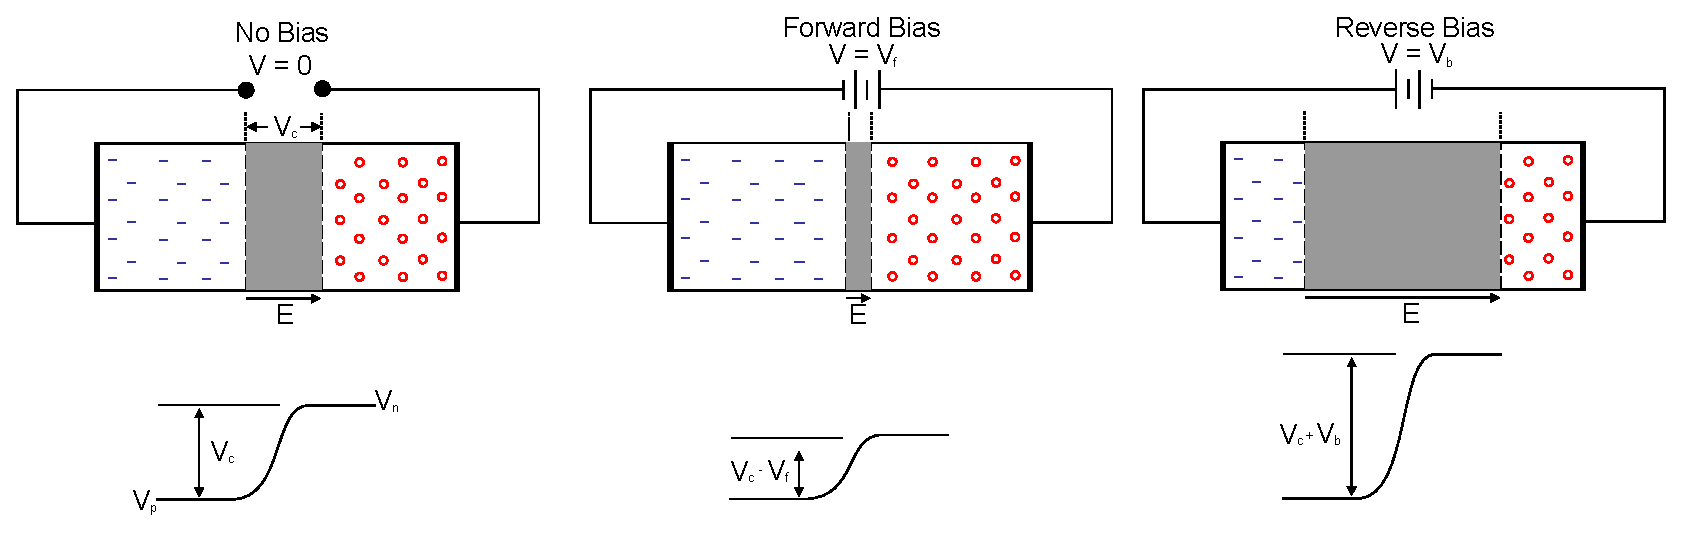
\includegraphics[width=\textwidth]{./img/c3/pn-diode.eps}}
	\caption{Above: Diagramatic view of the depletion zone's with varying bias voltage. Below: Voltage difference across the depletion zone for each bias voltage shown above}
	\label{fig:chp3-pn_diode}
\end{figure}

The higher the purity of the semiconductor, the higher the reverse bias voltage that can be applied without reaching the breakdown of the semiconductor (usually catastrophic event.) In HPGe detectors the purity is sufficiently high that the whole crystal of Ge can be depleted yielding a very large active region, an advantage for \gr{}s given their low interaction probabilities compared to charged particles. When a gamma interacts in an HPGe detectors it produces at least one high energy secondary electron or positron (more if there are multiple interactions). These secondary electrons lose energy quickly as they pass through the detector, leaving a trail of electron hole pairs in their wake. The electrons and holes are then swept to their respective contacts by the applied potential and collected.

A detectors resolution is defined the FWHM for a given peak. The intrinsic resolution of a semiconductor detector stems from statistical fluctuations in how many electrons and holes are collected at the terminals. As these fluctuations arise from simple counting statistics one their form can be deduced to be:
\begin{equation}
\label{eqn:hpge-res-est} 
\Delta{}E_{in} \propto \frac{E_{\gamma}}{\sqrt{N}}
\end{equation}
Where N is the number of charge carriers produced and is approximately $E_{\gamma}/\epsilon$ where $\epsilon$ is the average energy to make an electron hole pair ($2.96eV$ for Ge). In a more careful examination we see that the intrinsic component of the FWHM is:
\begin{equation}
\label{eqn:hpge-in-res} 
\begin{split}
\Delta{}E_{in}(E) & = 2\sqrt{2 ln(2)}\frac{\sqrt{F E_{\gamma{}}/\epsilon{}}}{E_{\gamma{}}/\epsilon{}}E_{\gamma{}}\\
       & = 2.355\sqrt{F\epsilon{}E_{\gamma{}}}
\end{split}
\end{equation}
Here $F$ is the Fano factor. This value, intrinsic to the detector material, ranges across $(0,1]$ and takes into account energy loss mechanisms available to the secondary electron(s) that do not generate electron hole pairs. The inquiring reader can find a more thorough explanation in Refs. \cite{knollBook,fano_factor1}.

Unfortunately, the detector's intrinsic resolution is not the only contributor to the detector's resolution. There are also contributions from such sources as electronic noise, charge carrier collection / trapping, and Doppler broadening. If one assumes that these components are independent and normally distributed one gets the actual resolution to be:
\begin{equation}
\label{eqn:hpge-res} 
\Delta{}E_{T}^2 = \Delta{}E_{in}^2 + \Delta{}E_{E}^2 + \Delta{}E_{C/T}^2 + \Delta{}E_{D}^2
\end{equation}
Where $\Delta{}E_{E}$ is the electronic noise contribution, $\Delta{}E_{C/T}$ is the charge collection / trapping term, and $\Delta{}E_{D}$ is the Doppler broadening term. Ref. \cite{trappingResolution} gives the FWHM forms of the noise and collection / trapping terms to be:
\begin{equation}
\label{eqn:hpge-res-noise} 
\Delta{}E_{E} = N_{1/2}
\end{equation}
\begin{equation}
\label{eqn:hpge-res-ct} 
\Delta{}E_{C/T} = 2.355\sqrt{\epsilon{} K E_{\gamma{}} [1-\eta{}(r)]}
\end{equation}
Where $N_{1/2}$ is the FWHM of the electronic noise, $K$ is a constant of a given detector, and $\eta{}(r)$ is the total charge collection efficiency of electrons and holes of the detector as a function of the interaction site's radius.

\begin{figure}
	\centerline{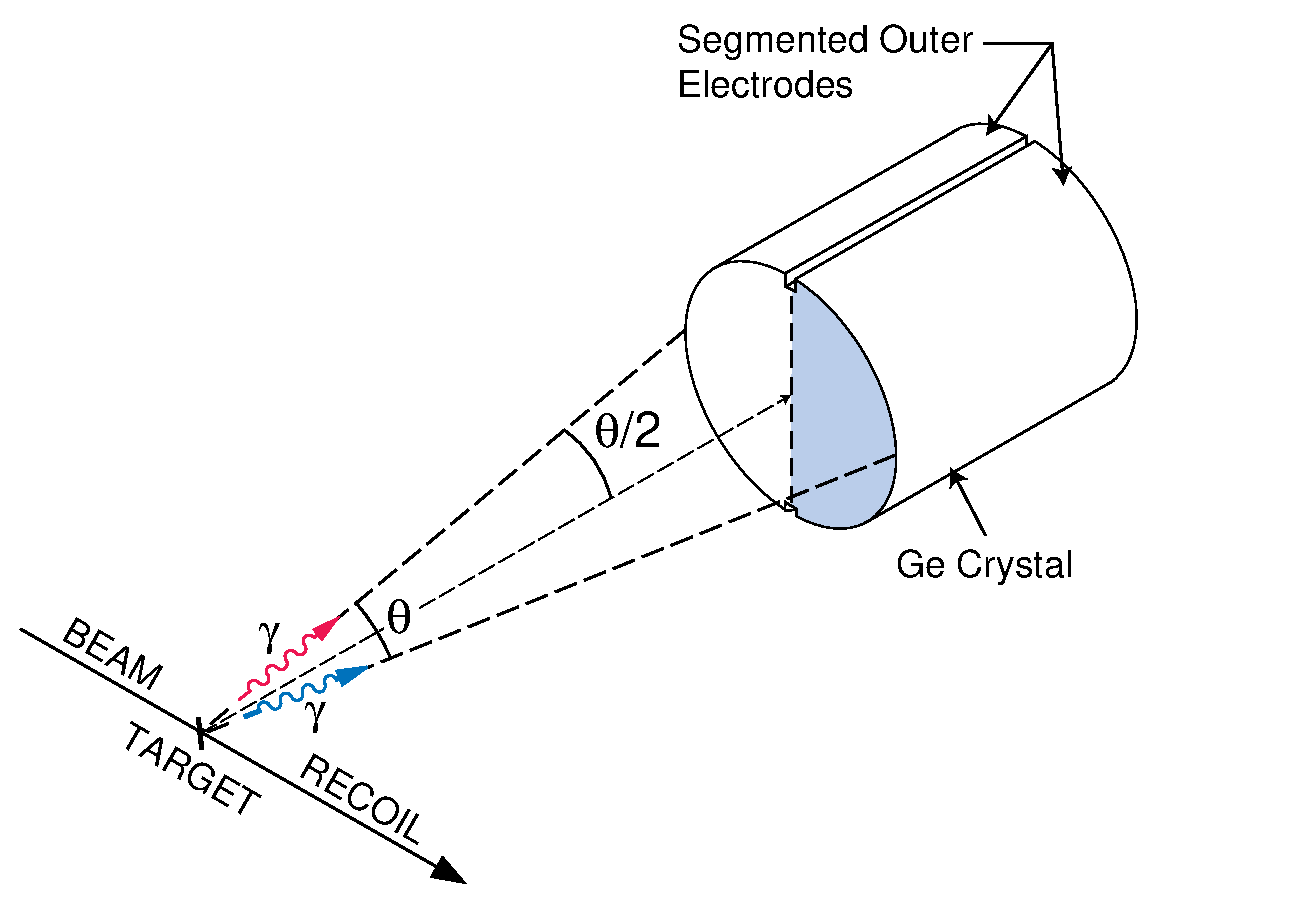
\includegraphics[height=0.3\textheight]{./img/c3/split_contact.eps}}
	\caption{Diagram showing the uncertainty inherent in the \gr{}'s angle of emission, as well as Gammasphere's segmented electrode scheme to reduce this.}
	\label{fig:chp3-doppler-split-contact}
\end{figure}

The final term, $\Delta{}E_{D}$, of this equation comes from uncertainty in the angle at which the gamma ray was emitted from the recoiling nucleus due to the detectors finite size (shown in Fig. \ref{fig:chp3-doppler-split-contact}.) The shift in gamma energy due to the nuclear recoil is:
\begin{equation}
\label{eqn:doppler_formula} 
E_{o} = E_{e}\frac{\sqrt{1+\beta{}Cos(\theta)}}{\sqrt{1-\beta{}Cos(\theta)}}
\end{equation}
here, the subscripts o and e refer to observed and emitted, $\beta$ is the speed of the recoiling nucleus and theta is the angle between the nucleus' line of a flight and the emitted \gr{}. If the detector has an angular acceptance such that $\theta{}_{0}-\delta{}\theta{}\leq{}\theta{}\leq{}\theta{}_{0}+\delta{}\theta{}$ with $\theta{}_{0}$ the central angle of the detector; we find that, to first order, the contribution of Doppler broadening is:
\begin{equation}
\label{eqn:res-doppler-term} 
\Delta{}E_{D} = 2\beta{}Sin(\theta{})Sin(\delta{}\theta{})E_{\gamma}
\end{equation}
There are three strategies to combat this term. The first is geometrical. By increasing the granularity of the array, either by using more, smaller detectors, or by using more detectors at a longer distance from the source. This in turn would shrink the opening angle of detectors and therefor reduce the Doppler broadening. The second method is electrical in nature, by segmenting the outer contact of the detector, even roughly, one can localize within the detector where the interaction occurred, therefor effectively reducing the opening angle. Gammasphere uses this strategy as shown in Fig. \ref{fig:chp3-doppler-split-contact}. The split outer contact lets one reduce the effective opening angle, $2\delta{}\theta{}$, from $14.9^{\circ}$ to $7.45^{\circ}$ \cite{TheGS}. The third method involves a physical segmentation of the detector, by having multiple crystals in close proximity within the same cryostat. This, give a detector that has a volume equal to the sum of the individual crystal volumes.However the opening angle of the individual crystals is the opening angle to consider for the Doppler broadening. Thus a physically segmented detector can give you a smaller Doppler broadening than an unsegmented detector of the same volume.  Clover and cluster detectors\cite{cloverDet,clusterDetector} are examples of this strategy.

\subsection{Escape Suppression with BGO detectors}
\label{ssec:exp-pr-gamma-spec-escape-supress}
The primary contribution to the background in \gr{} spec is the incomplete deposition of energy in the detector. Two of the mechanisms discussed in section \ref{ssec:exp-pr-gamma-spec-interactions} can lead to this. Compton scattering will result in incomplete energy deposition when the secondary photon yielded by the process may escape the HPGe crystal without depositing the rest of its energy. This mode results in a smooth background from the maximum energy transferable to an electron in the process down to zero energy. Pair production will yield incomplete energy deposition when one or both of the photons from the annihilation of the positron escape the detector. This mode results in 2 new peaks forming, the first $511keV$ below the photopeak, corresponding to one annihilation photon escaping, and a second $1022keV$ below the photopeak, corresponding to both escaping.
\begin{figure}[h!]
	\centerline{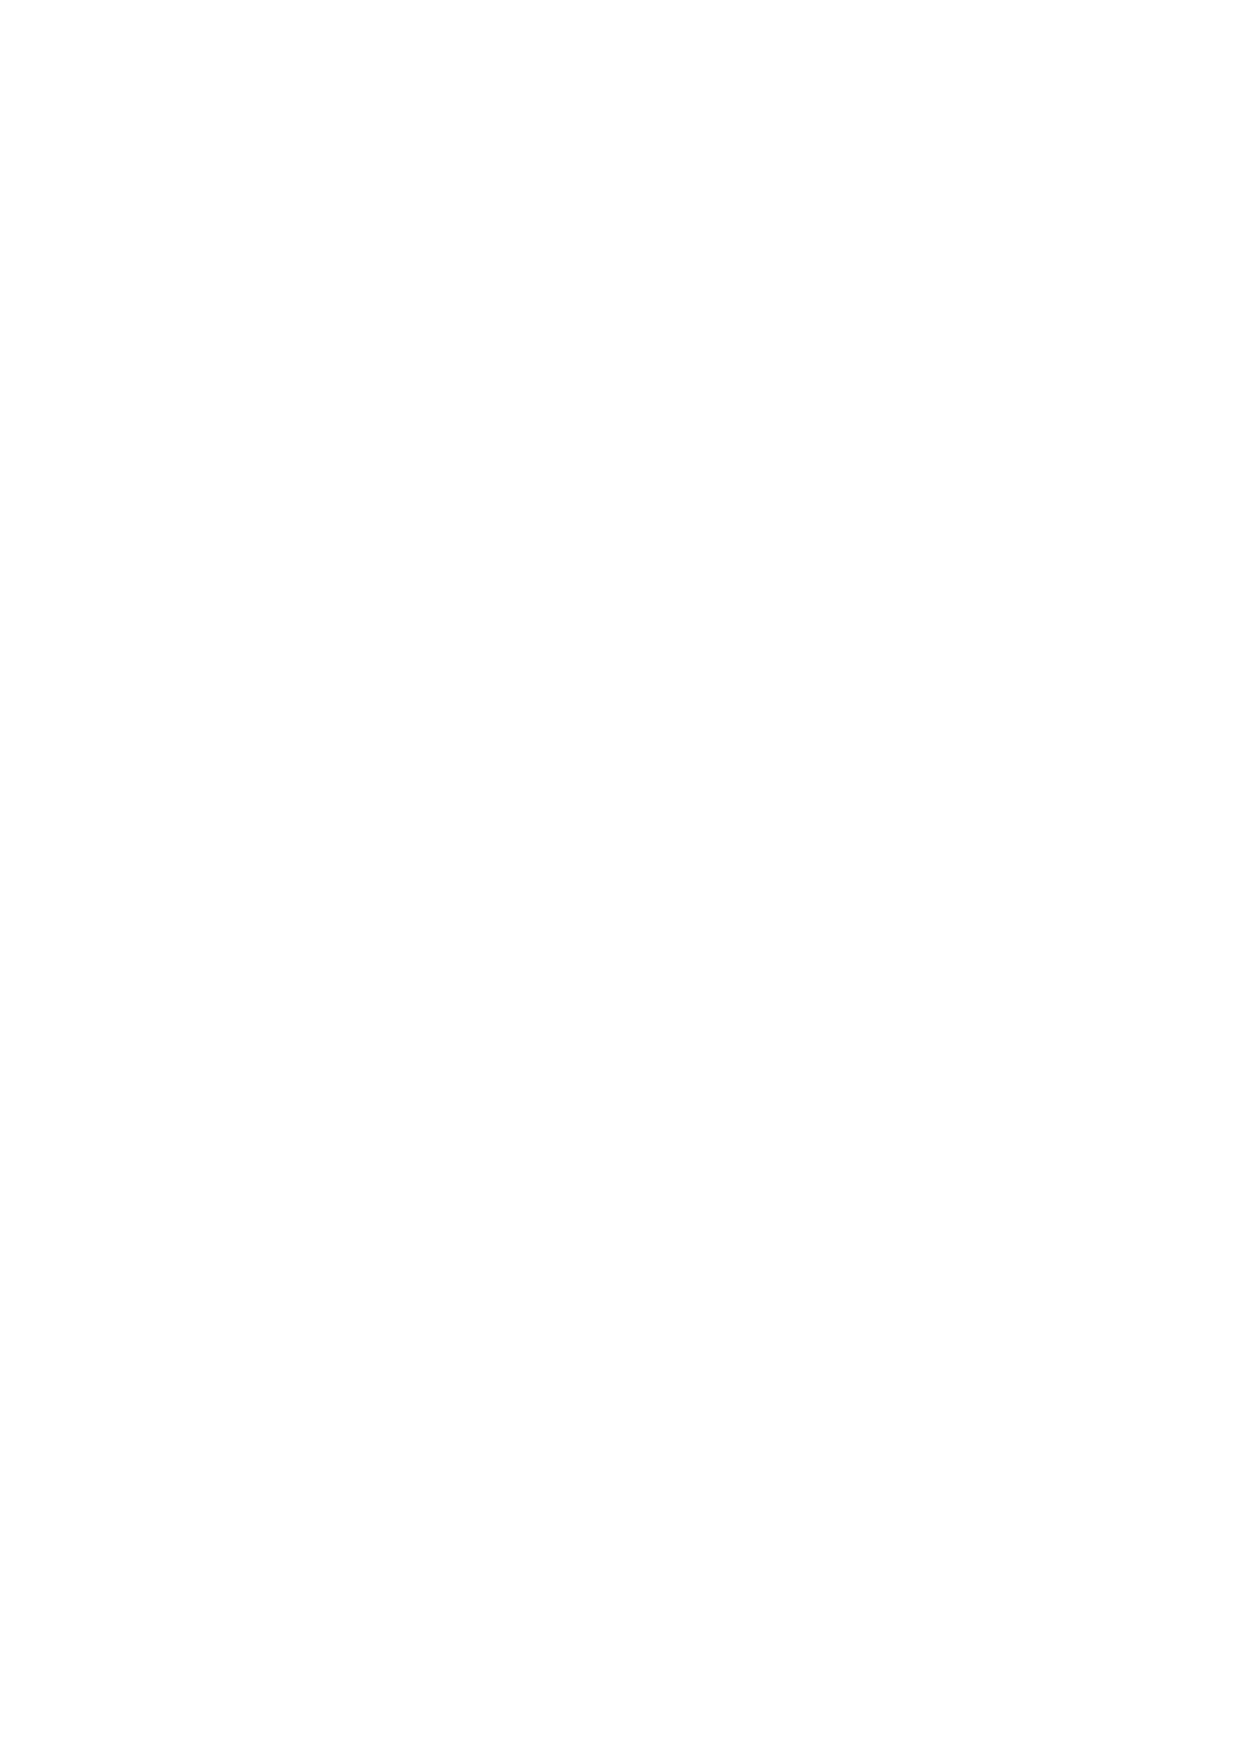
\includegraphics[height=0.25\textheight]{./img/c3/BGO_schematic.pdf}}
	\caption{Schematic of BGO escape suppression around an HPGE crystal.}
	\label{fig:chp3-supression-schematic}
\end{figure}
\begin{figure}[h!]
	\centerline{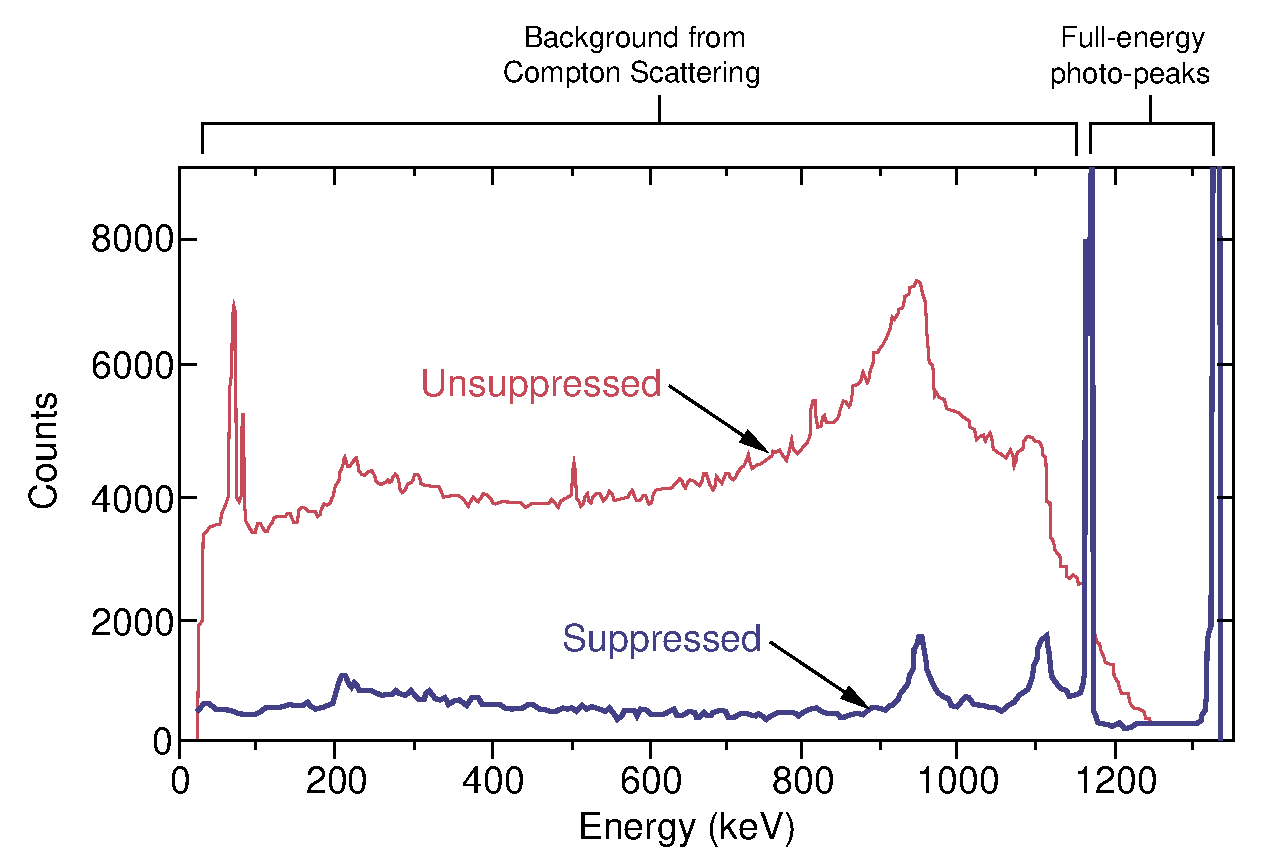
\includegraphics[height=0.25\textheight]{./img/c3/suppressed_spectra.eps}}
	\caption{Superimposed spectra of an escape suppressed and unsuppressed detector. Adapted from Ref.\cite{gsBooklet}}
	\label{fig:chp3-supression-improvement}
\end{figure}
To ameliorate this the principal detector is surrounded by a secondary detector and the electronics are set to be in anti-coincidence (see Fig. \ref{fig:chp3-supression-schematic} for a schematic.) If both detectors had energy deposited, the event is discarded.In practical application, the second detector must be highly efficient at detecting gammas so that it need not be overly large. Given this constraint, the scintillator Bismuth Germanate (BGO) is an excellent choice for escape suppression. While BGO's energy resolution is quite poor, it has excellent timing characteristics, quite high density, and is made of fairly high $Z$ materials. The latter two facts grant it the desired high detection efficiency (substantially higher than the HPGe it is shielding in fact.) Improvements up to a factor of $2.48$ in the peak-to-total ratio (P/T) can be seen for some designs. A bare HPGE detector having a (P/T) of $0.270\pm0.002$ has been see to improve to $0.669\pm0.002$\cite{GSComptonSuppression} with a escape suppression shield around the sides and part of the back (some space needs to be left for cables to exit the HPGe.) Example spectra showing this improvement can be seen in Fig. \ref{fig:chp3-supression-improvement}.

\subsection{The Gammasphere Detector Array}
\label{ssec:exp-pr-gamma-gammasphere}
Gammasphere (partially pictured in Fig. \ref{fig:chp3-gs-hemisphere}) is an array of $110$ escape suppressed HPGe detectors arranged in a sphere around a target. A cross sectional view of part of the array can be seen in Fig. \ref{fig:chp3-gs_det_schem}. The BGO shields are arranged in hexagonal shapes around each detector plus a backplug covering the majority of behind the detector. Gammasphere's spherical geometry is comprised of 17 rings of detectors, each ring at a distinct angle to the beam axis. Using a scheme called honeycomb suppression, Gammasphere has a total efficiency of $~0.09$ at $1MeV$ and a singles P/T of $0.69$.

\begin{figure}[h]
	\centerline{\includegraphics[height=0.3\textheight]{./img/c3/gammasphere_hemi.jpg}}
	\caption{View of scattering chamber and interior of one of Gammasphere's hemispheres drawn back from the chamber. The hexagonal copper foils are x-ray absorbers.}
	\label{fig:chp3-gs-hemisphere}
\end{figure}


\begin{figure}[h]
	\centerline{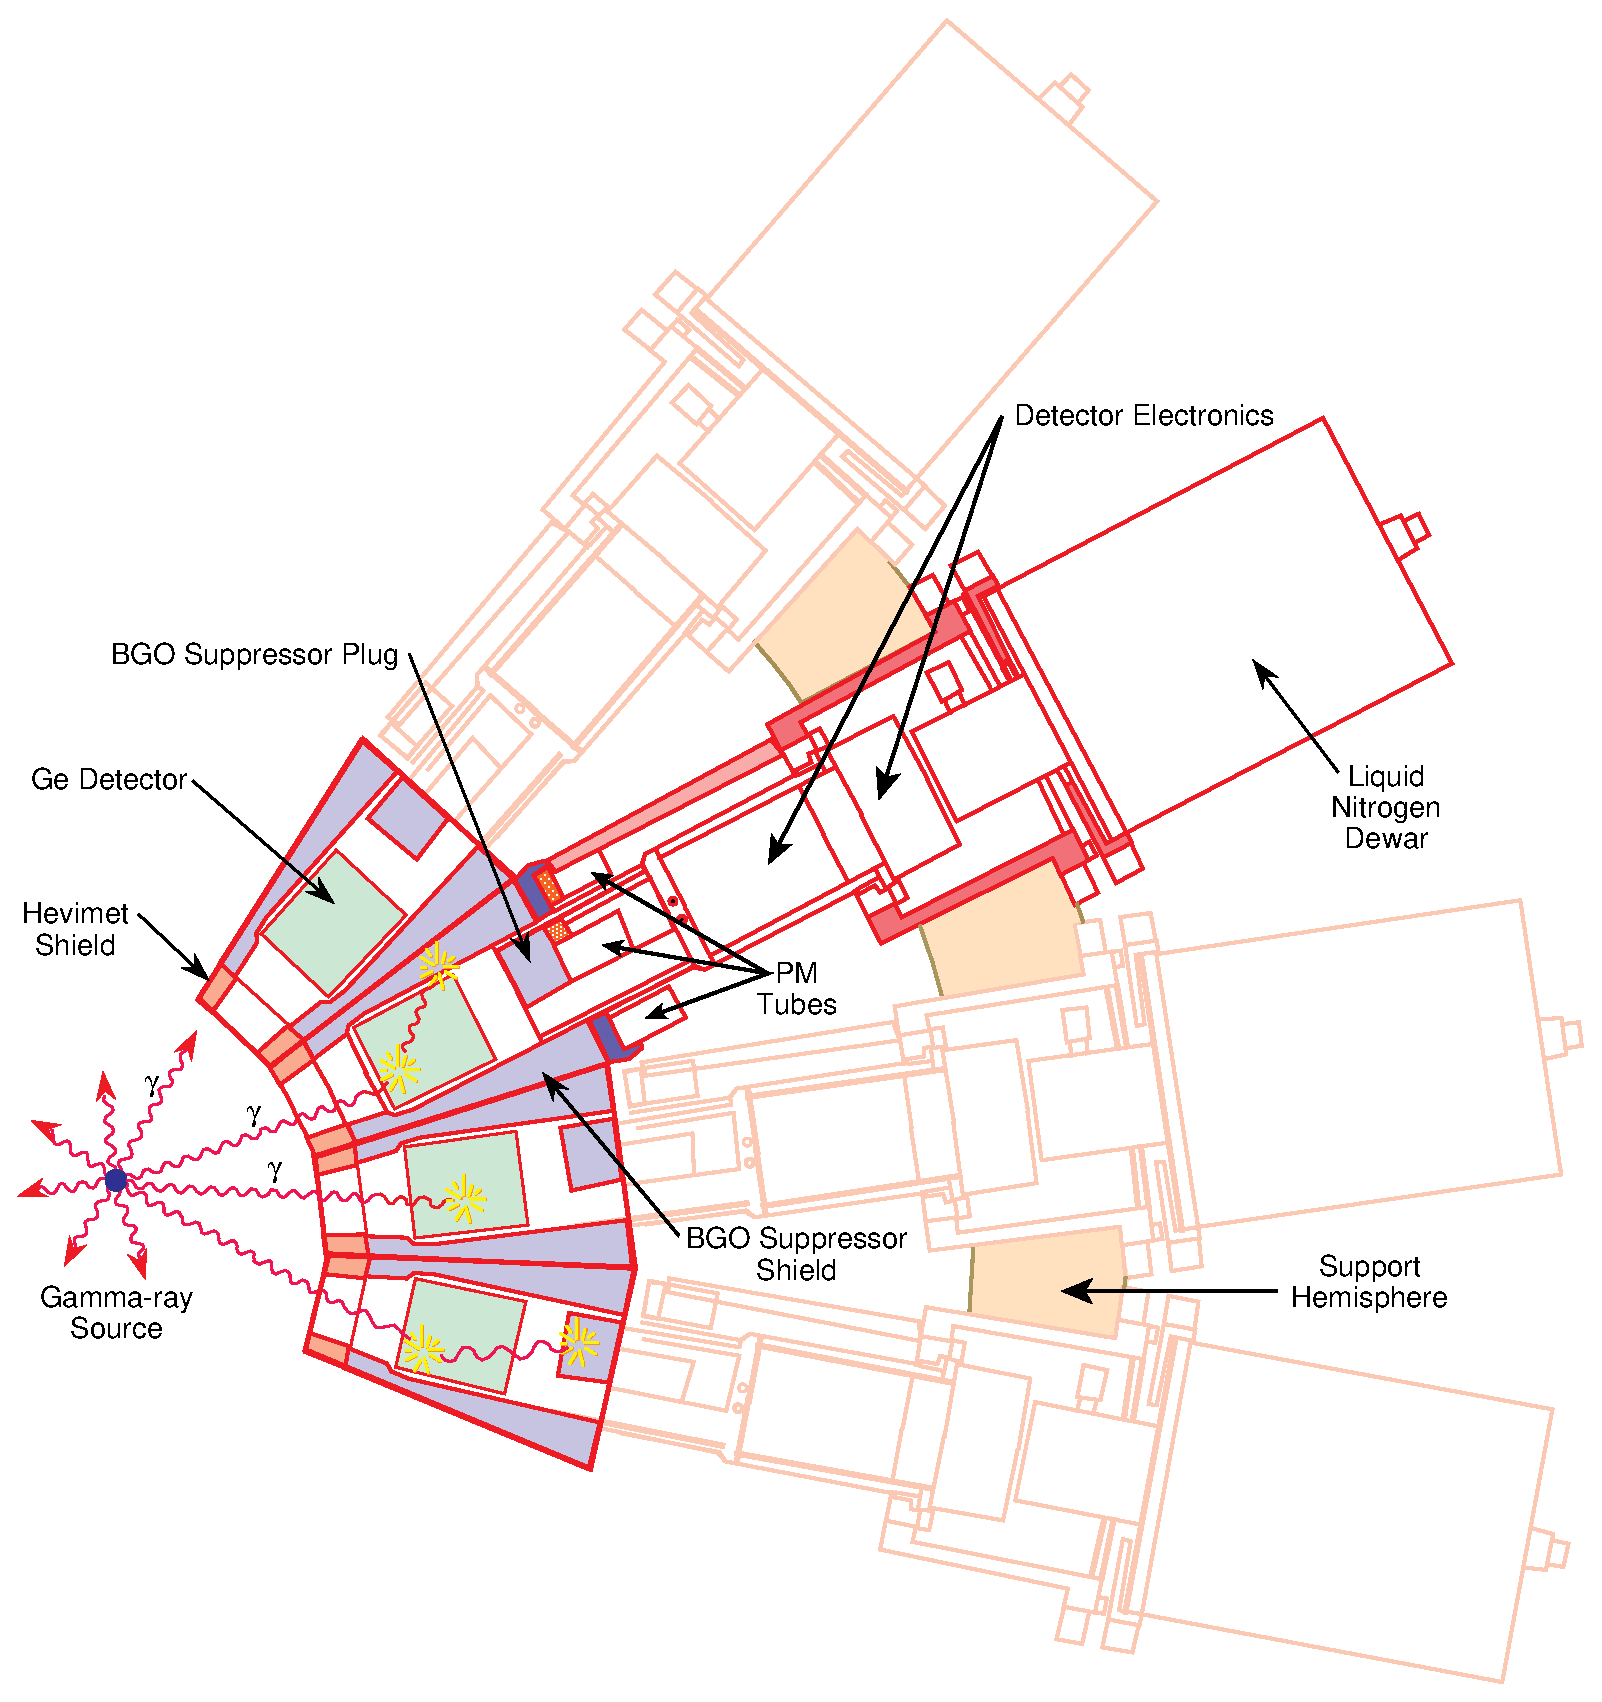
\includegraphics[height=0.3\textheight]{./img/c3/gammasphere_detector.eps}}
	\caption{Cross-section schematic of part of Gammasphere. Adapted from Ref.\cite{gsBooklet}}
	\label{fig:chp3-gs_det_schem}
\end{figure}


Honeycomb suppression is an escape suppression scheme that uses the BGO shields of adjacent detector modules to effectively double the thickness of a detector's shields. As seen in Fig. \ref{fig:chp3-gs_det_schem} almost every module will have additional modules immediately adjacent to it. If the HPGe detector for a given module do not register energy deposition the 6 side segments of its BGO shield are used to double the thickness of the shields they are adjacent to. Without this measure the singles P/T is $\sim0.62$; using honeycomb suppression improves this to $\sim0.69$ though it reduces the total efficiency at 1.332MeV from $\sim0.095$ to $\sim0.089$\cite{TheGS}. Table \ref{tbl:gs-summary} contains a brief summary of Gammasphere's features drawn from Refs. \cite{TheGS,SimulatedResGS,GSComptonSuppression,largeArrays}.

\begin{table}[h]
\caption{GAMMASPHERE FEATURE SUMMARY\label{tbl:gs-summary}}
\begin{center}
\begin{tabular}{|c|c|}
\hline
\hline No. Detectors             & 110 \\ 
No. Segmented Detectors   & 70 \\ 
HPGe Detector Size        & $7.1 cm$ (D) $\times$ $8.22 cm$ (L) \\
Detector Volume           & $312.8 cm^3$\\
Target to HPGe Front      & $24.6 cm$\\ 
Total HPGE Solid Angle    & $0.46 \times 4\pi$\\ 
Total Peak Efficiency     & $0.094$ at $1.3 MeV$\\ 
Singles P/T               & $0.6$ at $1.3 MeV$ \\ 
Energy Resolution (MeV)   & $2.1keV$ at $1.3 MeV$ \\ 
\hline 
\hline 
\end{tabular}
\end{center}
\end{table}

As mentioned in section \ref{ssec:exp-pr-gamma-spec-hpge} some of Gammasphere's detectors have a split outer electrode to reduce the effective half angle. Detector positions can be found in table \ref{tbl:app1-gs-rings} and table \ref{tbl:app1-gs-detectors} in appendix \ref{app:gs-rings-and-detectors}. Gammasphere's high granularity, good energy resolution, and efficiency make it a boon for high \gr{} multiplicity coincidence measurements.

\subsection{Indian National Gamma Array (INGA)}
\label{ssec:exp-pr-gamma-spec-inga}
The Indian National Gamma Array (pictured in Fig. \ref{fig:chp3-INGA}) is an array of 24 escape suppressed HPGe clover detectors\cite{ingaAtIUAC}. Since INGA utilizes clover detectors it is sensitive to the polarization of \gr{} emitted from nuclei in aligned states\cite{cloverDet}. Additionally, the use of clover detectors make the array more efficient for high energy \gr{} when using add back mode.

\begin{figure}[h!]
	\centerline{\includegraphics[height=0.25\textheight]{./img/c3/INGA.JPG}}
	\caption{Exterior view of INGA.}
	\label{fig:chp3-INGA}
\end{figure}

INGA's current incarnation utilizes a digital data acquisition system (DAQ) that allows it to run in a triggerless mode producing timestamped gamma data from a $10ns$ clock\cite{IngaDigitalDAQ}. Digital data acquisition systems, because they digitize the preamp signal directly, can operate at higher counting rates than analog because they do not require multiple microseconds of signal shaping time. The downside of this mode, is that coincidence are not prebuilt by the DAQ and instead need to be constructed by moving a sliding window of the desired coincidence time across the timeline of events and selecting sets of gammas that occur within that window. A final advantage of the time stamped events is that isomers can have their lifetime measured using time differences between \gr{}s as seen in Fig. \ref{fig:chp3-INGA-isomer}

\begin{figure}[h!]
	\centerline{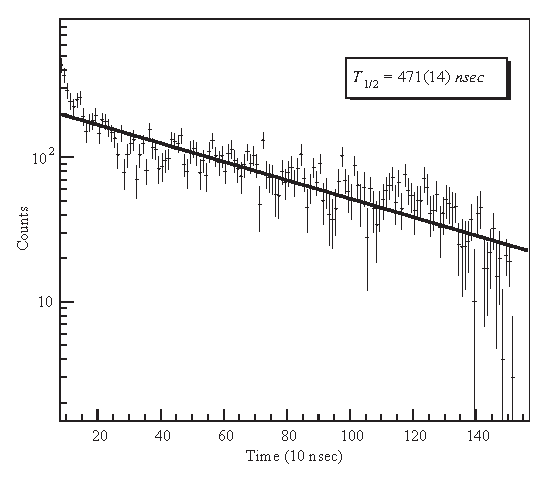
\includegraphics[height=0.35\textheight]{./img/c3/INGA_isomer.eps}}
	\caption{Example isomer timing spectrum for INGA. From Ref. \cite{IngaDigitalDAQ}.}
	\label{fig:chp3-INGA-isomer}
\end{figure}

Using its digital DAQ and add-back on the clover crystals, INGA achieves a total efficiency of $\sim0.05$ and P/T of $0.4$ at $\sim1.33MeV$. Table \ref{tbl:inga-summary} contains summary of INGA's features. INGA's sensitivity to polarization, efficiency, and granularity make it a good system for intermediate \gr{} multiplicity coincidence measurements, reaching its best efficiency at 2- to 3-fold events.

\begin{table}[h]
\caption{INGA FEATURE SUMMARY\label{tbl:inga-summary}}
\begin{center}
\begin{tabular}{|c|c|}
\hline
\hline
No. Clover Detectors      & 24\\ 
No. Single Crystals       & 96\\ 
Single Crystal Size       & $5 cm$ (D) $\times$ $7 cm$ (L) \\
Single Crystal Volume     & $117.5 cm^3$\\
Target to HPGe Front      & $24 cm$\\ 
Total HPGE Solid Angle    & $0.25 \times 4\pi$\\ 
Total Peak Efficiency     & $0.05$ at $\sim1.0 MeV$\\ 
Singles P/T               & $0.40$ at $1.3 MeV$ \\ 
Energy Resolution (MeV)   & $2.2keV$ at $1.3 MeV$ \\ 
\hline 
\hline 
\end{tabular}
\end{center}
\end{table}

\section{Experimental Details}
\label{sec:exp-pr-details}
The work on \pr{} presented in this dissertation was performed at two different facilities, the ATLAS (Argonne Tandem Linear Accelerator System) facility with the Gammasphere detector system, and the TIFR-BARC Pelletron LINAC with the INGA detector system. At both facilities the $^{16}O(^{123}Sb,4n)^{135}Pr$ reaction was used. As mentioned in section \ref{sec:exp-pr-fus-evap} the choice of beam and target affects both the most probable channel, the excitation energy, and the maximum angular momentum of the compound (and residual) nucleus. In previous in-beam \gr{} spectroscopy literature the following heavy ion fusion evaporation reactions have been used to reach yield the \pr{} residual nucleus: $^{120}Sn(^{19}F @ 91MeV,4n)^{135}Pr$\cite{Semkow135Pr}, $^{123}Sb(^{16}O @ 76MeV,4n)^{135}Pr$\cite{135PrLifetimes}, and  $^{116}Cd(^{23}Na @ 115MeV,4n)^{135}Pr$\cite{EPaul135Pr}. The $^{16}$O and $^{123}$Sb projectile-target combination was chosen for its lighter projectile to optimize for the population of states further from the yrast line.

\subsection{ATLAS/Gammasphere}
\label{ssec:exp-pr-details-gs}
ATLAS is located at the Physics Division at Argonne National Laboratory in Argonne, Illinois, USA. ATLAS is the world's first superconducting ac linear accelerator (linac) for projectiles heavier than an electron and consists of 3 sections. The first of these sections is the injector accelerator which can be either a 9 Megavolt (MV) tandem Van de Graff accellerator or an electron cyclotron resonance (ECR) ion source coupled to a 12 MV low velocity LINAC (PII, Positive Ion Injector). The beam from the chosen injector is sent the 20 MV ``booster'' linac and finally to the 20 MV ``ATLAS'' linac. This system produces pulsed beams with spot diameter $\leq1mm$, pulse length $\leq500ps$, and interval $82ns$ which range across all elements from hydrogen to uranium with energies of $7-17MeV$ per nucleon ($/\mu{}$.)

The Gammasphere detector system was used in the FMA (Fragment Mass Analyzer) position though the FMA itself was not used. This configuration requires that the first ring of detectors at $\theta{}=17.27465^{\circ}$ be removed from the array due to a lack of space. Additionally there were several other detectors removed from the array due to various issues. A complete listing of the detector numbers missing from the array is presented in Table \ref{tbl:app1-gs-missing-det} in Appendix \ref{app:gs-rings-and-detectors}.

Multiple self supporting $^{123}$Sb targets were prepared for the experiment using 98.28\% enriched powder from ISOFLEX USA (PO Box 29475, San Francisco, CA 94129 USA)\cite{sbTargets}. Due to the low thermal conductivity ($0.243W/cm/K$ at $300K$\cite{thermalCond}) and high vapor pressure\cite{sbPartialP,sbTargets} of Sb a thin layer ($14\mu{}g/cm^2$) of Al was deposited on the front surface of several of the targets created. This served the dual purpose of helping to dissipate the heat deposited in the target by the beam and of inhibiting sputtering of the target. Of the targets that had the Al layer, two ($630\mu{}g/cm^2$ and $634\mu{}g/cm^2$) were placed on the target ladder for Gammasphere (as well as a beam viewer). An oxygen beam of $3pnA$ at $81.2MeV$ was then impinged on the $634\mu{}g/cm^2$ target (the other target served as an unnecessary backup in case of failure of the primary target.) To further reduce the risk of evaporating a hole in the target, the beam was wobbled by $\pm{}3mm$. \emph{Note to self: Get the correct values for wobbling distance and beam current from logbook to replace these approximate values}

\subsection{TIFR - BARC Pelletron LINAC / INGA}
\label{ssec:exp-pr-details-inga}
The TIFR-BARC pelletron linac is located at the Tata Institute of Fundamental Research (TIFR), Mumbai, India. It is a collaborative project between TIFR and the Bhabha Atomic Research Centre (BARC) and is the first superconducting heavy ion accelerator in India. The first section of the system is a 14MV tandem Van de Graaf accelerator. The beam emitted from the pelletron is then bunched and injected into a linac yielding beam pulses with a width of $\sim{}600ps$ ranging across most of the elements from hydrogen to chlorine at $5-10MeV/\mu{}$.

The INGA detector system was used in its standard position at the facility, however a few detectors were not present due to various problems. A summary of which detectors were present and which were not connected can be found in Table \ref{tbl:app2-inga-detectors}. Two of the pockets of INGA had Ce activated LaBr$_3$ detectors though they were not used. \emph{Note to self: Get the pocket numbers from the logbook}.

The two self supporting targets used in the Gammasphere experiment were given a thick gold backings of $20.3mg/cm^2$ for the $630\mu{}g/cm^2$ target and $22.8mg/cm^2$ for the $634\mu{}g/cm^2$\cite{sbTargets}. This served several purposes: First and foremost the thick backing helped the delicate Sb targets survive transport to India. Second, there was hope it would be possible to extract lifetimes for transverse wobbling states (this unfortunately proved impossible.) Finally, the thick gold backing allowed heat deposited in the target by the beam to be easily dissipated, negating the need for a beam wobbling system.

\section{Data Processing}
\label{sec:exp-pr-data-proc}
 As stated earlier, this work was performed at two different facilities. In the experiment using Gammasphere $\sim{}185$Gb of data spread across $104$ files were collected. This data was comprised of $3.57\times{}10^9$ three- and higher-fold events with the distribution across folds shown in Fig. \ref{fig:chp3-gs_event_pattern}. While the system was set to not trigger for less than three-fold events, lower events still make it through due to honeycomb suppression. Because, honeycomb suppression is applied after the system has triggered it effectively remove gammas from an event, reducing its fold, even to below the threshold set in the trigger system. The data from this experiment was used for the reconstruction of the level scheme and extraction of angular distributions and DCO Ratios.
 
 \begin{figure}[h!]
 	\centerline{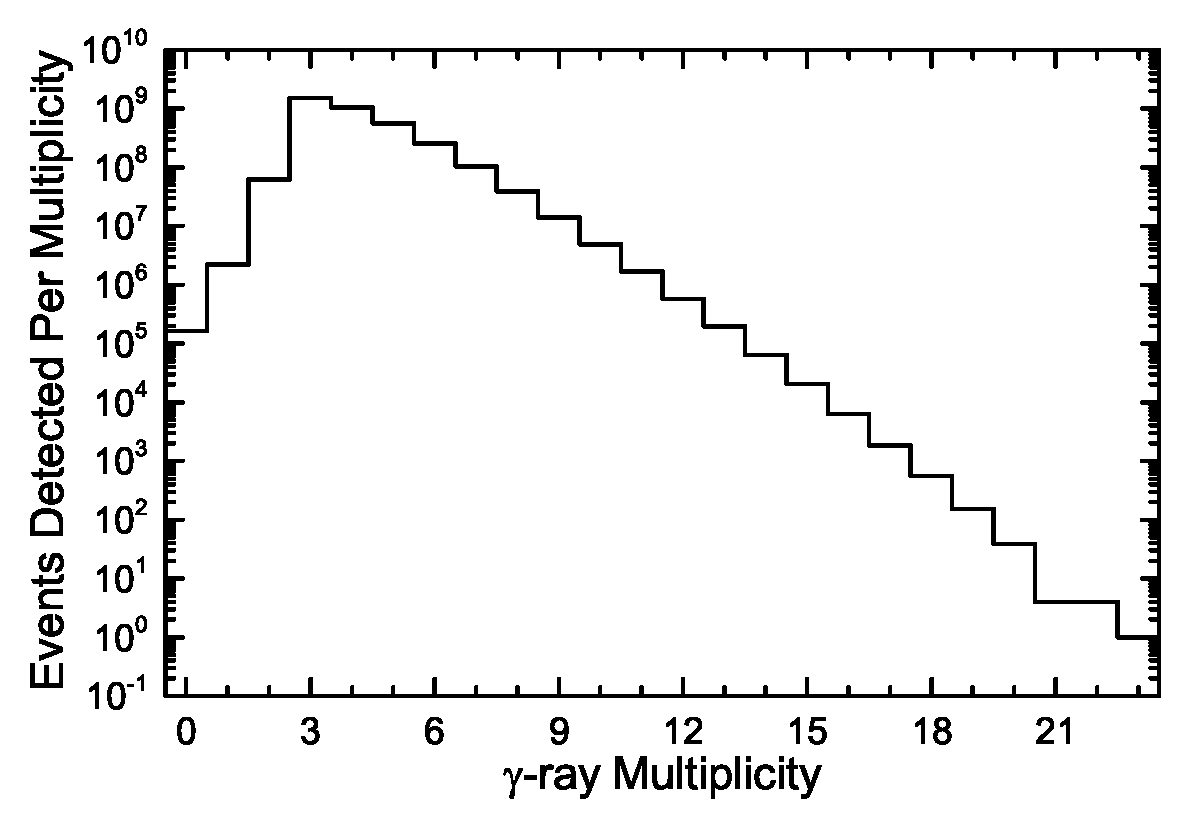
\includegraphics[height=0.25\textheight]{./img/c3/gs_event_plot.eps}}
 	\caption{Histogram of the number of events in each multiplicity for the experiment at Gammasphere.}
 	\label{fig:chp3-gs_event_pattern}
 \end{figure}
 
 In the experiment utilizing INGA $\sim{}550$Gb of data spread across $\sim800$ files were collected. As INGA was run in a triggerless mode each module of electronics output timestamped events in each detector to a file. Afterwards the data are merged into an order according to their timestamp, yielding $\sim{}503$Gb spread across $185$ files. Construction of events then proceeds by setting a coincidence time window and ``scanning'' the window across the merged events looking for sets of events whose timestamps all fall within that window. This process yielded $3.52\times{}10^9$ two- and higher-fold events. This data was used for the extraction of polarizations using the scattering asymmetry at $90^{\circ{}}$. This, coupled with requiring that the energy be seen in two and \emph{only} two of the crystals of a $90^{\circ{}}$ detector, reduced the number of eligible two- and higher-fold events to $3.47\times{}10^8$.
 
\subsection{Calibration}
\label{ssec:exp-pr-data-proc-cal}
Prior to working with the actual data in an experiment it is necessary to perform energy and efficiency calibration of the detectors. For \gr{} detection experiments of this kind calibration involves placing a radioactive source with known lines in the same position that the beam would strike the target. If absolute efficiency is desired as opposed to relative efficiency the activity of the source must be known as well so that one know exactly how many gamma's passed through one's detector. In this case however, only relative efficiency was necessary so this information was neglected.

At Gammasphere this was accomplished by placing a $^{152}$Eu source into the center of the array and changing the multiplicity threshold of the trigger system to one.
\subsection{Background Subtraction}
\label{ssec:exp-pr-data-proc-bg-sub}
\subsubsection{Symmetric Gates}
\label{sssec:exp-pr-data-proc-bg-sub-sym}
\subsubsection{Asymmetric Gates}
\label{sssec:exp-pr-data-proc-bg-sub-asym}

\section{Angular Distributions, Correlations, and Polarization}
\label{sec:exp-pr-data-ang}
\subsection{Angular Distributions}
\label{ssec:exp-pr-data-ang-dist}
Testing 1
\subsection{Angular Correlations}
\label{ssec:exp-pr-data-ang-cor}
\begin{figure}[h!]
	\centerline{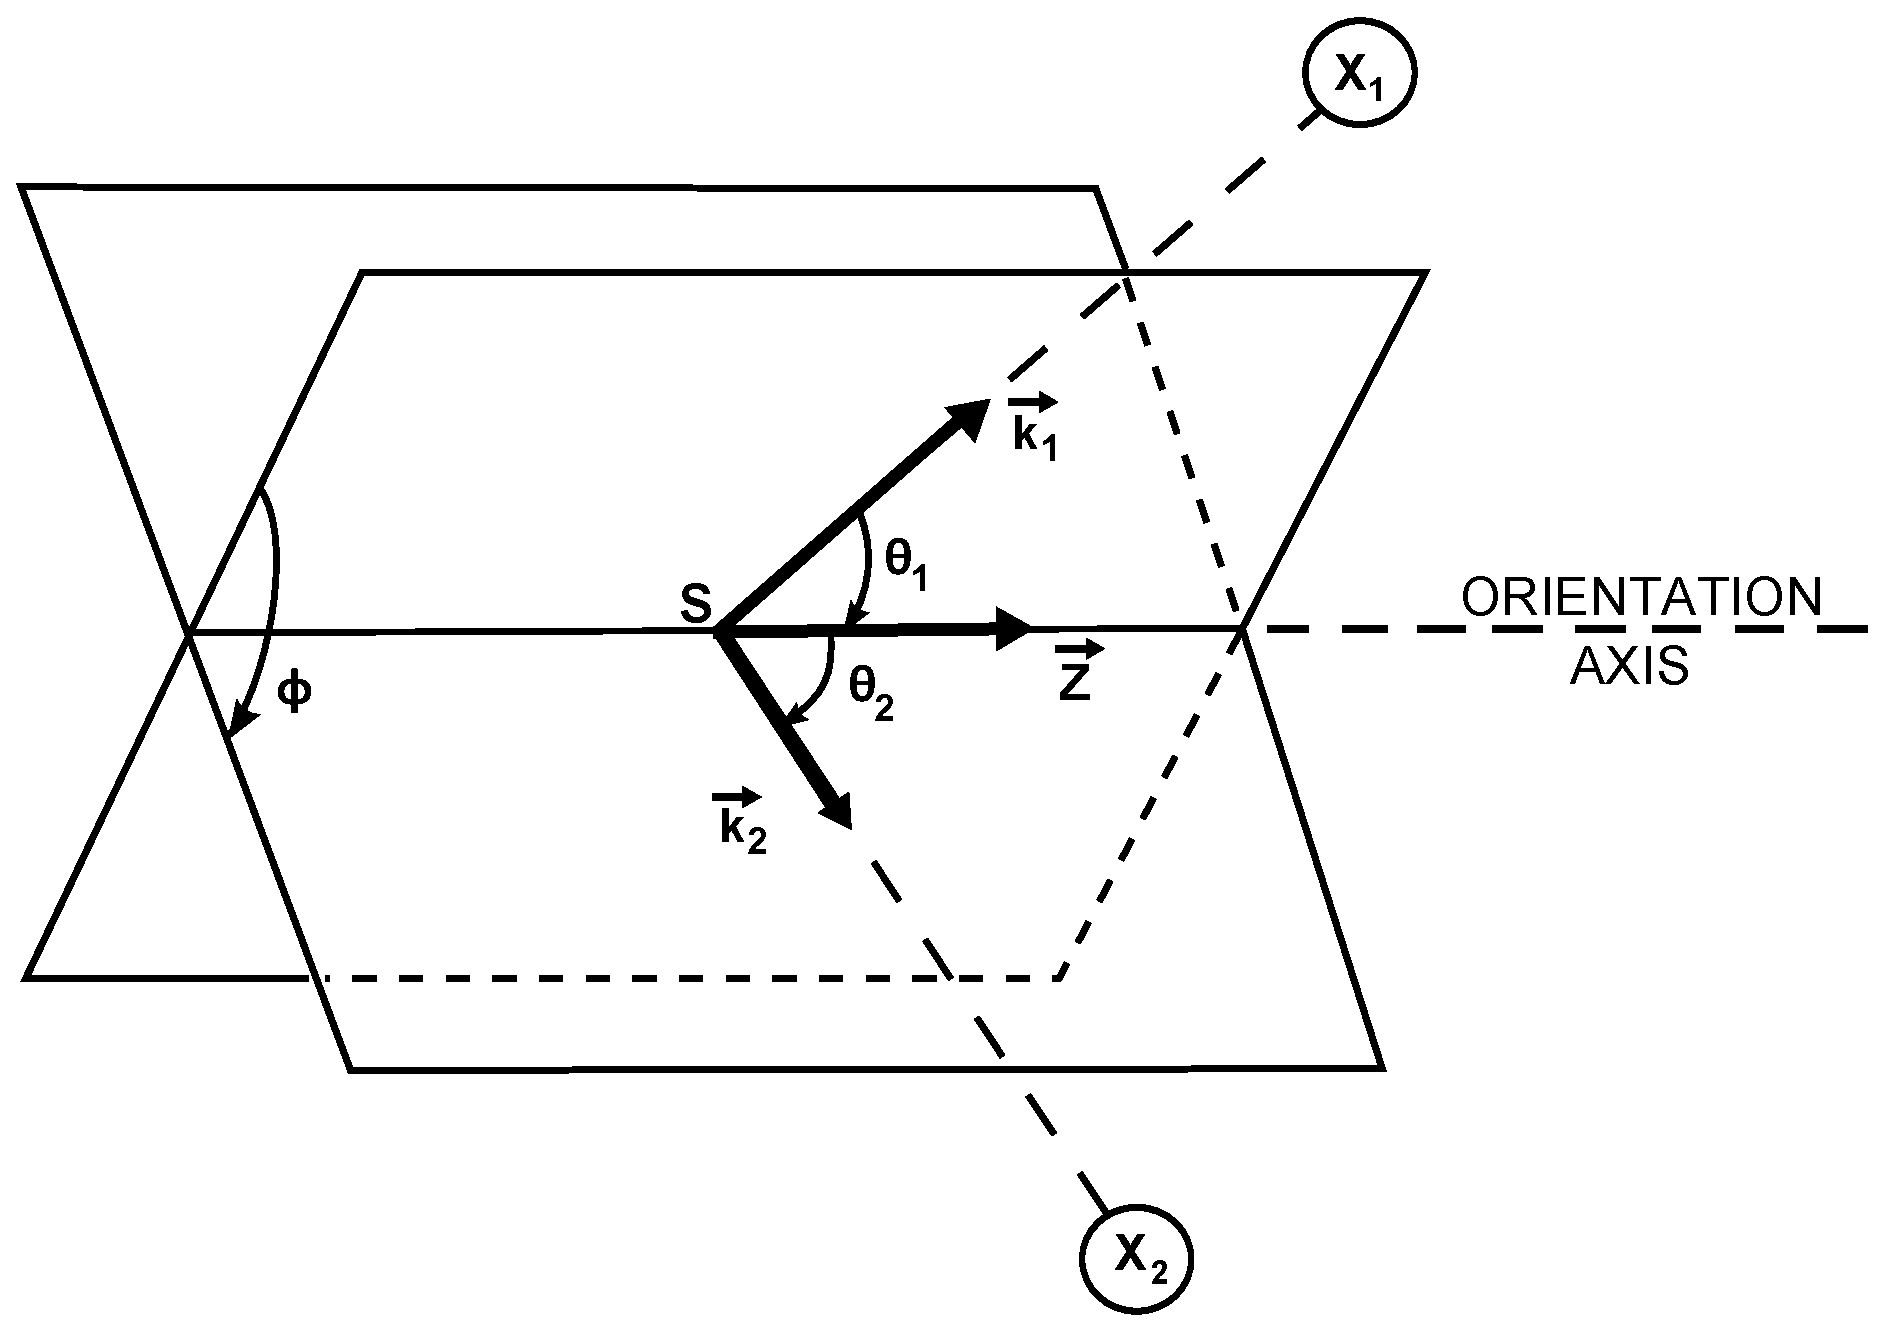
\includegraphics[height=0.35\textheight]{./img/c3/dco_setup.eps}}
	\caption{Diagram of the angles in a directional correlation of two successive radiations X$_{1}$ and X$_{2}$ emitted from an axial symmetric oriented source S.}
	\label{fig:chp3-DCO-Angles}
\end{figure}
\subsubsection{Directional Correlation of Gamma-rays from Oriented Nuclei DCO Ratios}
\label{sssec:exp-pr-data-ang-cor-dco}
Testing 3
\subsection{Polarization}
\label{ssec:exp-pr-data-ang-pol}
Testing 4


%
% Chapter 4 - Transverse wobbling in 135Pr
%
%
%  Chapter:  4 - Transverse Wobbling in 135Pr
%  Modified: 2/16/2015
%  Author:   James Till Matta
%
%%%%%%%%%%%%%%%%%%%%%%%%%%%%%%%%%%%%%%%%%%%%%%%%%%%%%%%%%%

\chapter{TRANSVERSE WOBBLING IN $^{135}$Pr}
\label{chp:trw}
%As stated in chapter \ref{chp:intro} wobbling is the longest anticipated fingerprint of triaxiality. Bohr and Mottelson predicted its existence in 1969 in the first edition of the second volume of their book nuclear structure\cite{bohrMottelson2}. Despite this longstanding prediction of its existence, the first discovery of wobbling was in 2001 by \O{}deg\aa{}rd \emph{et al.} \cite{wobblingIn163Lu}. Prior to this work wobbling had only been seen in five nuclei confined to the $A\sim{}170$ region, $^{161,163,165,167}$Lu \cite{wobblingIn163Lu,wobblingIn161Lu,wobblingIn165Lu,wobblingIn167Lu} and $^{167}$Ta \cite{wobblingIn167Ta}.

%Wobbling is the harmonic vibration of a nucleus's principal axis about its angular momentum vector. In the body fixed or intrinsic frame, wobbling is the harmonic vibration of the nucleus's angular momentum vector about one of its principal axes. In the simple wobbling mode, the principal axis used as a reference is the intermediate axis. This intermediate axis has the largest moment of inertia (MOI) and absent anything else is the preferred axis of rotation. In the transverse wobbling the reference principal axis is either the short or long axes as they are the axes that a quasiparticle with primarily particle nature or hole nature will couple to respectively. This coupling forces the rotation and wobbling motion to occur about these axes, eventually though the motion will become unstable and the wobbling will collapse as the rotation realigns itself to a new vector in the plane between the intermediate axis and the original axis of rotation. The final mode, longitudinal wobbling occurs when the Coriolis force aligns the quasiparticle to the intermediate axis. As in the simple wobbling case the rotation and wobbling occurs about the intermediate axis.
Understanding of the wobbling mode in nuclei has evolved quickly over the last 15 years. Bohr and Mottelson first showed that a rotating nucleus with stable triaxially deformed could have its rotational angular momentum precess and nutate about the principal axis of a nucleus (in analogy to the classical asymmetric top) \cite{bohrMottelson2} quite some time ago. H. Schnack-Petersen \emph{et al.} suggested in 1995 that bands in $^{163,165}$Lu which are based on the $\pi{}(i_{13/2})$ configuration, occupied a triaxial superdeformed (TSD) minimum of the total routhian surface \cite{tsdLutetium}. Following this there was rash of wobbling discoveries in $^{161,163,165,167}$Lu from 2001 to 2005 \cite{wobblingIn163Lu,wobblingIn163LuTwoPhonon,wobblingIn165Lu,wobblingIn167Lu,wobblingIn161Lu}. Further searches conducted in the region on $^{171}$Ta \cite{wobbSearch171Ta}, $^{169}$Ta \cite{wobbSearch169Ta}, $^{163}$Tm \cite{wobbSearch163Tm}, $^{171,172}$Hf \cite{wobbSearch1712Hf}, and ${160,161}$Tm \cite{wobbSearch1601Tm} yielded no further wobbling bands. This left an open problem as to why wobbling was only appearing in the Lu isotopes.

A possible solution to this problem was offered up in the TAC calculations by S. Frauendorf presented in Ref. \cite{wobbSearch163Tm}. The calculations suggest that the Lu TSD minima have a low density of states, low enough that the relatively high excitation energy wobbling mode can be observed. Contrariwise, the TSD minima of other nuclei in the region had a high density of states which could produce many different TSD bands with alternate configurations at similar energies. Thus, it is not that wobbling is absent in nuclei that are not Lu isotopes, but instead, that outside of the Lu isoptopes there was a competition between wobbling and particle hole excitations that favored the latter. This result motivated a search of $^{167}$Ta for wobbling which, in 2009, yielded the first wobbling band outside the Lu isotopes.


\section{Previous Cases of Wobbling}
\label{sec:trw-prev}
One phonon wobbling was first observed in 2001 in the nucleus $^{163}$Lu by S.W. \O{}deg\aa{}rd \emph{et al.} \cite{wobblingIn163Lu}. In 2002 two phonon wobbling was observed in the same nucleus by D.R. Jensen \emph{et al.} \cite{wobblingIn163LuTwoPhonon} (partial level scheme pictured in the left panel of Fig. \ref{fig:chp4-first-wobb}). In 2003 one and two phonon wobbling was discovered in $^{165}$Lu by G. Sch\"onwa\ss{}er \emph{et al.} \cite{wobblingIn165Lu} (partial level scheme pictured in the right panel of Fig. \ref{fig:chp4-first-wobb}). Later that same year came the discovery of one phonon wobbling in $^{167}$Lu by H. Amro \emph{et al.} \cite{wobblingIn167Lu} (partial level scheme pictured in the left panel of Fig. \ref{fig:chp4-second-wobb}). 2005 was the year of the discovery of one phonon wobbling  $^{161}$Lu by P. Bringel \emph{et al.} \cite{wobblingIn161Lu} (partial level scheme pictured in the right panel of Fig. \ref{fig:chp4-second-wobb}). The last of the wobblers known prior to this work, $^{167}$Ta, was discovered in 2009 by D.J. Hartley \emph{et al.} \cite{wobblingIn167Ta} (partial level scheme pictured in Fig. \ref{fig:chp4-last-wobb}). 

\begin{figure}[ht!]
\centerline{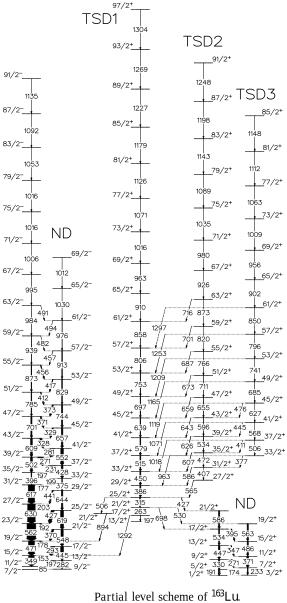
\includegraphics[width=0.4\textwidth]{./img/c4/163Lu_scheme.png}\hspace{0.1\textwidth}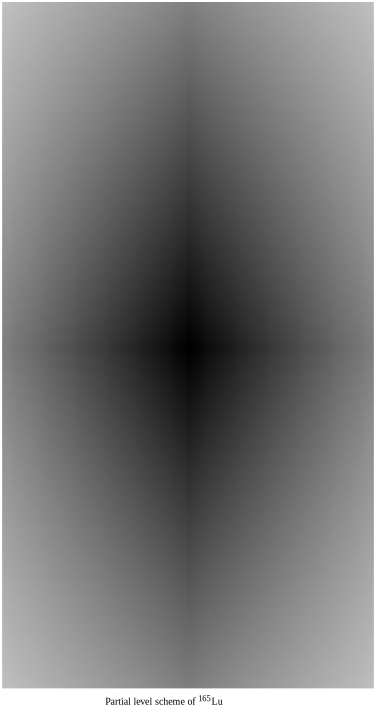
\includegraphics[width=0.4\textwidth]{./img/c4/165Lu_scheme.png}}
	\caption{Partial level schemes of $^{163}$Lu (left) and $^{165}$Lu (right). Figures adapted from Ref. \cite{wobblingIn163LuTwoPhonon} and Ref. \cite{wobblingIn165Lu} respectively. In $^{163}$Lu the $n_w=0,1,2$ bands are labeled TSD1, TSD2, and TSD3 respectively. In $^{165}$Lu the $n_w=0,1,2$ bands are labeled TSD1, TSD2, and TSD3 respectively.\label{fig:chp4-first-wobb}}
\end{figure}

\begin{figure}[ht!]
\centerline{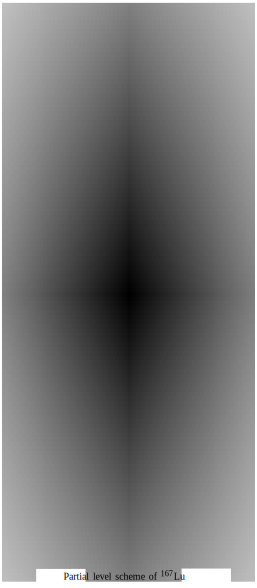
\includegraphics[width=0.4\textwidth]{./img/c4/167Lu_scheme.png}\hspace{0.1\textwidth}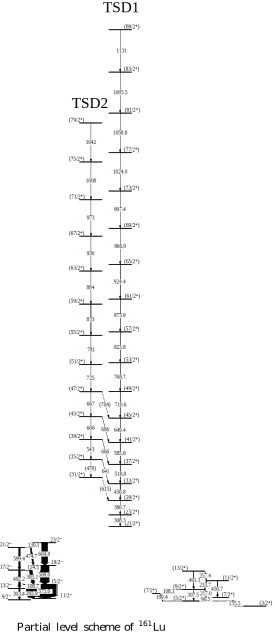
\includegraphics[width=0.4\textwidth]{./img/c4/161Lu_scheme.png}}
	\caption{Partial level schemes of $^{167}$Lu (left) and $^{161}$Lu (right). Figures adapted from Ref. \cite{wobblingIn167Lu} and Ref. \cite{wobblingIn161Lu} respectively. In $^{167}$Lu the $n_w=0,1$ bands are labeled TSD1 and TSD2 respectively. In $^{161}$Lu the $n_w=0,1$ bands are labeled TSD1 and TSD2 respectively.\label{fig:chp4-second-wobb}}
\end{figure}

\begin{figure}[ht!]
\centerline{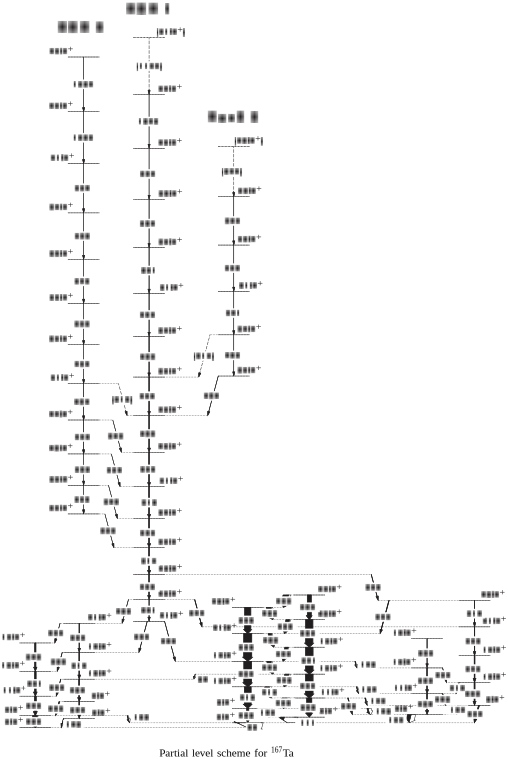
\includegraphics[width=0.6\textwidth]{./img/c4/167Ta_scheme.png}}
	\caption{Partial level scheme of $^{167}$Ta. Figure adapted from Ref. \cite{wobblingIn167Ta}. The $n_w=0,1$ bands are labeled TSD1 and TSD2 respectively.\label{fig:chp4-last-wobb}}
\end{figure}

Following the discovery of the first wobbling structure, calculations using the QTR model were used to describe the wobbling mode \cite{oldQTRWobblingTheory1,oldQTRWobblingTheory2,oldQTRWobblingTheory3,oldQTRWobblingTheory4}. Later, microscopic random phase approximation (RPA) calculations \cite{wobblingRPAMatsuzaki,wobblingRPAMatsuzaki2,wobblingRPAOi,wobblingRPAShimizu,wobblingRPAshoji} were used as well. Both theories do well in reproducing the large $B(E2)_{out}/B(E2)_{in}$ interband to intraband ratios seen in experiment. However, the QTR model, using the assumptions that the odd quasiparticle aligns with the intermediate axis \cite{oldQTRWobblingTheory1,oldQTRWobblingTheory2,oldQTRWobblingTheory3,oldQTRWobblingTheory4}, failing to reproduce the experimentally observed decrease in the wobbling energy (see Fig. \ref{fig:chp4-old-wobb-freq}) which is defined by:
\begin{equation}
\label{eqn:chp4-wobb-freq}
\Delta{}E=\hbar\omega_w(I)=E(I,n_w=1)-(E(I-1,n=0)+E(I+1,n_w=0))/2
\end{equation}
In constrast the microscopic RPA calculations were able to reproduce the observed decrease in wobbling energy.
\begin{figure}[ht!]
\centerline{\includegraphics[height=0.25\textheight]{./img/c4/163Lu_plot.eps}\hspace{0.1\textwidth}\includegraphics[height=0.25\textheight]{./img/c4/165Lu_plot.eps}}
\centerline{\includegraphics[height=0.25\textheight]{./img/c4/167Lu_plot.eps}\hspace{0.1\textwidth}\includegraphics[height=0.25\textheight]{./img/c4/161Lu_plot.eps}}
\centerline{\includegraphics[height=0.25\textheight]{./img/c4/167Ta_plot.eps}}
	\caption{Wobbling frequencies of the $A\sim{}170$ wobblers. Top Left: $^{163}$Lu. Top Right: $^{165}$Lu. Middle Left: $^{167}$Lu. Middle Right: $^{161}$Lu. Bottom: $^{167}$Ta.\label{fig:chp4-old-wobb-freq}}
\end{figure}

To correct the deficiency in the QTR calculations of wobbling, S. Fraendorf and F. D\"onau introduced the concept of transverse and longitudinal wobbling \cite{frauendorfTransverseWobbling}. In this new scheme Refs. \cite{oldQTRWobblingTheory1,oldQTRWobblingTheory2,oldQTRWobblingTheory3,oldQTRWobblingTheory4} were describing longitudinal wobbling which is indeed expected to have an increasing wobbling frequency. A semi-classical analysis of transverse wobbling, which has the quasiparticle couple to an axis perpendicular to the intermediate axis, shows that the modified mode exhibits a decreasing wobbling frequency as has been seen in experimental observations of wobbling while reproducing the interband to intraband $B(E2)$ ratios.


\section{Triaxiality in the A$\sim{}130$ Region}
\label{sec:trw-triax}
As mentioned earlier in this dissertation, the wobbling mode is signature of stable triaxial deformation. That is to say that without stable triaxial shapes the there will be no wobbling excitations. As triaxiality has been a subject of general interest to the nuclear structure community for many years this makes observation of the wobbling mode important as constitutes irrefutable evidence of triaxiality. 

Another important signature of triaxial shape is nuclear chirality. Here a particle-like quasiparticle couples to the short axis, a hole like quasi-particle couples to the long axis, and the triaxial rotor core rotates about the intermediate axis. In this configuration the total angular momentum points away from any of the principal planes of the nucleus and its the three components form a screw with respect to it \cite{frauendorfChirality}. When this configuration is present, the time-reversal symmetry of the wave functions is broken and two nearly degenerate $\Delta{}I=1$ bands with similar electromagnetic properties emerge. Without triaxiality this situation cannot arise and therefore observation of nuclear chirality again gives proof of a stable triaxial shape.

Predictions made by M\"oller \emph{et al.} in Ref. \cite{groundStateTriax} show that the region around $Z=60$ and $N=76$ has triaxial shapes at low to moderate spin. This prevalence of triaxial shapes in this region is confirmed by the numerous observations of chirality \cite{chiralityIn134Pr,chiralityA130Region,chiralityUpperA130Region,chiralityA130Region2,chirality136Pm,chiralityMore135Nd,chiralityIn135Nd,chiralityMulti133Cs}. Additionally, a more exotic and stable chirality was identified in \cite{chiralityMore135Nd,chiralityIn135Nd} and confirmed via lifetime measurement to extract the $B(M1)$ and $B(E2)$ values of the partner bands to ensure that they are the same \cite{chiralityIn135Nd}. In fact, in this observation a transition from more usual chiral vibration (where the angular momentum vector oscillates in a plane perpendicular to the axes the quasiparticles are coupled to) to static chirality where this oscillation slows to nearly stationary resulting in the bands becoming quite close to degenerate.

\section{Level Scheme of $^{135}$Pr}
\label{sec:trw-lvl-scheme}
Data from the Gammasphere experiment, described in \ref{sec:exp-pr-details}, were sorted into symmetrized cubes (E$_{\gamma{}}$-E$_{\gamma{}}$-E$_{\gamma{}}$) and hypercubes (E$_{\gamma{}}$-E$_{\gamma{}}$-E$_{\gamma{}}$-E$_{\gamma{}}$) using the RADWARE suite of codes \cite{radware}. Background subtracted gated spectra were obtained using the RADWARE suite coupled with the background subtraction algorithm of Ref. \cite{symBGSub}. The smooth backgrounds used for this algorithm are shown in Fig. \ref{fig:chp4-bg-specs}. Coincidence relations from this data were used to reconstruct the level scheme.
\begin{figure}[bh!]
\centerline{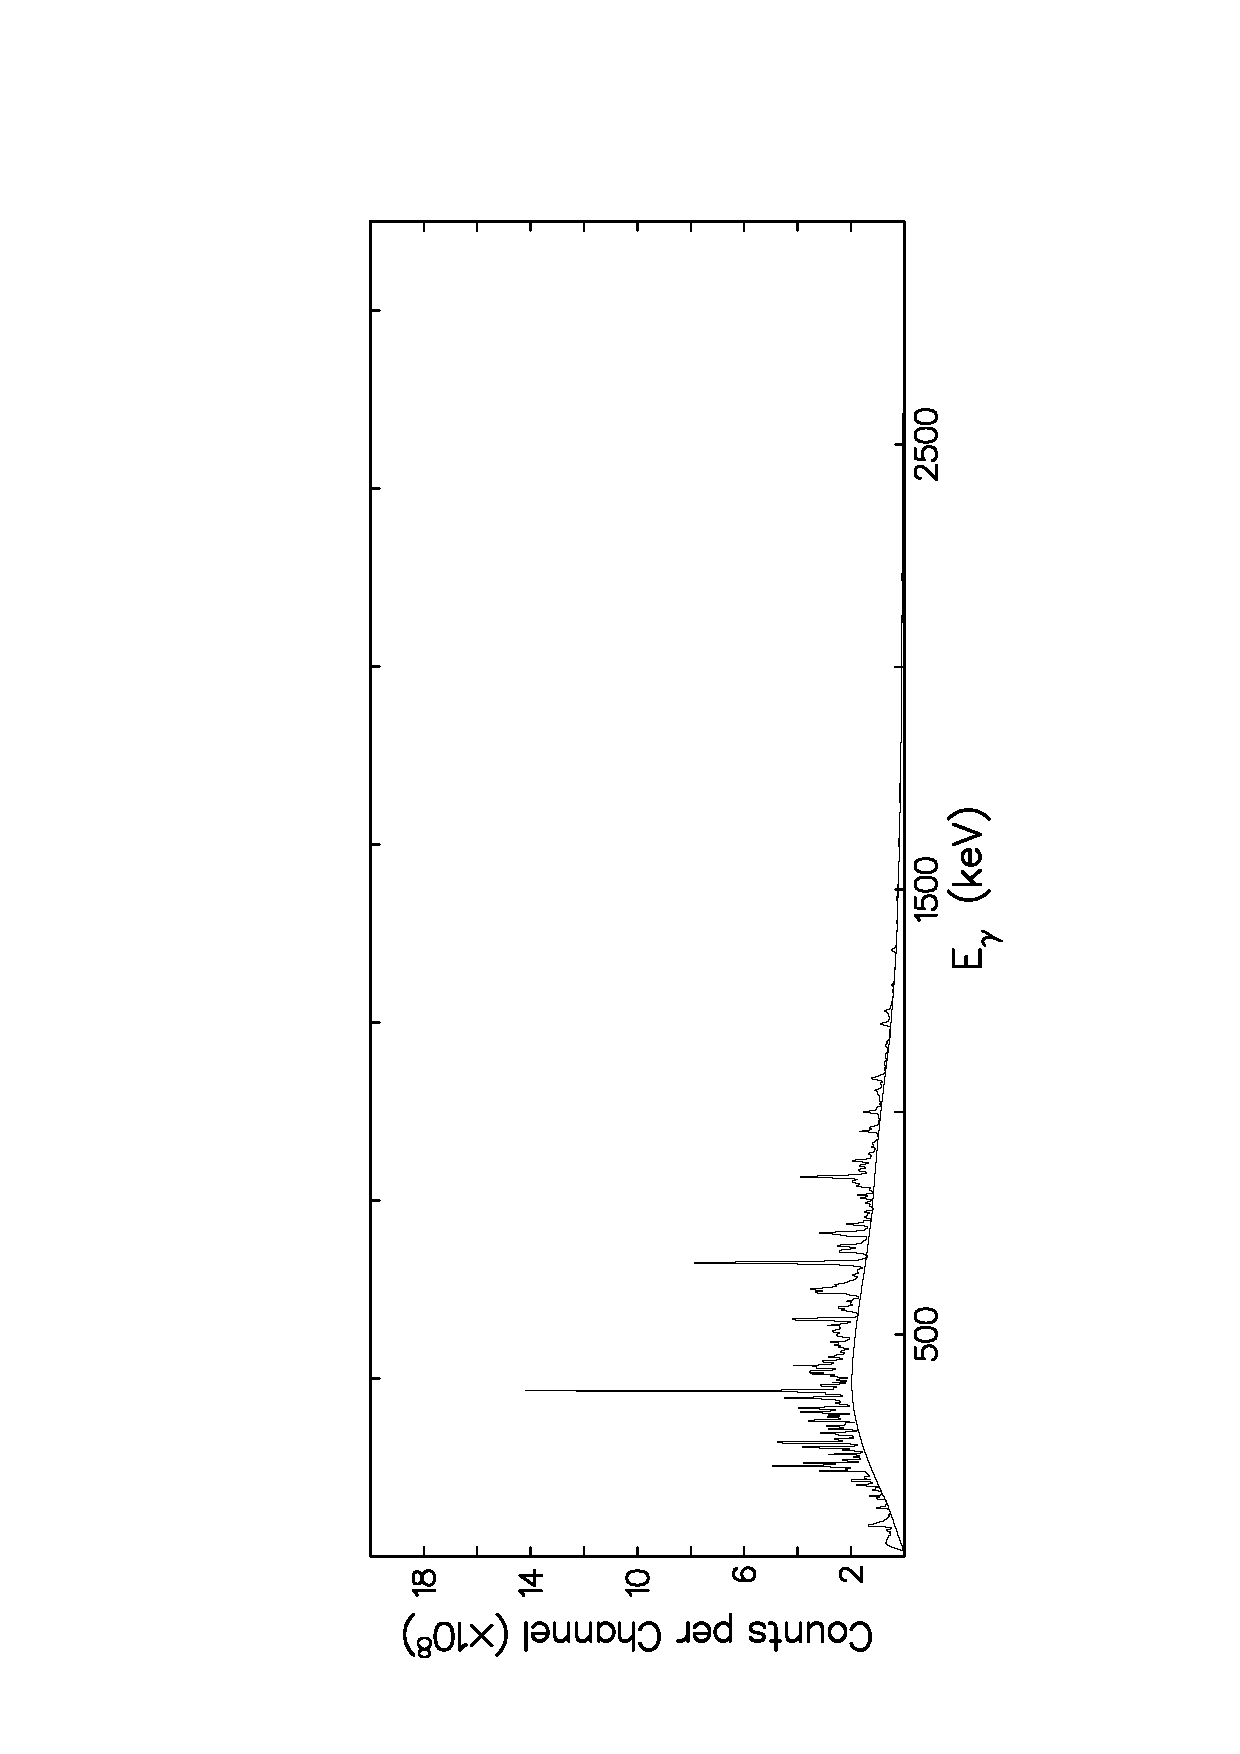
\includegraphics[width=0.45\textwidth]{./img/c4/trips_bg.pdf}\hspace{0.09\textwidth{}}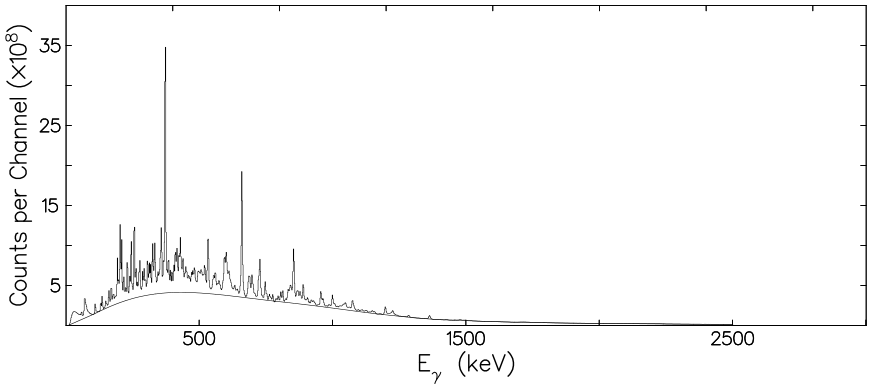
\includegraphics[width=0.45\textwidth]{./img/c4/quads_bg.pdf}}
	\caption{Left: Background spectrum for the symmetrized cube. Right: Background spectrum for the symmetrized hypercube. \label{fig:chp4-bg-specs}}
\end{figure}

\begin{figure}[ht!]
\centerline{\includegraphics[width=\textwidth]{./img/c4/old_scheme.png}}
	\caption{Previous level scheme for \pr{}, from Ref. \cite{semkow135Pr}. \label{fig:chp4-semkow-lvl-schm}}
\end{figure}

\begin{figure}[hb!]
\centerline{\includegraphics[height=0.4\textheight]{./img/c4/old_scheme_bands.png}\hspace{0.1\textwidth}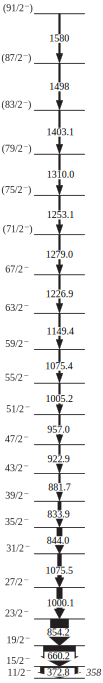
\includegraphics[height=0.4\textheight]{./img/c4/high_spin_yrast.pdf}}
	\caption{Left: Negative parity rotational band structure proposed for \pr{} in Ref. \cite{semkow135Pr}. Right: Yrast band presented in Ref. \cite{ePaul135Pr}. \label{fig:chp4-prev-bands}}
\end{figure}

Previously, T.M. Semkow \emph{et al.} performed a spectroscopic study of \pr{} in  Ref. \cite{semkow135Pr} using a $\gamma$-ray detector array consisting of four HPGe detectors with NaI escape suppression, two unsuppressed HPGe detectors, and eleven NaI counters (to provide $\gamma$-ray multiplicity selection). In this experiment $1.66\times{}10^8$ $\gamma{}$-$\gamma{}$ events were collected. Using this data, the level scheme in Fig. \ref{fig:chp4-semkow-lvl-schm}, showing both positive and negative parity levels, was developed. As the positive parity portion of the level scheme is of little interest to the wobbling excitation in \pr{}, it is neglected for the rest of this work. Later in Ref. \cite{semkow135Pr}, rotational band structures for the positive and negative parity parts of the level scheme were proposed, the left panel Fig. \ref{fig:chp4-prev-bands} contains the proposed negative parity rotational band structure. Additional work, extending the yrast band to $\sfrac{91}{2}$, was done by E.S. Paul \emph{et al.} in Ref. \cite{ePaul135Pr}. The data for the work in Ref. \cite{ePaul135Pr} was a byproduct of a high statistics measurement of $^{134}$Pr done at Gammasphere. The right panel of Fig. \ref{fig:chp4-prev-bands} contains the proposed yrast structure.


\begin{landscape}
\begin{figure}[h!]
\centerline{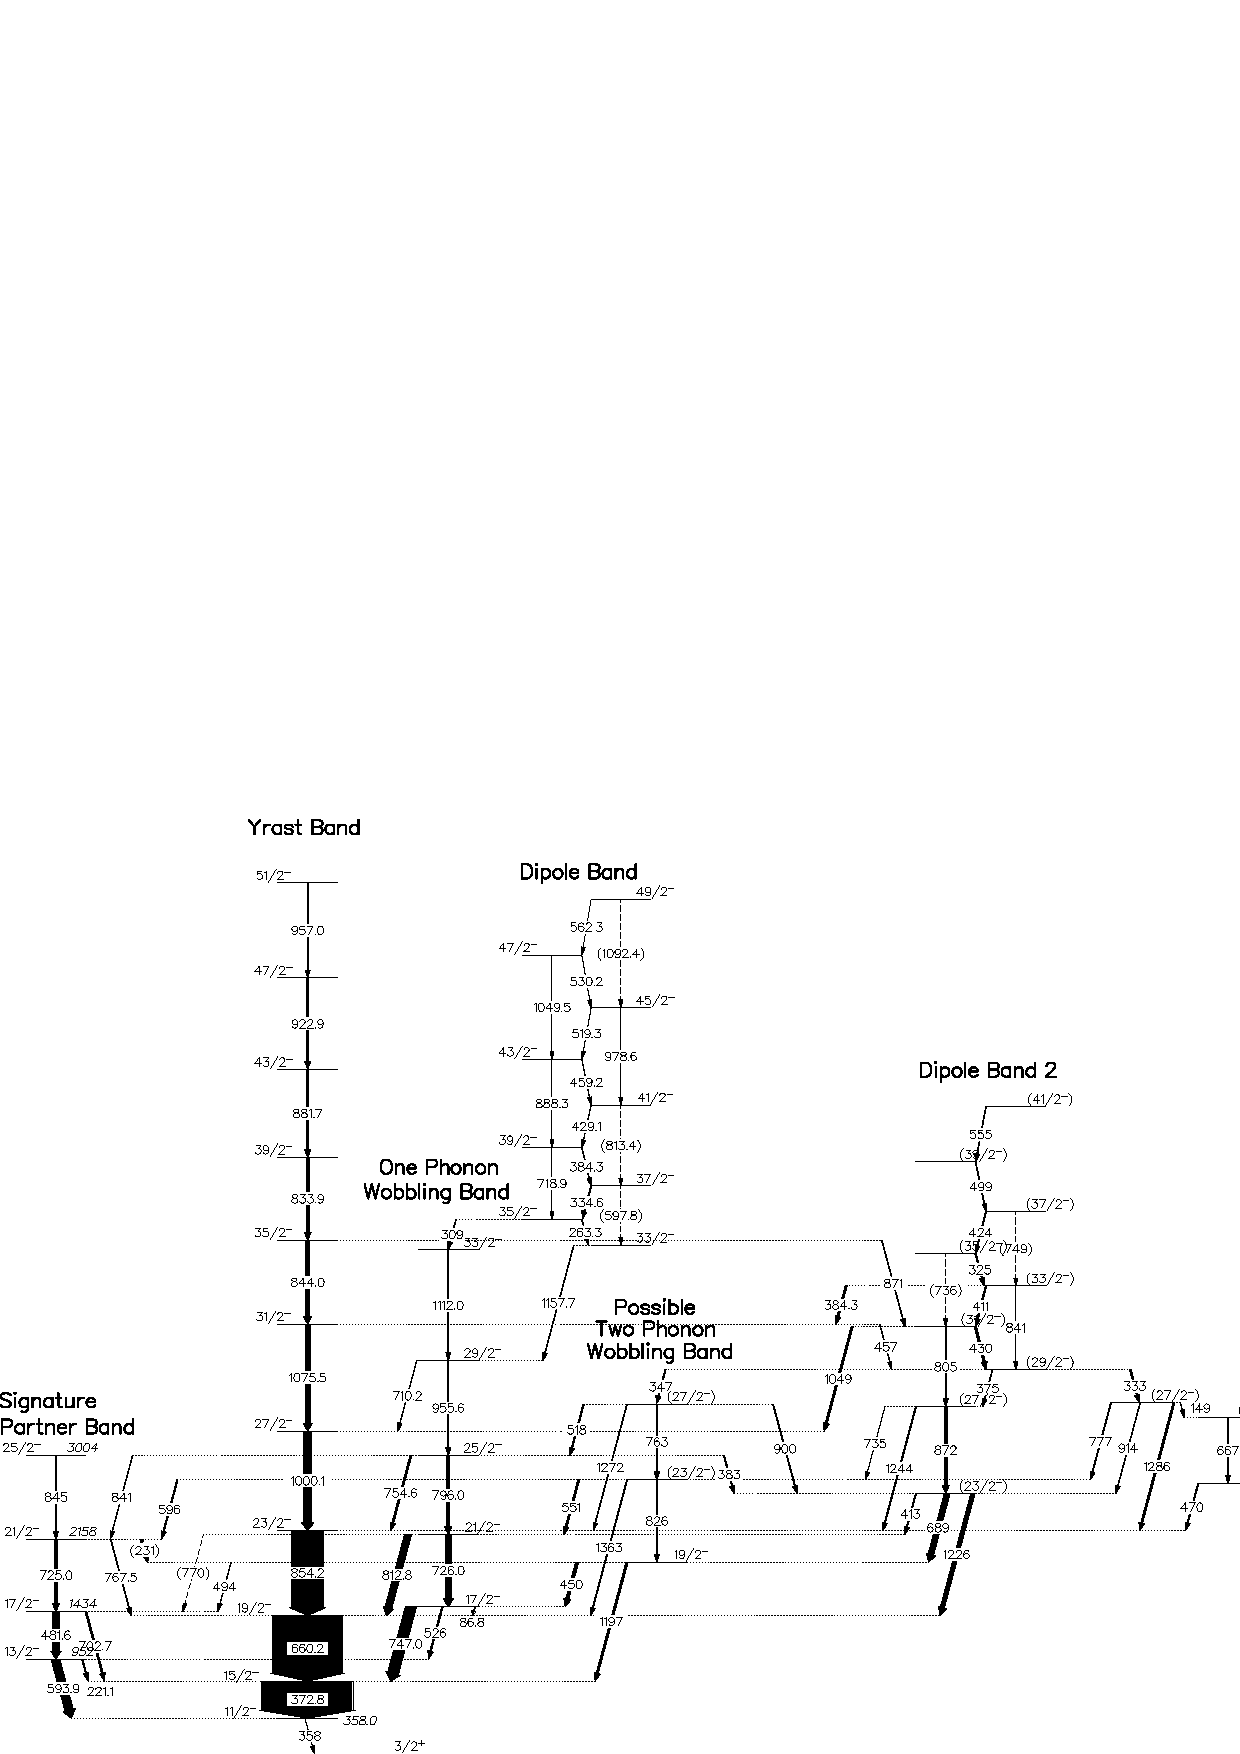
\includegraphics[height=0.9\textheight]{./img/c4/135Pr_Np_for_diss.pdf}}
	\caption{Negative parity level scheme developed for \pr{}. \label{fig:chp4-neg-par-lvl-schm}}
\end{figure}
\end{landscape}

The negative parity level scheme constructed from the Gammasphere data in this work is presented in Fig. \ref{fig:chp4-neg-par-lvl-schm}. Tables of level and transition information can be found in Appendix \ref{app:neg-par-info}. As the beam and target pair of the reaction were tuned to preferentially excite non-yrast states the yrast band was only measured to spin $\sfrac{51}{2}$. The finding of this measurement were in agreement with Ref. \cite{ePaul135Pr}. However, the band structure proposed in Ref. \cite{semkow135Pr} was in disagreement with the results found in this work. Notably, the signature partner transitions above the $\sfrac{25}{2}$ level were found to instead belong to the $n_w=1$ wobbling band. It seems that the previous work here was unable to resolve the difference between the last $845$ keV transition of the signature partner band and the $841$ keV transition linking the $n_w=1$ wobbling band to the signature partner band. Evidence for the this is given in Figs. \ref{fig:chp4-spec-dbl-gates} and \ref{fig:chp4-spec-triple-gate}. Fig. \ref{fig:chp4-spec-dbl-gates} shows the sum of the spectra resulting from every possible double gate on the dipole band. This spectrum shows the dominance of decay through the wobbling band as opposed to the signature partner band. Fig. \ref{fig:chp4-spec-triple-gate} shows a triple gate placed on the $n_w=1$ band and the dipole band immediately above the weak linking transition from the wobbling band to the signature partner band. Here the difference in the $841$ keV transition's strength and the strength of the $796$ keV transition plainly visible. This disparity in strength further highlights that the primary decay path from the $\sfrac{25}{2}$ is through the $796$ keV transition, in keeping with it being an intraband transition.

\begin{figure}[h!]
\centerline{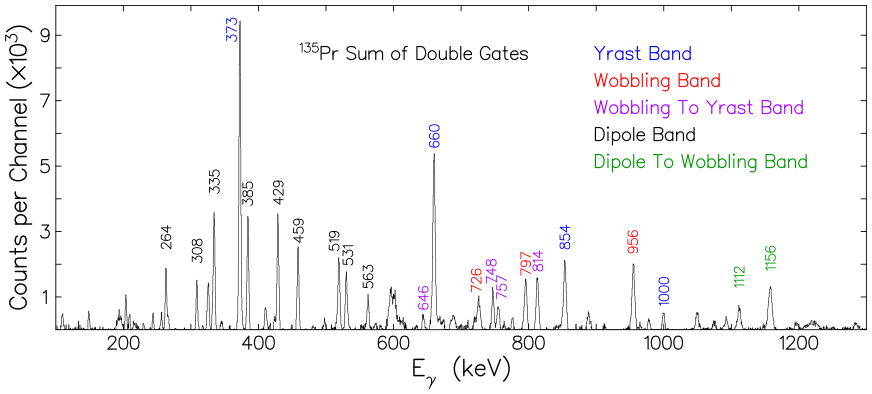
\includegraphics[width=\textwidth]{./img/c4/sum_of_dbl_gate_ev.pdf}}
	\caption{Sum of all possible double gates on M1 transitions in the dipole band. The labeling of the transitions is color coded according to the band the transition belongs to. \label{fig:chp4-spec-dbl-gates}}
\end{figure}
\begin{figure}[h!]
\centerline{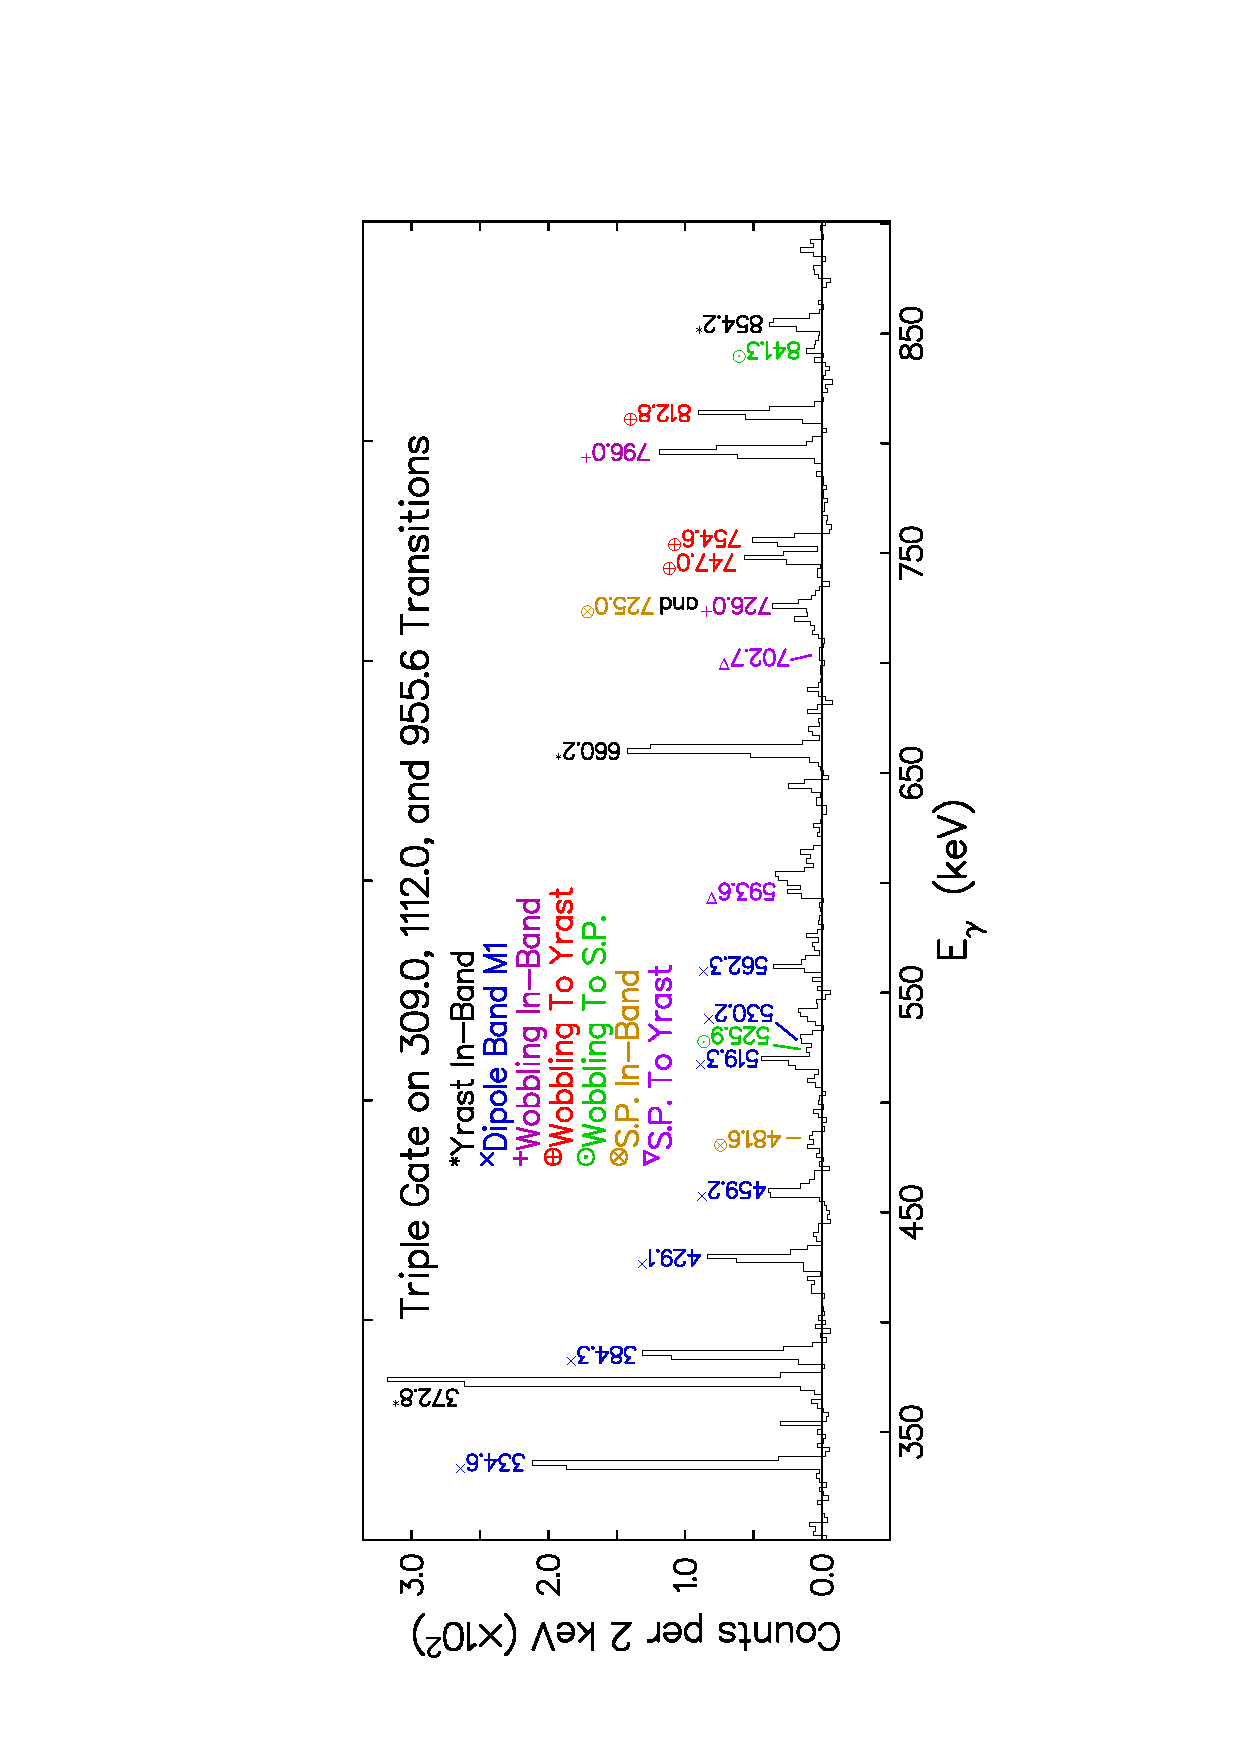
\includegraphics[width=\textwidth]{./img/c4/trip_gate_ev.pdf}}
	\caption{Sum of triple gate on the specified transitions. The labeling of the transitions is color coded according to the band the transition belongs to. \label{fig:chp4-spec-triple-gate}}
\end{figure}

Spins were assigned through the following techniques: angular distributions (method discussed in section \ref{sssec:exp-pr-data-ang-cor-dco}), DCO-like ratios (method discussed in section \ref{sssec:exp-pr-data-ang-cor-dco}) and arguments from the deexcitation of the level to multiple levels. Assignments using the first two methods are discussed in section \ref{ssec:trw-lvl-angles}; however, as the third method is relies purely on coincidence data and previously known components of the level scheme it will be addressed here.

The dipole and quadrupole transitions of Dipole Band 1 and Dipole Band 2 were assigned based on their placement. As each dipole transition (strong low energy transitions) had a cross-over transition the following reasoning was used. A cross-over transition must have a low-order multipolarity (L) equal to the sum of the low-order multipolarities of the two transitions it crosses. Therefore, a crossover of $E2$ nature is only possible if the two crossed transitions are both dipole. If one or both of the crossed transitions is of higher order then the crossing transition must be of higher order as well. Given the very low probability (slow) nature of most transitions with $L>2$ observation of the cross-over shows that the cross-over must be $E2$ and the crossed transitions $M1$. Though the top of Dipole Band 2 had cross-over transitions that were too weak to measure the observation of lower cross-over transitions and their rapidly fading strength gave confidence in the band continuing to be composed of $M1$ transitions.

The spin of dipole band 2 was fixed relative the yrast band using the four interband transitions that link the states around $\sfrac{31}{2}$ of the two bands. The pattern of linking that occurred is typical of levels that happened to mix because they were very close in energy and had the same spin and parity. Additionally, if the two apparently overlapped states were separated by one unit of angular momentum then either the $871$ keV transition or the $1049$ keV transition would have $L=3$, rendering it highly improbable. Unfortunately, this argument does not cover the $\sfrac{23}{2}$ state of dipole band 2. This state's spin was fixed by the following arguments: if the state were instead $\sfrac{21}{2}$ then the $872$ keV transition would be a highly improbable $L=3$, while if it were $\sfrac{25}{2}$ then the $689$ keV and $1226$ keV transitions would both be $L=3$, again, an improbability. The spin of the signature partner band $\sfrac{21}{2}$ level is fixed as follows. If the level were instead $\sfrac{19}{2}$, the $841$ keV transition into it would be $L=3$ in nature. Alternatively, if the level were$\sfrac{23}{2}$ then the $725$ keV transition out of it would be $L=3$. Finally, the spin of the $\sfrac{27}{2}$ was fixed as follows: If the level were $\sfrac{29}{2}$ then $1272$ keV transition would be $L=3$. Supporting the impossibility of the level being $\sfrac{25}{2}$ are these facts the $518$ keV transition would be $L=0$ which is less probable, additionally, the $1272$ keV transition would be $L=1$. If the $1272$ keV transition were $L=1$ then it could be either $M1$ or $E1$. The $M1$ possibility is highly unlikely due to rarity of $M1$ transitions with such high energy, The $E1$ possibility is countered by the large number of transitions linking the level to other negative parity levels. It would be highly improbable for the level to be of different parity from the majority of levels it connects to.

\subsection{Angular Distributions and DCO-like Ratios}
\label{ssec:trw-lvl-angles}

The first step in determining if a band is an $n_w=x$ wobbling band is to look at transitions from $n_w=x$ to $n_w=(x-1)$. For the case studied in this work, $x=1$. As stated earlier, these transitions must have $\Delta{}I=1, E2$ nature. To determine if this holds true, angular distributions of the transitions must be extracted and fitted.

Angular distributions for the first three transitions from $n_w=1\rightarrow{}n_w=0$ are plotted in the top left, top right, and middle left panels of Fig. \ref{fig:chp4-angular-distributions}. Each panel contains a plot of the extracted data, a plot of the fit to the data, and plots of the distributions for pure transitions of higher and lower order. As can be seen in the figures the angular distributions for the $n_w=1\rightarrow{}n_w=0$ transitions are strongly mixed with the higher order nature. The shows that the transitions are $\Delta{}I=1, L=2$, while it is highly probably that the polarization of the transition is $E$, to \emph{guarantee} that the transition is $E2$ polarization measurements are necessary. The middle right panel of Fig. \ref{fig:chp4-angular-distributions} holds the angular distribution of the first transition from the band identified as a possible $n_w=2$ band to the $n_w=1$ band. As can be seen in the figure, this distribution is also highly mixed. This is a hopeful sign that the band is in fact the $n_w=2$ band. 

To ensure that the signature partner to yrast transitions are of substantially different character, the bottom left panel of Fig. \ref{fig:chp4-angular-distributions} contains the angular distribution of the first signature partner to yrast transition. Examination of this transition shows that it is less than $3\%~E2$, as expected of signature partner to yrast transition. As an additional check on the angular distribution extraction and fitting procedure the
\begin{figure}[t!]
\centerline{\includegraphics[width=0.475\textwidth]{./img/c4/747Dist_Plot.eps}\hspace{0.04\textwidth}\includegraphics[width=0.475\textwidth]{./img/c4/813Dist_Plot.eps}}
\centerline{\includegraphics[width=0.475\textwidth]{./img/c4/755Dist_Plot.eps}\hspace{0.04\textwidth}\includegraphics[width=0.475\textwidth]{./img/c4/450Dist_Plot.eps}}
\centerline{\includegraphics[width=0.475\textwidth]{./img/c4/594Dist_Plot.eps}\hspace{0.04\textwidth}\includegraphics[width=0.475\textwidth]{./img/c4/1075Dist_Plot.eps}}
	\caption{Important angular distributions fitted in this work. Top Left: The first $n_w=1\rightarrow{}n_w=0$ transition ($747.0$ keV). Top Right: The second $n_w=1\rightarrow{}n_w=0$ transition ($812.8$ keV). Mid Left: The third $n_w=1\rightarrow{}n_w=0$ transition ($754.6$ keV). Mid Right: The first possible $n_w=2\rightarrow{}n_w=1$ transition ($450.1$ keV).  Bottom Left: The first signature partner to yrast transition ($593.9$ keV). Bottom Right: The fifth yrast in-band transition ($1075.5$ keV).\label{fig:chp4-angular-distributions}}
\end{figure}
angular distribution of the fifth yrast in-band transition. As it's nature is $\Delta{}I=2, E2$, substantially different from the transitions fitted previously, flaws in the procedure that may be hidden for $\Delta{}I=1$ transitions should be more easily visible. As shown in the bottom right panel of Fig. \ref{fig:chp4-angular-distributions}, this check revealed no issues, as expected the transition was found to be pure $E2$ in nature.
 
Angular distributions provide a highly detailed examination of a transitions multipolarity; however, because any gates to clean the resultant spectra must be placed below the transition of interest, and because the intensity of the transition is distributed across many rings, they can be difficult and time consuming to extract. As mentioned in section \ref{sssec:exp-pr-data-ang-cor-dco} DCO-like ratios are a convenient method for extracting the multi-polarity of the distribution. While it is much harder to get a good limit on the mixing ratio $\delta$ with this method, in cases where this is not necessary the higher intensity and fewer values to fit and extract make the DCO-like ratio a very useful method to extract transition multipolarity. Table \ref{tbl:chp3-dco-ratios} gives the values of the DCO-like ratio associated with each multipolarity. 

Fig. \ref{fig:chp4-dco} contains a plot of many of the DCO ratios measured for this nucleus. The $372.8$ keV and $660.2$ keV transitions of the yrast band, known to be very pure quadrupole transitions have values slightly lower than expected for a combination of two reason. The first is that these transitions are so intense that their peaks become very hard to fit due to strange contributions of width from detectors at different angles to the beam axis. The second reason is that the DCO-like ratios presented in Table \ref{tbl:chp3-dco-ratios} and drawn on Fig. \ref{fig:chp4-dco} were computed for a substate distribution width of $\sigma{}=0.3J_i$. While this is quite close to true (and thus a reasonable approximation) two transitions above the $372.8$ keV transition, this approximation breaks down somewhat at the lower spin where the substate distribution width drops to $\sigma{}=0.23J_i$. Nevertheless the values are still in decent agreement with quadrupole transitions.

Examination of Fig. \ref{fig:chp4-dco} reveals that the DCO-like ratios of the $n_w=1\rightarrow{}n_w=0$ transitions are as expected of highly mixed transitions with negative mixing ratio. Further, the DCO-like ratio for the $710.2$ keV transition was extracted and shown to be highly mixed, confirming the trend established in the previous $n_w=1\rightarrow{}n_w=0$ transitions. Additionally, the DCO-like ratio of the first possible $n_w=2\rightarrow{}n_w=1$ transition confirms the angular distribution and the ratio of the second possible $n_w=2\rightarrow{}n_w=1$ transition shows the trend of highly mixed possible $n_w=2\rightarrow{}n_w=1$ transitions continuing.

\begin{figure}[t!]
\centerline{\includegraphics[width=\textwidth]{./img/c4/DCO.eps}}
	\caption{DCO-like ratios plotted versus transition energy for a wide variety of transitions in \pr{}.\label{fig:chp4-dco}}
\end{figure}

With the angular distributions and DCO-like ratios the spins of the $n_w=1$ band, $n_w=2$ band, signature partner band, and dipole band 1 can be fixed relative to the yrast spins. The DCO ratios of the $309$ keV transition and the $1157.7$ keV transitions from dipole band 1 to the $n_w=1$ band firmly lock its spin relative to the wobbling band. In turn the angular distributions and the DCO-like ratios of the $n_w=1\rightarrow{}n_w=0$ transitions lock the wobbling band relative to the yrast band. The DCO-like ratios and angular distributions of the signature partner to yrast band transitions lock the spins of the signature partner states relative to the yrast band. The final set of spins to fix, the possible $n_w=2$ band, are fixed by the angular distribution of the bottom transition to the $n_w=1$ band, by the DCO-like ratios of the bottom and middle transition to the $n_w=1$ band, and finally by the arguments given in the last paragraph of section \ref{sec:trw-lvl-scheme}

\section{Polarizations}
\label{ssec:trw-lvl-pol}

It is highly probable that the polarization of the $n_w=1\rightarrow{}n_w=2$ transitions is electric in nature; however, to absolutely guarantee this it is necessary to measure polarizations. As described in section \ref{ssec:exp-pol} polarizations of transitions can be extracted using arrays of clover type HPGE detectors. To this end an experiment was performed at the INGA array \cite{ingaAtIUAC,ingaAtIuacConf} located at the Tata Institute for Fundamental Research in Mumbai, India.

The data from this experiment were sorted into two asymmetric matrices (E$_{\gamma}$-E$_{\gamma}$) using the code MARCOS \cite{IngaDigitalDAQ}. The first of these matrices consisted of all gamma-ray events where at least one of the gamma-rays scattered perpendicular to the reaction plane on the y-axis and the other gamma energy (with no restrictions) on the x-axis. The second of these matrices consisted of all gamma-ray events where at least one of the gamma-rays scattered parallel to the reaction plane on the y-axis. With these matrices and the correction to the asymmetry due to the geometry of the array (denoted $a$, see section \ref{ssec:exp-pol} for details) asymmetries for transitions can be extracted. If the asymmetry is positive then the transition had electric nature, contrariwise, if the transition has magnetic nature, then the asymmetry is negative.

\begin{figure}[t!]
\centerline{\includegraphics[width=\textwidth]{./img/c4/AsymPlot.eps}}
	\caption{Polarization asymmetries versus transition energy for several transitions in \pr{}.\label{fig:chp4-asyms}}
\end{figure}

Due to the thick target and poorer statistics of the INGA experiment relative to the Gammasphere experiment, only the bottom two $n_w=1\rightarrow{}n_w=0$ transitions had extractable polarization asymmetries. Despite this, these asymmetries show that the transitions are definitely electric in nature confirming the $\Delta{}I=1, E2$ nature of the transitions. Given this the $n_w=1$ wobbling band is confirmed and the case is strong for the possible $n_w=2$ wobbling band. The angular distribution and polarization asymmetry results for the $n_w=1$, possible $n_w=2$, and signature partner bands are summarized in Table \ref{tbl:chp4-mixing-asym}. This table contrains the polarization asymmetries, mixing ratios, $E2$ percentages for the wobbling transitions and the bottom most signature partner to yrast band transitions. 

\begin{table*}
\begin{center}
\caption{TABLE OF EXTRACTED MIXING RATIOS, POLARIZATION ASYMMETRIES, AND $E2$ PERCENTAGES FOR THE $n_w=1$, POSSIBLE $n_w=2$, AND SIGNATURE PARTNER BANDS.\label{tbl:chp4-mixing-asym}}
\begin{tabular}{|c|c|c|c|c|c|}
\hline
\hline
Initial $I^\pi{}$ &$E_{\gamma}$ (keV) &$\delta$ & Asymmetry & \% E2 & DCO-like\\
\hline
$\frac{17}{2}^-$ & 747.0 & $-1.24\pm0.13$ & $0.047\pm0.012$ & $60.6\pm5.1$ & $0.546\pm0.082$\\
$\frac{21}{2}^-$ & 812.8 & $-1.54\pm0.09$ & $0.054\pm0.034$ & $70.3\pm2.4$ & $0.482\pm0.040$\\
$\frac{25}{2}^-$ & 754.6 & $-2.38\pm0.37$ & -- & $85.0\pm4.0$ & $0.369\pm0.098$\\
$\frac{29}{2}^-$ & 710.2 & -- & -- & -- & $0.296\pm0.127$\\
\hline
$\frac{19}{2}^-$ & 450.1 & $-1.54\pm0.09$ & -- & $78\pm2$ & $0.50\pm0.15$\\
$\frac{23}{2}^-$ & 550.5 & -- & -- & -- & $0.48\pm0.23$\\
\hline
$\frac{13}{2}^-$ & 593.9 & $-1.90\pm0.1$ & $-0.092\pm{}0.023$ & $2.5\pm1.2$ & $0.77\pm0.06$\\
$\frac{13}{2}^-$ & 221.1 & $0.23\pm0.03$ & -- & $5.0\pm1.2$ & $0.74\pm0.15$\\
$\frac{17}{2}^-$ & 702.7 & -- & -- & -- & $0.84\pm0.12$\\
\hline
\hline\end{tabular}
\end{center}
\end{table*}

\section{Description By Theory}
\label{sec:trw-theory-desc}
Theoretical calculations within the framework of the QTR and TAC models to describe the $n_w=1$ band, the signature partner band, dipole band 1, and the yrast band in \pr{} were performed by S. Frauendorf and F. D\"onau in Ref. \cite{frauendorfTransverseWobbling}. Updated calculations were performed by S. Frauendorf and W. Li in Ref. \cite{mattaTransversePRL}. Experimental level energies, wobbling energies, and reduced transition probability ratios were compared and against these calculations.

For the QTR calculations the triaxial rotor is parameterized by three angular momentum dependent MOI with the form $\mathcal{J}_i=\Theta_i(1+cI)$ with $i=m,s,l$, denoting the short medium and long axes respectively. Adjusting the QTR energies to the experimental energies of the yrast and $n_w=1$ bands the parameters used were $\mathcal{J}_m,\mathcal{J}_s,\mathcal{J}_l = 7.4, 5.6, 1.8 \hbar{}/MeV$ and $c=0.116$. The QTR model was then used to calculate state energies, wobbling energies and reduced transition probability ratios. Fig. \ref{fig:chp4-wobb-en} contains a plot of the wobbling energy calculated from the QTR model compared against the experimental wobbling energy. Fig \ref{fig:chp4-qtr-en-minus-rotor} contains a plot of QTR and experimental level energies with a $0.02\times{}I(I+2)$ rigid rotor component subtracted. A table of experimental and QTR reduced transition probability ratios can be found in Table \ref{tbl:chp4-transitition-ratios}. Plots of the experimental and theoretical values of $B(M1_{out})/B(E2_{in})$ can be found in the left panel of Fig. \ref{fig:chp4-trans-prob-ratios}, the correspond plots for $B(E2_{out})/B(E2_{in})$ can be found in the right panel. Experimental reduced transition probability ratios are calculated using the formula from Ref. \cite{exoticNuclearExcitations}:
\begin{align}
\label{eqn:chp4-red-trans-prob-ratios}
\frac{B(M1_{out})}{B(E2_{in})} &= 0.697 \frac{E_{\gamma}(E2_{in})^5}{E_{\gamma}(M1_{out})^3}\frac{1}{(1+\delta^2)\lambda{}_{E2_{In}/M1_{out}}}\\
\frac{B(E2_{out})}{B(E2_{in})} &= \frac{E_{\gamma}(E2_{in})^5}{E_{\gamma}(E2_{out})^5}\frac{\delta^2}{(1+\delta^2)\lambda{}_{E2_{In}/E2_{out}}}
\end{align}
Here, $\lambda{}_{X1/X2}$ is the branching ratio, or intensity ratio of the transition ($X1$) to the transition ($X2$) and $\delta$ is the mixing ratio extracted from an angular distribution measurement.

\begin{figure}[t!]
\centerline{\includegraphics[width=\textwidth]{./img/c4/wob_en.eps}}
	\caption{Wobbling energies from experiment and QTR theory of the $n_w=1$ band.\label{fig:chp4-wobb-en}}
\end{figure}

\begin{figure}[b!]
\centerline{\includegraphics[width=\textwidth]{./img/c4/en_minus_rotor.eps}}
	\caption{Wobbling energies from experiment and QTR theory of the $n_w=1$ band.\label{fig:chp4-qtr-en-minus-rotor}}
\end{figure}

As shown in Fig. \ref{fig:chp4-wobb-en} the QTR model reproduces the experimental data well showing the minimum in $E_{wobb}$ at $I^{\pi}=\sfrac{29}{2}^-$ and the subsequent upturn. This upturn is due to the coriolis force detaching the quasiproton from the short axis and aligning it to the intermediate axis, switching the system from transverse to longitudinal wobbling. Regrettably QTR does not reproduce the size of the upturn seen in experiment because, simultaneous to the realignment in the wobbling band, the yrast band is undergoing a transition from a $\pi(h_{11/2}$ configuration to a $\pi(h_{11/2}^3\nu(h_{11/2}^2$ configuration (in agreement with Ref. \cite{ePaul135Pr}). The level energies in Fig. \ref{fig:chp4-qtr-en-minus-rotor} for the yrast and wobbling bands are in good agreement with experiment, but the theory predicted signature partner band $\sim0.5$MeV above its experimental counterpart. Happily TAC calculations, discussed in more detail shortly, reproduce the signature partner band well.

\begin{table*}
\begin{center}
\caption{TABLE OF REDUCED TRANSITION PROBABILITIES CALCULATED FROM DATA AND FROM QTR THEORY FOR THE $n_w=1 \rightarrow n_w=1$ TRANSITIONS.\label{tbl:chp4-transitition-ratios}}
\begin{tabular}{|c|c|c|c|c|c|}
\hline
Initial $I^\pi{}$ &$E_{\gamma}$ (keV) & \multicolumn{2}{c|}{ $\frac{B(M1_{out})}{B(E2_{in})}(\frac{\mu_N^2}{e^2b^2})$} & \multicolumn{2}{c|}{$\frac{B(E2_{out})}{B(E2_{in})}$} \\
& & Experiment & QTR & Experiment & QTR \\
\hline
$\frac{17}{2}^-$ & 747.0 & -- & $0.213$ & -- & $0.908$ \\
$\frac{21}{2}^-$ & 812.8 &  $0.164\pm0.014$ & $0.107$ &  $0.843\pm0.032$ & $0.488$ \\
$\frac{25}{2}^-$ & 754.6 &   $0.035\pm0.009$ & $0.070$ &  $0.500\pm0.025$ & $0.290$ \\
$\frac{29}{2}^-$ & 710.2 & $\leq0.016\pm0.004$ & $0.056$ & $\geq 0.261\pm0.014$ & $0.191$ \\
$\frac{33}{2}^-$ & -- & -- & $0.048$ & -- & $0.131$ \\
\bottomrule
\end{tabular}
\end{center}
\end{table*}

\begin{figure}[th!]
\centerline{\includegraphics[width=0.455\textwidth]{./img/c4/m1_trans_prob.eps}\hspace{0.08\textwidth}\includegraphics[width=0.45\textwidth]{./img/c4/e2_trans_prob.eps}}
	\caption{Left: Plot of $B(M1_{out})/B(E2_{in})$ ratios for experiment and theory. Right: Plot of $B(E2_{out})/B(E2_{in})$ ratios for experiment and theory.\label{fig:chp4-trans-prob-ratios}}
\end{figure}

TAC calculations were carried out for the one quasiparticle $\pi(h_{11/2}$ yrast band, the five quasiparticle $\pi(h_{11/2}^3\nu(h_{11/2}^2$ yrast band, and the three quasiparticle $\pi(h_{11/2}\nu(h_{11/2}^2$ dipole band 1. For the one quasiparticle yrast band pair gaps of $\Delta_p=1.1$ MeV and $\Delta_n=1.0$ MeV were used and the equilibrium deformation parameters obtained were $\epsilon=0.16$ and $\gamma=26^{\circ}$. For the one quasiparticle yrast band pair gaps of $\Delta_p=0$ MeV and $\Delta_n=0.8$ MeV were used and the equilibrium deformation parameters obtained were $\epsilon=0.20$ and $\gamma=28^{\circ}$. The corresponding MOI of the $\pi(h_{11/2}$ yrast band are then $\mathcal{J}_m,\mathcal{J}_s,\mathcal{J}_l = 19, 8, 3 \hbar{}/MeV$. A QTR calculation using these MOI leads to the early collapse of the wobbling band, this is avoided using the fitted MOI for the QTR model. A plot of the energy levels calculated through the TAC model and those from experiment is in Fig. \ref{fig:chp4-TAC-en}.

\begin{figure}[t!]
\centerline{\includegraphics[width=\textwidth]{./img/c4/evj_new_yrast.eps}}
	\caption{Experimental and theoretical level energies for the yrast band, $n_w=1$ band, the signature partner band, and dipole band 1. \label{fig:chp4-TAC-en}}
\end{figure}

\section{Discussion}
\label{sec:trw-discussion}
TAC and QTR calculations were performed to describe the behavior of the yrast band, $n_w=1$ band, the signature partner band, and dipole band 1 of the nucleus \pr{}. As seen in Table \ref{tbl:chp4-transitition-ratios} and the right panel of Fig. \ref{fig:chp4-trans-prob-ratios}, the QTR model predicts a strong unstretched $E2$ component, dominating the $M1$ part, for $n_w=1\rightarrow{}n_w=0$ transitions. But, the calculations under-predict the $B(E2_{out})$ transition probabilities and somewhat overestimate the $B(M1_{out})$ transition probabilities. Additionally, QTR predicts the signature partner band which exhibits very weak transition probabilities to the yrast band ($B(E2_{out})/B(E2_{in})<0.01$ and $B(E2_{out})/B(M1_{in})<0.02\mu^2_N/e^2b^2$). The experimentally estimated values for the $\sfrac{17}{2}^-\rightarrow\sfrac{15}{2}^-$ transition, 0.0002 and 0.004 (respectively), confirm this. The QTR calculations predict the signature partner band to be $\sim{}0.5$ MeV higher than it is found experimentally. The TAC calculations however predict its energy approximately correctly.

With the observation of $\Delta{}I=1, E2$ $n_w=1\rightarrow{}n_w=0$ transitions, transverse wobbling has been show conclusively to exist in \pr{}. The very good agreement between experiment and theoretical models proves the understanding of the phenomenon is robust. Transverse wobbling seems to be the solution to the previous discrepancy between the QTR model wobbling energies \cite{oldQTRWobblingTheory1,oldQTRWobblingTheory2,oldQTRWobblingTheory3,oldQTRWobblingTheory4} and the experimentally observed energies. The previous wobblers $^{161,163,165,167}$Lu \cite{wobblingIn163Lu,wobblingIn163LuTwoPhonon,wobblingIn165Lu,wobblingIn167Lu,wobblingIn161Lu} and $^{167}$Ta \cite{wobblingIn167Ta} should be reevaluated from the perspective of transverse wobbling. Additionally, the discovery of transverse wobbling in \pr{} opens up the $A\sim{}130$ region for a systematic search for other wobbling bands. Finally, the possible $n_w=2$ band gives hope that the wobbling mode in \pr{} is robust enough to support multiple phonons. With a two phonon band in this energy and spin range lifetime measurements could be carried out to examine the wobbling phonon and its nature in detail.


%
% Chapter 5 - wobbing discussion
%
%
%  Chapter:  5 - Wobbling Discussion
%  Modified: 2/16/2015
%  Author:   James Till Matta
%
%%%%%%%%%%%%%%%%%%%%%%%%%%%%%%%%%%%%%%%%%%%%%%%%%%%%%%%%%%

\chapter{DISCUSSION}
\label{chp:wob-disc}
\section{Overview}
\label{sec:wob-disc-overview}
\section{Outlook}
\label{sec-wob-disc-outlook}


%
% Appendix (optional)
%

\appendix

%
% Appendix on GS Rings and Detectors
%
%
%  Chapter:  Appendix - Relativistic Kinematics
%  Modified: 2/16/2015
%  Author:   James Till Matta
%
%%%%%%%%%%%%%%%%%%%%%%%%%%%%%%%%%%%%%%%%%%%%%%%%%%%%%%%%%%

\chapter{GAMMASPHERE RING AND DETECTOR INFORMATION}
\label{app:gs-rings-and-detectors}
This appendix contains five tables. In table \ref{tbl:app1-gs-rings}, the characteristics of each ring of detectors in Gammasphere are given. The ring ID number, ring polar angle $\theta$, number of detectors in the ring, and ID numbers of the detectors in the ring are given for each ring. In table \ref{tbl:app1-gs-detectors}, the detector ID and azimuthal angle $\phi$ are given for each detector. In table \ref{tbl:app1-gs-missing-det}, each ring that was missing detectors for the experiment has the missing detectors listed by ID number. In table \ref{tbl:app1-gs-en-cal}, the parameters of the energy calibration polynomial (as in Eqn. \ref{eqn:en_cal}) are listed. In table \ref{tbl:app1-gs-eff-cal}, the parameters of the relative efficiency calibration polynomial (as in Eqn. \ref{eqn:eff_cal}) are listed.

The coordinate system for the angle measurements is as follows: the positive $\uvec{z}$-axis points in the same direction of the beam, the positive $\uvec{x}$-axis points straight into the ground, and the positive $\uvec{y}$-axis point in such a way to form a right-handed coordinate system. Within this framework, the polar angle $\theta$ is measured with respect to the positive $\uvec{z}$-axis and the azimuthal angle $\phi$ is measured from the positive $\uvec{x}$-axis.


\begin{table}
\caption{GAMMASPHERE RING CHARACTERISTICS.\label{tbl:app1-gs-rings}}
\begin{center}
\begin{tabular}{lccccccc}
\toprule
Ring ID & $\theta$ ($^{\circ}$) & No. Det&\multicolumn{5}{c}{Constituent Detector IDs}\\
\midrule
$1$&$17.27465$&$5$&$1$&$3$&$2$&$4$&$6$\\
\hline $2$&$31.71747$&$5$&$5$&$7$&$9$&$8$&$10$\\
\hline $3$&$37.37737$&$5$&$11$&$13$&$12$&$14$&$16$\\
\hline \multirow{2}{*}{$4$}&\multirow{2}{*}{$50.06504$}&\multirow{2}{*}{$10$}&$15$&$17$&$19$&$21$&$23$\\
&&&$18$&$20$&$22$&$24$&$26$\\
\hline $5$&$58.28253$&$5$&$25$&$27$&$28$&$35$&$37$\\
\hline \multirow{2}{*}{$6$}&\multirow{2}{*}{$69.82033$}&\multirow{2}{*}{$10$}&$29$&$31$&$33$&$35$&$37$\\
&&&$34$&$36$&$38$&$40$&$42$\\
\hline $7$&$79.18768$&$5$&$39$&$41$&$44$&$46$&$48$\\
\hline $8$&$80.70960$&$5$&$43$&$45$&$47$&$50$&$52$\\
\hline \multirow{2}{*}{$9$}&\multirow{2}{*}{$90.00000$}&\multirow{2}{*}{$10$}&$49$&$51$&$53$&$55$&$57$ \\
&&&$54$&$56$&$58$&$60$&$62$\\
\hline $10$&$99.29040$&$5$&$59$&$61$&$64$&$66$&$68$\\
\hline $11$&$100.81232$&$5$&$63$&$65$&$67$&$70$&$72$\\
\hline \multirow{2}{*}{$12$}&\multirow{2}{*}{$110.17967$}&\multirow{2}{*}{$10$}&$69$&$71$&$73$&$75$&$77$\\
&&&$74$&$76$&$78$&$80$&$82$\\
\hline $13$&$121.71747$&$5$&$79$&$81$&$83$&$84$&$86$\\
\hline \multirow{2}{*}{$14$}&\multirow{2}{*}{$129.93496$}&\multirow{2}{*}{$10$}&$85$&$87$&$89$&$91$&$93$\\
&&&$88$&$90$&$92$&$94$&$96$\\
\hline $15$&$142.62263$&$5$&$95$&$97$&$99$&$98$&$100$\\
\hline $16$&$148.28253$&$5$&$101$&$103$&$102$&$104$&$106$\\
\hline $17$&$162.72535$&$5$&$105$&$107$&$109$&$108$&$110$\\
\bottomrule
\end{tabular}
\end{center}
\end{table}

\begin{table}
\caption{GAMMASPHERE DETECTOR AZIMUTHAL ANGLES.\label{tbl:app1-gs-detectors}}
\begin{center}
\begin{tabular}{llcllcllcllcll}
\toprule
ID & $\phi$ ($^{\circ}$) & & ID & $\phi$ ($^{\circ}$) & & ID & $\phi$ ($^{\circ}$) & & ID & $\phi$ ($^{\circ}$) & & ID & $\phi$ ($^{\circ}$)\\
\midrule
  $1$& $72.00$& &  $3$&$144.00$& &  $2$&$216.00$& &  $4$&$288.00$& &  $6$&$360.00$\\
  $5$& $36.00$& &  $7$&$108.00$& &  $9$&$180.00$& &  $8$&$252.00$& & $10$&$324.00$\\
 $11$& $72.00$& & $13$&$144.00$& & $12$&$216.00$& & $14$&$288.00$& & $16$&$360.00$\\
 $15$& $22.84$& & $17$& $49.16$& & $19$& $94.84$& & $21$&$121.16$& & $23$&$166.84$\\
 $18$&$193.16$& & $20$&$238.84$& & $22$&$265.16$& & $24$&$310.84$& & $26$&$337.16$\\
 $25$& $72.00$& & $27$&$144.00$& & $28$&$216.00$& & $35$&$288.00$& & $37$&$360.00$\\ 
 $29$& $18.49$& & $31$& $53.51$& & $33$& $90.49$& & $35$&$125.51$& & $37$&$162.49$\\
 $34$&$197.51$& & $36$&$234.49$& & $38$&$269.51$& & $40$&$306.49$& & $42$&$341.51$\\
 $39$& $72.00$& & $41$&$144.00$& & $44$&$216.00$& & $46$&$288.00$& & $48$&$360.00$\\ 
 $43$& $36.00$& & $45$&$108.00$& & $47$&$180.00$& & $50$&$252.00$& & $52$&$324.00$\\ 
 $49$& $18.00$& & $51$& $54.00$& & $53$& $90.00$& & $55$&$126.00$& & $57$&$162.00$\\
 $54$&$198.00$& & $56$&$234.00$& & $58$&$270.00$& & $60$&$306.00$& & $62$&$342.00$\\
 $59$& $72.00$& & $61$&$144.00$& & $64$&$216.00$& & $66$&$288.00$& & $68$&$360.00$\\
 $63$& $36.00$& & $65$&$108.00$& & $67$&$180.00$& & $70$&$252.00$& & $72$&$324.00$\\
 $69$& $17.51$& & $71$& $54.49$& & $73$& $89.51$& & $75$&$126.49$& & $77$&$161.51$\\
 $74$&$198.49$& & $76$&$233.51$& & $78$&$270.49$& & $80$&$305.51$& & $82$&$342.49$\\
 $79$& $36.00$& & $81$&$108.00$& & $83$&$180.00$& & $84$&$252.00$& & $86$&$324.00$\\
 $85$& $13.16$& & $87$& $58.84$& & $89$& $85.16$& & $91$&$130.84$& & $93$&$157.16$\\
 $88$&$202.84$& & $90$&$229.16$& & $92$&$274.84$& & $94$&$301.16$& & $96$&$346.84$\\
 $95$& $36.00$& & $97$&$108.00$& & $99$&$180.00$& & $98$&$252.00$& &$100$&$324.00$\\
$101$& $72.00$& &$103$&$144.00$& &$102$&$216.00$& &$104$&$288.00$& &$106$&$360.00$\\
$105$& $36.00$& &$107$&$108.00$& &$109$&$180.00$& &$108$&$252.00$& &$110$&$324.00$\\
\bottomrule
\end{tabular}
\end{center}
\end{table}

\begin{table}
\caption{GAMMASPHERE MISSING DETECTORS.\label{tbl:app1-gs-missing-det}}
\begin{center}
\begin{tabular}{lccccc}
\toprule
Ring ID & \multicolumn{5}{c}{Missing Detector IDs}\\ 
\midrule
$1$&$1$&$3$&$2$&$4$&$6$\\
$2$&$5$&$7$&$10$&&\\
$4$&$17$&$18$&&&\\
$9$&$53$&$54$&$58$&$59$&\\
$15$&$95$&&&&\\
\bottomrule
\end{tabular}
\end{center}
\end{table}

\begin{landscape}
\begin{center}
  \begin{longtable}{lcccccc}
    \caption{GAMMASPHERE ENERGY CALIBRATION POLYNOMIALS \label{tbl:app1-gs-en-cal}\/}\\
        \toprule
        Det ID & $a_0$ & $a_1$ & $a_2$ & $a_3$ & $a_4$ & $a_5$ \\
        \midrule
\endfirsthead % Everything above goes at the top of the 1st page only
% As with the first header, we don't want obscene amounts of space for
% subsequent headings either, and eliminate an em of whitespace.
  \caption[]{{\em Continued}}\\ %The [] argument prevents a duplicate table entries
  \midrule
  Det ID & $a_0$ & $a_1$ & $a_2$ & $a_3$ & $a_4$ & $a_5$ \\
  \midrule
\endhead 
%
\endfoot 
  \bottomrule
\endlastfoot % The very last bottom of the table
%here starts the calibrations
$1$ & ... & ... & ... & ... & ... & ... \\
$2$ & ... & ... & ... & ... & ... & ... \\
$3$ & ... & ... & ... & ... & ... & ... \\
$4$ & ... & ... & ... & ... & ... & ... \\
$5$ & ... & ... & ... & ... & ... & ... \\
$6$ & ... & ... & ... & ... & ... & ... \\
$7$ & $-0.39239$ & $0.33375$ & $-1.1729\times{}10^{-7}$ & $8.8275\times{}10^{-12}$ & $0.0$ & $0.0$ \\
$8$ & $-1.02687$ & $0.33467$ & $-1.0862\times{}10^{-6}$ & $4.8418\times{}10^{-10}$ & $-1.0744\times{}10^{-13}$ & $9.0276\times{}10^{-18}$ \\
$9$ & $-0.79447$ & $0.33393$ & $-3.0373\times{}10^{-7}$ & $8.0915\times{}10^{-11}$ & $-8.6092\times{}10^{-15}$ & $0.0$ \\
$10$ & ... & ... & ... & ... & ... & ... \\
$11$ & $-0.46752$ & $0.33383$ & $-3.1483\times{}10^{-7}$ & $8.6323\times{}10^{-11}$ & $-9.1962\times{}10^{-15}$ & $0.0$ \\
$12$ & $-1.21363$ & $0.33527$ & $-1.3446\times{}10^{-6}$ & $5.3414\times{}10^{-10}$ & $-1.1158\times{}10^{-13}$ & $9.1266\times{}10^{-18}$ \\
$13$ & $-0.54146$ & $0.33399$ & $-4.7128\times{}10^{-7}$ & $1.4051\times{}10^{-10}$ & $-1.5058\times{}10^{-14}$ & $0.0$ \\
$14$ & $-1.37449$ & $0.33527$ & $-2.0169\times{}10^{-6}$ & $9.1246\times{}10^{-10}$ & $-1.9684\times{}10^{-13}$ & $1.5946\times{}10^{-17}$ \\
$15$ & $-1.00592$ & $0.33411$ & $-4.8160\times{}10^{-7}$ & $1.4741\times{}10^{-10}$ & $-1.6032\times{}10^{-14}$ & $0.0$ \\
$16$ & $-0.81644$ & $0.33404$ & $-1.9640\times{}10^{-7}$ & $1.7848\times{}10^{-11}$ & $0.0$ & $0.0$ \\
$17$ & ... & ... & ... & ... & ... & ... \\
$18$ & ... & ... & ... & ... & ... & ... \\
$19$ & $-0.53012$ & $0.33512$ & $-1.9600\times{}10^{-6}$ & $9.4291\times{}10^{-10}$ & $-2.0580\times{}10^{-13}$ & $1.6457\times{}10^{-17}$ \\
$20$ & $-0.71551$ & $0.33446$ & $-7.4267\times{}10^{-7}$ & $2.1449\times{}10^{-10}$ & $-2.2596\times{}10^{-14}$ & $0.0$ \\
$21$ & $-0.87803$ & $0.33443$ & $-5.2558\times{}10^{-7}$ & $1.2631\times{}10^{-10}$ & $-1.2105\times{}10^{-14}$ & $0.0$ \\
$22$ & $-0.60293$ & $0.33406$ & $-4.0522\times{}10^{-7}$ & $9.7395\times{}10^{-11}$ & $-9.4174\times{}10^{-15}$ & $0.0$ \\
$23$ & $-0.41724$ & $0.33362$ & $3.2132\times{}10^{-7}$ & $-3.5288\times{}10^{-10}$ & $1.1351\times{}10^{-13}$ & $-1.1955\times{}10^{-17}$ \\
$24$ & $-0.92102$ & $0.33430$ & $-3.0579\times{}10^{-7}$ & $2.6768\times{}10^{-11}$ & $0.0$ & $0.0$ \\
$25$ & $-0.20611$ & $0.33344$ & $1.7952\times{}10^{-7}$ & $-1.9597\times{}10^{-10}$ & $6.2653\times{}10^{-14}$ & $-6.6456\times{}10^{-18}$ \\
$26$ & $-0.69853$ & $0.33463$ & $-1.1077\times{}10^{-6}$ & $4.8788\times{}10^{-10}$ & $-1.0278\times{}10^{-13}$ & $8.0479\times{}10^{-18}$ \\
$27$ & $-0.29011$ & $0.33365$ & $-3.8600\times{}10^{-8}$ & $-1.1595\times{}10^{-10}$ & $5.3898\times{}10^{-14}$ & $-6.7249\times{}10^{-18}$ \\
$28$ & $-0.82435$ & $0.33452$ & $-6.6905\times{}10^{-7}$ & $1.7454\times{}10^{-10}$ & $-1.7798\times{}10^{-14}$ & $0.0$ \\
$29$ & $-0.38963$ & $0.33364$ & $1.6204\times{}10^{-7}$ & $-2.4855\times{}10^{-10}$ & $8.7807\times{}10^{-14}$ & $-9.7992\times{}10^{-18}$ \\
$30$ & $-0.86643$ & $0.33410$ & $1.0110\times{}10^{-7}$ & $-2.9035\times{}10^{-10}$ & $1.0021\times{}10^{-13}$ & $-1.0624\times{}10^{-17}$ \\
$31$ & $-0.23596$ & $0.33351$ & $2.9406\times{}10^{-7}$ & $-2.8505\times{}10^{-10}$ & $8.9848\times{}10^{-14}$ & $-9.5193\times{}10^{-18}$ \\
$32$ & $-0.83147$ & $0.33446$ & $-5.9084\times{}10^{-7}$ & $1.5460\times{}10^{-10}$ & $-1.6301\times{}10^{-14}$ & $0.0$ \\
$33$ & $-0.57768$ & $0.33383$ & $-4.0302\times{}10^{-9}$ & $-1.5027\times{}10^{-10}$ & $6.2492\times{}10^{-14}$ & $-7.5544\times{}10^{-18}$ \\
$34$ & $-0.82636$ & $0.33458$ & $-9.2505\times{}10^{-7}$ & $3.7015\times{}10^{-10}$ & $-6.9918\times{}10^{-14}$ & $4.8397\times{}10^{-18}$ \\
$35$ & $-0.36087$ & $0.33284$ & $1.2953\times{}10^{-6}$ & $-8.6019\times{}10^{-10}$ & $2.3071\times{}10^{-13}$ & $-2.1933\times{}10^{-17}$ \\
$36$ & $-0.61626$ & $0.33449$ & $-7.8304\times{}10^{-7}$ & $2.1912\times{}10^{-10}$ & $-2.2772\times{}10^{-14}$ & $0.0$ \\
$37$ & $-0.43945$ & $0.33366$ & $2.3611\times{}10^{-7}$ & $-3.1652\times{}10^{-10}$ & $1.0676\times{}10^{-13}$ & $-1.1527\times{}10^{-17}$ \\
$38$ & $-0.40662$ & $0.33342$ & $5.6189\times{}10^{-7}$ & $-4.8454\times{}10^{-10}$ & $1.4463\times{}10^{-13}$ & $-1.4647\times{}10^{-17}$ \\
$39$ & $-0.41015$ & $0.33355$ & $2.6163\times{}10^{-7}$ & $-3.0945\times{}10^{-10}$ & $1.0080\times{}10^{-13}$ & $-1.0714\times{}10^{-17}$ \\
$40$ & $-0.53422$ & $0.33349$ & $7.0185\times{}10^{-7}$ & $-6.1128\times{}10^{-10}$ & $1.8218\times{}10^{-13}$ & $-1.8423\times{}10^{-17}$ \\
$41$ & $-0.63385$ & $0.33416$ & $-5.5994\times{}10^{-7}$ & $1.7214\times{}10^{-10}$ & $-1.8755\times{}10^{-14}$ & $0.0$ \\
$42$ & $-0.62462$ & $0.33432$ & $-6.2949\times{}10^{-7}$ & $1.8412\times{}10^{-10}$ & $-2.0077\times{}10^{-14}$ & $0.0$ \\
$43$ & $-0.61144$ & $0.33382$ & $1.6896\times{}10^{-7}$ & $-2.7936\times{}10^{-10}$ & $9.4400\times{}10^{-14}$ & $-1.0082\times{}10^{-17}$ \\
$44$ & $-0.86073$ & $0.33445$ & $-6.8899\times{}10^{-7}$ & $2.0247\times{}10^{-10}$ & $-2.1926\times{}10^{-14}$ & $0.0$ \\
$45$ & $-0.35062$ & $0.33384$ & $-2.5896\times{}10^{-7}$ & $6.3126\times{}10^{-11}$ & $-6.6157\times{}10^{-15}$ & $0.0$ \\
$46$ & $-0.80768$ & $0.33509$ & $-1.4532\times{}10^{-6}$ & $6.6682\times{}10^{-10}$ & $-1.4220\times{}10^{-13}$ & $1.1038\times{}10^{-17}$ \\
$47$ & $-0.53266$ & $0.33368$ & $2.8624\times{}10^{-7}$ & $-3.3396\times{}10^{-10}$ & $1.0447\times{}10^{-13}$ & $-1.0749\times{}10^{-17}$ \\
$48$ & $-1.03334$ & $0.33488$ & $-1.0113\times{}10^{-6}$ & $3.0427\times{}10^{-10}$ & $-3.2903\times{}10^{-14}$ & $0.0$ \\
$49$ & $-0.53465$ & $0.33372$ & $1.6574\times{}10^{-7}$ & $-2.3204\times{}10^{-10}$ & $7.4944\times{}10^{-14}$ & $-7.8298\times{}10^{-18}$ \\
$50$ & $-0.70354$ & $0.33448$ & $-7.4202\times{}10^{-7}$ & $2.1357\times{}10^{-10}$ & $-2.3162\times{}10^{-14}$ & $0.0$ \\
$51$ & $-0.50616$ & $0.33345$ & $6.8737\times{}10^{-7}$ & $-5.9237\times{}10^{-10}$ & $1.7837\times{}10^{-13}$ & $-1.8233\times{}10^{-17}$ \\
$52$ & $-0.80794$ & $0.33517$ & $-1.3261\times{}10^{-6}$ & $5.3233\times{}10^{-10}$ & $-9.9365\times{}10^{-14}$ & $6.6699\times{}10^{-18}$ \\
$53$ & ... & ... & ... & ... & ... & ... \\
$54$ & ... & ... & ... & ... & ... & ... \\
$55$ & $-0.56140$ & $0.33347$ & $5.0908\times{}10^{-7}$ & $-4.1655\times{}10^{-10}$ & $1.1988\times{}10^{-13}$ & $-1.1907\times{}10^{-17}$ \\
$56$ & $-0.96089$ & $0.33486$ & $-1.0059\times{}10^{-6}$ & $3.0046\times{}10^{-10}$ & $-3.2514\times{}10^{-14}$ & $0.0$ \\
$57$ & $-0.41598$ & $0.33411$ & $-5.9167\times{}10^{-7}$ & $1.7668\times{}10^{-10}$ & $-1.8939\times{}10^{-14}$ & $0.0$ \\
$58$ & ... & ... & ... & ... & ... & ... \\
$59$ & ... & ... & ... & ... & ... & ... \\
$60$ & $-0.83189$ & $0.33439$ & $-5.5198\times{}10^{-7}$ & $1.4601\times{}10^{-10}$ & $-1.5127\times{}10^{-14}$ & $0.0$ \\
$61$ & $-0.47447$ & $0.33363$ & $3.9498\times{}10^{-7}$ & $-4.2636\times{}10^{-10}$ & $1.3777\times{}10^{-13}$ & $-1.4556\times{}10^{-17}$ \\
$62$ & $-0.75427$ & $0.33396$ & $1.2183\times{}10^{-7}$ & $-2.7642\times{}10^{-10}$ & $9.6908\times{}10^{-14}$ & $-1.0544\times{}10^{-17}$ \\
$63$ & $-0.71989$ & $0.33486$ & $-1.2563\times{}10^{-6}$ & $5.6129\times{}10^{-10}$ & $-1.2350\times{}10^{-13}$ & $1.0265\times{}10^{-17}$ \\
$64$ & ... & ... & ... & ... & ... & ... \\
$65$ & $-0.54977$ & $0.33349$ & $7.5015\times{}10^{-7}$ & $-5.9685\times{}10^{-10}$ & $1.6725\times{}10^{-13}$ & $-1.6131\times{}10^{-17}$ \\
$66$ & $-0.82956$ & $0.33412$ & $1.7955\times{}10^{-7}$ & $-3.3060\times{}10^{-10}$ & $1.1051\times{}10^{-13}$ & $-1.1607\times{}10^{-17}$ \\
$67$ & $-0.33019$ & $0.33425$ & $-6.3584\times{}10^{-7}$ & $1.7283\times{}10^{-10}$ & $-1.7686\times{}10^{-14}$ & $0.0$ \\
$68$ & $-0.81383$ & $0.33449$ & $-6.0252\times{}10^{-7}$ & $1.5771\times{}10^{-10}$ & $-1.6268\times{}10^{-14}$ & $0.0$ \\
$69$ & $-0.31611$ & $0.33325$ & $6.4119\times{}10^{-7}$ & $-4.6607\times{}10^{-10}$ & $1.3101\times{}10^{-13}$ & $-1.2906\times{}10^{-17}$ \\
$70$ & $-0.89924$ & $0.33442$ & $-5.5923\times{}10^{-7}$ & $1.4987\times{}10^{-10}$ & $-1.5634\times{}10^{-14}$ & $0.0$ \\
$71$ & $-0.75887$ & $0.33408$ & $-1.8239\times{}10^{-7}$ & $1.4211\times{}10^{-11}$ & $0.0$ & $0.0$ \\
$72$ & $-0.59444$ & $0.33403$ & $-1.3230\times{}10^{-7}$ & $-1.2917\times{}10^{-10}$ & $6.1111\times{}10^{-14}$ & $-7.4236\times{}10^{-18}$ \\
$73$ & $-0.39172$ & $0.33349$ & $3.9475\times{}10^{-7}$ & $-3.4193\times{}10^{-10}$ & $9.8294\times{}10^{-14}$ & $-9.5771\times{}10^{-18}$ \\
$74$ & $-0.67820$ & $0.33445$ & $-7.5431\times{}10^{-7}$ & $2.1627\times{}10^{-10}$ & $-2.2891\times{}10^{-14}$ & $0.0$ \\
$75$ & $-0.35622$ & $0.33412$ & $-6.0931\times{}10^{-7}$ & $1.9212\times{}10^{-10}$ & $-2.1293\times{}10^{-14}$ & $0.0$ \\
$76$ & $-0.59758$ & $0.33367$ & $4.5139\times{}10^{-7}$ & $-4.3606\times{}10^{-10}$ & $1.3046\times{}10^{-13}$ & $-1.3099\times{}10^{-17}$ \\
$77$ & $-0.42860$ & $0.33385$ & $8.0398\times{}10^{-8}$ & $-2.3816\times{}10^{-10}$ & $8.8892\times{}10^{-14}$ & $-9.9735\times{}10^{-18}$ \\
$78$ & $-0.26192$ & $0.33320$ & $8.5999\times{}10^{-7}$ & $-6.2838\times{}10^{-10}$ & $1.7181\times{}10^{-13}$ & $-1.6475\times{}10^{-17}$ \\
$79$ & $-0.46585$ & $0.33414$ & $-5.1181\times{}10^{-7}$ & $1.5285\times{}10^{-10}$ & $-1.6537\times{}10^{-14}$ & $0.0$ \\
$80$ & $-0.42643$ & $0.33332$ & $2.7591\times{}10^{-7}$ & $-2.7914\times{}10^{-10}$ & $8.7532\times{}10^{-14}$ & $-9.1302\times{}10^{-18}$ \\
$81$ & $-0.53030$ & $0.33365$ & $2.7403\times{}10^{-7}$ & $-3.3267\times{}10^{-10}$ & $1.0898\times{}10^{-13}$ & $-1.1542\times{}10^{-17}$ \\
$82$ & $-0.41572$ & $0.33338$ & $8.1613\times{}10^{-7}$ & $-6.6138\times{}10^{-10}$ & $1.9071\times{}10^{-13}$ & $-1.8798\times{}10^{-17}$ \\
$83$ & $-0.48291$ & $0.33368$ & $2.8435\times{}10^{-7}$ & $-3.4250\times{}10^{-10}$ & $1.1259\times{}10^{-13}$ & $-1.2091\times{}10^{-17}$ \\
$84$ & $-0.78827$ & $0.33395$ & $1.6144\times{}10^{-7}$ & $-3.0307\times{}10^{-10}$ & $1.0359\times{}10^{-13}$ & $-1.1103\times{}10^{-17}$ \\
$85$ & $-0.76710$ & $0.33427$ & $-5.3006\times{}10^{-7}$ & $1.4113\times{}10^{-10}$ & $-1.4519\times{}10^{-14}$ & $0.0$ \\
$86$ & $-0.75934$ & $0.33424$ & $-4.8158\times{}10^{-7}$ & $1.2774\times{}10^{-10}$ & $-1.3167\times{}10^{-14}$ & $0.0$ \\
$87$ & $-0.74432$ & $0.33413$ & $-4.0553\times{}10^{-7}$ & $1.0700\times{}10^{-10}$ & $-1.1077\times{}10^{-14}$ & $0.0$ \\
$88$ & $-0.76350$ & $0.33429$ & $-5.5826\times{}10^{-7}$ & $1.5874\times{}10^{-10}$ & $-1.7007\times{}10^{-14}$ & $0.0$ \\
$89$ & $-0.52567$ & $0.33405$ & $-5.0929\times{}10^{-7}$ & $1.6542\times{}10^{-10}$ & $-1.8591\times{}10^{-14}$ & $0.0$ \\
$90$ & $-0.69111$ & $0.33440$ & $-7.1876\times{}10^{-7}$ & $2.0952\times{}10^{-10}$ & $-2.2143\times{}10^{-14}$ & $0.0$ \\
$91$ & $-0.66513$ & $0.33363$ & $-4.6168\times{}10^{-8}$ & $0.0$ & $0.0$ & $0.0$ \\
$92$ & $-0.67075$ & $0.33434$ & $-5.8589\times{}10^{-7}$ & $1.6102\times{}10^{-10}$ & $-1.7331\times{}10^{-14}$ & $0.0$ \\
$93$ & $-0.37561$ & $0.33388$ & $-3.4217\times{}10^{-7}$ & $1.0135\times{}10^{-10}$ & $-1.1216\times{}10^{-14}$ & $0.0$ \\
$94$ & $-0.52956$ & $0.33429$ & $-6.5245\times{}10^{-7}$ & $2.0067\times{}10^{-10}$ & $-2.1870\times{}10^{-14}$ & $0.0$ \\
$95$ & ... & ... & ... & ... & ... & ... \\
$96$ & $-1.25003$ & $0.33527$ & $-1.0943\times{}10^{-6}$ & $2.8333\times{}10^{-10}$ & $-2.7767\times{}10^{-14}$ & $0.0$ \\
$97$ & $-0.44924$ & $0.33362$ & $2.4212\times{}10^{-7}$ & $-3.1900\times{}10^{-10}$ & $1.0925\times{}10^{-13}$ & $-1.1931\times{}10^{-17}$ \\
$98$ & $-0.93062$ & $0.33356$ & $9.5686\times{}10^{-7}$ & $-7.6763\times{}10^{-10}$ & $2.1143\times{}10^{-13}$ & $-1.9958\times{}10^{-17}$ \\
$99$ & $-0.43111$ & $0.33326$ & $6.3928\times{}10^{-7}$ & $-5.1149\times{}10^{-10}$ & $1.5073\times{}10^{-13}$ & $-1.5177\times{}10^{-17}$ \\
$100$ & $-0.86993$ & $0.33386$ & $3.7055\times{}10^{-7}$ & $-3.9382\times{}10^{-10}$ & $1.2440\times{}10^{-13}$ & $-1.3044\times{}10^{-17}$ \\
$101$ & $-0.02540$ & $0.33319$ & $5.4696\times{}10^{-7}$ & $-4.2548\times{}10^{-10}$ & $1.2247\times{}10^{-13}$ & $-1.2180\times{}10^{-17}$ \\
$102$ & $-0.92913$ & $0.33452$ & $-6.8794\times{}10^{-7}$ & $1.9721\times{}10^{-10}$ & $-2.0859\times{}10^{-14}$ & $0.0$ \\
$103$ & $-0.47449$ & $0.33399$ & $-4.5302\times{}10^{-7}$ & $1.3368\times{}10^{-10}$ & $-1.4534\times{}10^{-14}$ & $0.0$ \\
$104$ & $-0.39283$ & $0.33399$ & $-4.0178\times{}10^{-7}$ & $1.1517\times{}10^{-10}$ & $-1.2459\times{}10^{-14}$ & $0.0$ \\
$105$ & $-0.82270$ & $0.33485$ & $-1.4268\times{}10^{-6}$ & $7.2708\times{}10^{-10}$ & $-1.7111\times{}10^{-13}$ & $1.4716\times{}10^{-17}$ \\
$106$ & $-0.73140$ & $0.33459$ & $-7.3556\times{}10^{-7}$ & $2.1253\times{}10^{-10}$ & $-2.2379\times{}10^{-14}$ & $0.0$ \\
$107$ & $0.09604$ & $0.33240$ & $1.5314\times{}10^{-6}$ & $-9.2177\times{}10^{-10}$ & $2.3430\times{}10^{-13}$ & $-2.1333\times{}10^{-17}$ \\
$108$ & $-0.64034$ & $0.33426$ & $-5.5793\times{}10^{-7}$ & $1.6141\times{}10^{-10}$ & $-1.7110\times{}10^{-14}$ & $0.0$ \\
$109$ & $-0.16494$ & $0.33374$ & $-3.2834\times{}10^{-7}$ & $1.0658\times{}10^{-10}$ & $-1.2635\times{}10^{-14}$ & $0.0$ \\
$110$ & $-0.57994$ & $0.33432$ & $-7.8064\times{}10^{-7}$ & $2.5874\times{}10^{-10}$ & $-2.9346\times{}10^{-14}$ & $0.0$ \\
  \end{longtable}
\end{center}

\begin{center}
  \begin{longtable}{lccccccc}
    \caption{GAMMASPHERE RELATIVE EFFICIENCY CALIBRATION PARAMETERS \label{tbl:app1-gs-eff-cal}\/}\\
        \toprule
        Det ID & $A$ & $B$ & $C$ & $D$ & $E$ & $F$ & $G$ \\
        \midrule
\endfirsthead % Everything above goes at the top of the 1st page only
% As with the first header, we don't want obscene amounts of space for
% subsequent headings either, and eliminate an em of whitespace.
  \caption[]{{\em Continued}}\\ %The [] argument prevents a duplicate table entries
  \midrule
        Det ID & $A$ & $B$ & $C$ & $D$ & $E$ & $F$ & $G$ \\
  \midrule
\endhead 
%
\endfoot 
  \bottomrule
\endlastfoot % The very last bottom of the table
%here starts the efficiencies
$1$ & ... & ... & ... & ... & ... & ... & ... \\
$2$ & ... & ... & ... & ... & ... & ... & ... \\
$3$ & ... & ... & ... & ... & ... & ... & ... \\
$4$ & ... & ... & ... & ... & ... & ... & ... \\
$5$ & ... & ... & ... & ... & ... & ... & ... \\
$6$ & ... & ... & ... & ... & ... & ... & ... \\
$7$ & $-0.30413$ & $ 1.9150$ & $0.0$ & $ 0.66092$ & $-0.61764$ & $0.0$ & $12$ \\
$8$ & $-0.36902$ & $ 1.9991$ & $0.0$ & $ 0.75235$ & $-0.53745$ & $0.0$ & $7$ \\
$9$ & $-0.32479$ & $ 1.8537$ & $0.0$ & $ 0.69405$ & $-0.51020$ & $5.1020\times{}10^{-2}$ & $15$ \\
$10$ & ... & ... & ... & ... & ... & ... & ... \\
$11$ & $-0.67742$ & $ 3.2962$ & $0.0$ & $ 0.69340$ & $-0.65144$ & $0.0$ & $2$ \\
$12$ & $-0.69510$ & $ 2.9379$ & $0.0$ & $ 0.48778$ & $-0.82135$ & $0.0$ & $2$ \\
$13$ & $-0.73052$ & $ 2.1791$ & $-5.9990\times{}10^{-4}$ & $ 0.62183$ & $-0.59327$ & $-5.3331\times{}10^{-2}$ & $15$ \\
$14$ & $-1.7863$ & $ 2.5269$ & $0.0$ & $ 0.49413$ & $-0.55780$ & $-0.28072$ & $15$ \\
$15$ & $-1.2019$ & $ 3.0951$ & $0.0$ & $ 0.67168$ & $-0.63433$ & $0.0$ & $2$ \\
$16$ & $-0.10434$ & $ 1.5739$ & $0.0$ & $ 0.59481$ & $-0.57224$ & $0.0$ & $15$ \\
$17$ & ... & ... & ... & ... & ... & ... & ... \\
$18$ & ... & ... & ... & ... & ... & ... & ... \\
$19$ & $-1.5328$ & $ 2.6708$ & $0.0$ & $ 0.79483$ & $-0.47094$ & $0.0$ & $2$ \\
$20$ & $-0.43962$ & $ 3.3655$ & $0.0$ & $ 0.83511$ & $-0.59681$ & $0.0$ & $2$ \\
$21$ & $-0.66462$ & $ 3.1415$ & $0.0$ & $ 0.60012$ & $-0.70802$ & $0.0$ & $2$ \\
$22$ & $-0.49528$ & $ 3.2258$ & $0.0$ & $ 0.75370$ & $-0.65642$ & $0.0$ & $2$ \\
$23$ & $-0.66129$ & $ 3.1392$ & $0.0$ & $ 0.68736$ & $-0.62643$ & $0.0$ & $2$ \\
$24$ & $-0.56019$ & $ 2.9422$ & $0.0$ & $ 0.56560$ & $-0.70814$ & $4.0594\times{}10^{-3}$ & $2$ \\
$25$ & $-0.75503$ & $ 3.4913$ & $0.0$ & $ 0.70548$ & $-0.61708$ & $0.0$ & $2$ \\
$26$ & $-0.32004$ & $ 1.9165$ & $0.0$ & $ 0.77511$ & $-0.54187$ & $0.0$ & $15$ \\
$27$ & $-0.47267$ & $ 1.8883$ & $0.0$ & $ 0.68680$ & $-0.49552$ & $0.0$ & $15$ \\
$28$ & $-0.74742$ & $ 3.0710$ & $0.0$ & $ 0.71952$ & $-0.58015$ & $0.0$ & $2$ \\
$29$ & $-1.0151$ & $ 3.4204$ & $0.0$ & $ 0.73533$ & $-0.59057$ & $0.0$ & $2$ \\
$30$ & $-0.79602$ & $ 3.3642$ & $0.0$ & $ 0.64473$ & $-0.60039$ & $0.0$ & $2$ \\
$31$ & $-1.0144$ & $ 2.2141$ & $0.0$ & $ 0.11802$ & $-0.60124$ & $0.0$ & $2$ \\
$32$ & $-0.82114$ & $ 3.5192$ & $0.0$ & $ 0.65474$ & $-0.78140$ & $-0.13510$ & $2$ \\
$33$ & $-0.82873$ & $ 3.3871$ & $0.0$ & $ 0.62924$ & $-0.69905$ & $-9.4051\times{}10^{-2}$ & $2$ \\
$34$ & $-1.0706$ & $ 3.1345$ & $0.0$ & $ 0.61735$ & $-0.49648$ & $-4.9815\times{}10^{-2}$ & $2$ \\
$35$ & $-1.4193$ & $ 2.6740$ & $0.0$ & $ 0.52953$ & $-0.61682$ & $-8.0569\times{}10^{-2}$ & $2$ \\
$36$ & $-0.80050$ & $ 3.4582$ & $0.0$ & $ 0.65383$ & $-0.67516$ & $-0.11997$ & $2$ \\
$37$ & $-1.1653$ & $ 3.0872$ & $0.0$ & $ 0.62836$ & $-0.54001$ & $-8.2477\times{}10^{-2}$ & $2$ \\
$38$ & $-0.79053$ & $ 3.1097$ & $0.0$ & $ 0.76918$ & $-0.55077$ & $4.3575\times{}10^{-2}$ & $2$ \\
$39$ & $-0.52317$ & $ 2.0125$ & $0.0$ & $ 0.65629$ & $-0.66670$ & $-0.13620$ & $15$ \\
$40$ & $-0.17284$ & $ 1.7669$ & $0.0$ & $ 0.79030$ & $-0.58735$ & $-8.4339\times{}10^{-2}$ & $15$ \\
$41$ & $-0.42339$ & $ 1.9315$ & $0.0$ & $ 0.71051$ & $-0.59727$ & $-7.9150\times{}10^{-2}$ & $15$ \\
$42$ & $-0.10164$ & $ 2.3496$ & $0.0$ & $ 0.80973$ & $-0.61946$ & $5.5401\times{}10^{-2}$ & $2$ \\
$43$ & $-0.16446$ & $ 1.7594$ & $0.0$ & $ 0.74845$ & $-0.57982$ & $-3.9740\times{}10^{-2}$ & $15$ \\
$44$ & $-0.61791$ & $ 2.9987$ & $0.0$ & $ 0.69430$ & $-0.58153$ & $8.4931\times{}10^{-3}$ & $2$ \\
$45$ & $-0.53733$ & $ 1.9628$ & $0.0$ & $ 0.63808$ & $-0.49550$ & $-2.2035\times{}10^{-2}$ & $15$ \\
$46$ & $-0.62417$ & $ 2.1106$ & $0.0$ & $ 0.74566$ & $-0.52567$ & $-4.9563\times{}10^{-2}$ & $15$ \\
$47$ & $-0.94315$ & $ 2.3136$ & $0.0$ & $ 0.68089$ & $-0.61873$ & $-0.17807$ & $15$ \\
$48$ & $-0.45877$ & $ 1.9056$ & $0.0$ & $ 0.68531$ & $-0.66584$ & $-0.14476$ & $15$ \\
$49$ & $-0.67378$ & $ 3.0702$ & $0.0$ & $ 0.74809$ & $-0.65390$ & $-9.1405\times{}10^{-3}$ & $2$ \\
$50$ & $-0.68991$ & $ 2.1112$ & $0.0$ & $ 0.68619$ & $-0.50006$ & $-5.4881\times{}10^{-2}$ & $15$ \\
$51$ & $-0.38493$ & $ 1.9154$ & $0.0$ & $ 0.76405$ & $-0.60734$ & $-0.11918$ & $15$ \\
$52$ & $-0.33374$ & $ 1.8750$ & $0.0$ & $ 0.67288$ & $-0.56528$ & $-2.6076\times{}10^{-2}$ & $15$ \\
$53$ & ... & ... & ... & ... & ... & ... & ... \\
$54$ & ... & ... & ... & ... & ... & ... & ... \\
$55$ & $ 0.38448$ & $ 1.2118$ & $0.0$ & $ 0.73425$ & $-0.67186$ & $-8.8782\times{}10^{-2}$ & $15$ \\
$56$ & $-0.26084$ & $ 1.8413$ & $0.0$ & $ 0.73827$ & $-0.55848$ & $-5.5329\times{}10^{-2}$ & $15$ \\
$57$ & $-0.31367$ & $ 1.8936$ & $0.0$ & $ 0.78251$ & $-0.57038$ & $-6.9419\times{}10^{-2}$ & $15$ \\
$58$ & ... & ... & ... & ... & ... & ... & ... \\
$59$ & ... & ... & ... & ... & ... & ... & ... \\
$60$ & $-0.77600$ & $ 2.2056$ & $0.0$ & $ 0.73567$ & $-0.57665$ & $-0.11366$ & $15$ \\
$61$ & $-0.54681$ & $ 2.0642$ & $0.0$ & $ 0.76831$ & $-0.55805$ & $-6.3466\times{}10^{-2}$ & $15$ \\
$62$ & $-0.71175$ & $ 3.3086$ & $0.0$ & $ 0.76525$ & $-0.58325$ & $-2.5063\times{}10^{-2}$ & $2$ \\
$63$ & $-0.64430$ & $ 3.6303$ & $0.0$ & $ 0.60127$ & $-0.76586$ & $-8.4847\times{}10^{-2}$ & $2$ \\
$64$ & ... & ... & ... & ... & ... & ... & ... \\
$65$ & $-0.59131$ & $ 4.3585$ & $0.0$ & $ 0.60409$ & $-0.83772$ & $-0.13426$ & $2$ \\
$66$ & $-1.1266$ & $ 2.9884$ & $0.0$ & $ 0.58476$ & $-0.60667$ & $-8.7052\times{}10^{-2}$ & $2$ \\
$67$ & $-0.25012$ & $ 1.7954$ & $0.0$ & $ 0.68197$ & $-0.60517$ & $-4.9885\times{}10^{-2}$ & $15$ \\
$68$ & $-0.71239$ & $ 2.7267$ & $0.0$ & $ 0.59200$ & $-0.96533$ & $-0.38062$ & $15$ \\
$69$ & $-0.62644$ & $ 3.6897$ & $0.0$ & $ 0.69916$ & $-0.61451$ & $-7.3821\times{}10^{-2}$ & $2$ \\
$70$ & $-0.46090$ & $ 1.9872$ & $0.0$ & $ 0.74578$ & $-0.63395$ & $-0.13381$ & $15$ \\
$71$ & $-0.29438$ & $ 1.8686$ & $0.0$ & $ 0.73693$ & $-0.68803$ & $-0.13649$ & $15$ \\
$72$ & $-0.18429$ & $ 1.7992$ & $0.0$ & $ 0.82022$ & $-0.55794$ & $-7.6548\times{}10^{-2}$ & $15$ \\
$73$ & $-0.29847$ & $ 1.8468$ & $0.0$ & $ 0.69395$ & $-0.59128$ & $-4.5355\times{}10^{-2}$ & $15$ \\
$74$ & $-0.81039$ & $ 3.5129$ & $0.0$ & $ 0.79442$ & $-0.62109$ & $-4.9638\times{}10^{-2}$ & $2$ \\
$75$ & $-0.41839$ & $ 1.9649$ & $0.0$ & $ 0.68650$ & $-0.63270$ & $-8.9372\times{}10^{-2}$ & $15$ \\
$76$ & $-0.30075$ & $ 1.8578$ & $0.0$ & $ 0.77830$ & $-0.55191$ & $-5.5393\times{}10^{-2}$ & $15$ \\
$77$ & $-0.69758$ & $ 2.1879$ & $0.0$ & $ 0.72965$ & $-0.61126$ & $-9.0561\times{}10^{-2}$ & $15$ \\
$78$ & $-0.39931$ & $ 1.9311$ & $0.0$ & $ 0.63591$ & $-0.76993$ & $-0.16048$ & $15$ \\
$79$ & $-1.0055$ & $ 3.4420$ & $0.0$ & $ 0.80842$ & $-0.59138$ & $1.9421\times{}10^{-2}$ & $2$ \\
$80$ & $-0.81138$ & $ 2.2461$ & $0.0$ & $ 0.69101$ & $-0.54827$ & $-9.1058\times{}10^{-2}$ & $15$ \\
$81$ & $-0.31378$ & $ 1.9377$ & $0.0$ & $ 0.80935$ & $-0.58485$ & $-9.2245\times{}10^{-2}$ & $15$ \\
$82$ & $-0.65083$ & $ 2.0388$ & $0.0$ & $ 0.71091$ & $-0.58940$ & $-0.14479$ & $15$ \\
$83$ & $-0.26508$ & $ 1.7919$ & $0.0$ & $ 0.75000$ & $-0.57154$ & $-4.4759\times{}10^{-2}$ & $15$ \\
$84$ & $-0.71382$ & $ 2.2202$ & $0.0$ & $ 0.79622$ & $-0.59479$ & $-0.12605$ & $15$ \\
$85$ & $-2.1277$ & $ 4.3427$ & $0.0$ & $ 0.63051$ & $-0.57209$ & $-6.9896\times{}10^{-2}$ & $2$ \\
$86$ & $-0.072342$ & $ 1.5751$ & $0.0$ & $ 0.73470$ & $-0.52662$ & $-3.1850\times{}10^{-2}$ & $15$ \\
$87$ & $-0.30049$ & $ 1.8327$ & $0.0$ & $ 0.70430$ & $-0.59214$ & $-4.5312\times{}10^{-2}$ & $15$ \\
$88$ & $-0.91211$ & $ 3.5622$ & $0.0$ & $ 0.75944$ & $-0.56181$ & $1.3241\times{}10^{-2}$ & $2$ \\
$89$ & $-0.18142$ & $ 1.8102$ & $0.0$ & $ 0.80775$ & $-0.60638$ & $-8.6728\times{}10^{-2}$ & $15$ \\
$90$ & $-0.47193$ & $ 2.0293$ & $0.0$ & $ 0.75680$ & $-0.61182$ & $-8.5828\times{}10^{-2}$ & $15$ \\
$91$ & $-0.29761$ & $ 1.7353$ & $0.0$ & $ 0.64218$ & $-0.58481$ & $-3.6425\times{}10^{-2}$ & $15$ \\
$92$ & $-0.79997$ & $ 3.5867$ & $0.0$ & $ 0.69339$ & $-0.76507$ & $-0.13147$ & $2$ \\
$93$ & $-0.16718$ & $ 1.8006$ & $0.0$ & $ 0.79299$ & $-0.52438$ & $-5.1228\times{}10^{-3}$ & $15$ \\
$94$ & $0.079896$ & $ 1.6020$ & $0.0$ & $ 0.85608$ & $-0.58374$ & $-7.1900\times{}10^{-2}$ & $15$ \\
$95$ & ... & ... & ... & ... & ... & ... & ... \\
$96$ & $-0.98269$ & $ 3.2383$ & $0.0$ & $ 0.53089$ & $-1.0053$ & $-0.19767$ & $2$ \\
$97$ & $-0.27413$ & $ 1.8894$ & $0.0$ & $ 0.83795$ & $-0.56375$ & $-2.7274\times{}10^{-2}$ & $15$ \\
$98$ & $-0.49718$ & $ 2.0975$ & $0.0$ & $ 0.68291$ & $-0.89499$ & $-0.24412$ & $15$ \\
$99$ & $-0.36503$ & $ 1.9761$ & $0.0$ & $ 0.83954$ & $-0.52936$ & $-3.0208\times{}10^{-2}$ & $15$ \\
$100$ & $-0.35057$ & $ 1.8689$ & $0.0$ & $ 0.69154$ & $-0.66009$ & $-0.11182$ & $15$ \\
$101$ & $-0.51643$ & $ 2.0005$ & $0.0$ & $ 0.80700$ & $-0.55854$ & $-9.6116\times{}10^{-2}$ & $15$ \\
$102$ & $-0.45526$ & $ 2.0162$ & $0.0$ & $ 0.81902$ & $-0.58359$ & $-0.11425$ & $15$ \\
$103$ & $-0.026845$ & $ 1.6617$ & $0.0$ & $ 0.74699$ & $-0.57017$ & $-1.1424\times{}10^{-2}$ & $15$ \\
$104$ & $-0.49975$ & $ 2.0092$ & $0.0$ & $ 0.70968$ & $-0.53648$ & $-2.8968\times{}10^{-2}$ & $15$ \\
$105$ & $-1.2169$ & $ 2.7485$ & $0.0$ & $ 0.67336$ & $-0.61675$ & $-7.6866\times{}10^{-2}$ & $2$ \\
$106$ & $-0.62670$ & $ 2.1207$ & $0.0$ & $ 0.77935$ & $-0.58520$ & $-7.6038\times{}10^{-2}$ & $15$ \\
$107$ & $ 0.17723$ & $ 1.4377$ & $0.0$ & $ 0.69797$ & $-0.53417$ & $3.0104\times{}10^{-2}$ & $15$ \\
$108$ & $-0.66731$ & $ 2.2447$ & $0.0$ & $ 0.88377$ & $-0.54142$ & $-8.1666\times{}10^{-2}$ & $15$ \\
$109$ & $ 0.38056$ & $ 1.2189$ & $0.0$ & $ 0.84465$ & $-0.57378$ & $-1.1694\times{}10^{-2}$ & $15$ \\
$110$ & $-0.34158$ & $ 2.0148$ & $0.0$ & $ 0.84839$ & $-0.59267$ & $-7.5341\times{}10^{-2}$ & $15$ \\
  \end{longtable}
\end{center}

\end{landscape}

%
% Appendix on INGA Rings and Detectors
%
%
%  Chapter:  Appendix - INGA RING AND DETECTOR INFORMATION
%  Modified: 2/16/2015
%  Author:   James Till Matta
%
%%%%%%%%%%%%%%%%%%%%%%%%%%%%%%%%%%%%%%%%%%%%%%%%%%%%%%%%%%

\chapter{INGA RING AND DETECTOR INFORMATION}
\label{app:inga-rings-and-detectors}
This appendix contains two tables of information about INGA detector positioning. Since INGA's composition is somewhat more fluid than Gammasphere instead of referencing detector numbers, the number of the pocket in the support frame is given. In table \ref{tbl:app2-inga-rings}, the characteristics of each ring of INGA is given, listing ID number, polar angle $\theta$, number of slots, and which pockets are in the ring.  In table \ref{tbl:app2-inga-detectors}, the detector ID and azimuthal angle $\phi$, module number, and channel numbers are given for each pocket. If a pocket did not host a detector during the experiment then the module and channel columns are filled with ``...''.

The coordinate system for the angle measurements is as follows: the positive $\uvec{z}$-axis points in the same direction of the beam, the positive $\uvec{x}$-axis points straight into the ground, and the positive $\uvec{y}$-axis point in such a way to form a right-handed coordinate system. Within this framework, the polar angle $\theta$ is measured with respect to the positive $\uvec{z}$-axis and the azimuthal angle $\phi$ is measured from the positive $\uvec{x}$-axis.

\begin{table}
\caption{INGA RING CHARACTERISTICS.\label{tbl:app2-inga-rings}}
\begin{center}
\begin{tabular}{|c|c|c|c|c|c|}
\toprule
Ring ID & $\theta$ ($^{\circ}$) & No. Slots&\multicolumn{3}{|c|}{Pocket No.}\\ 
$1$&$157$&$3$&$1$&$2$&$3$\\
$2$&$140$&$3$&$4$&$5$&$6$\\
$3$&$115$&$3$&$7$&$8$&$9$\\
\multirow{2}{*}{$4$}&\multirow{2}{*}{$90$}&\multirow{2}{*}{$6$}&$10$&$11$&$12$\\
&&&$13$&$14$&$15$\\
$5$&$65$&$3$&$16$&$17$&$18$\\
$6$&$40$&$3$&$19$&$20$&$21$\\
$7$&$23$&$3$&$22$&$23$&$24$\\
\bottomrule
\end{tabular}
\end{center}
\end{table}

\clearpage

\begin{table}
\caption{INGA POCKET AND DETECTOR ELECTRONICS INFORMATION\label{tbl:app2-inga-detectors}}
\begin{center}
\begin{tabular}{ccccccccc}
\toprule
Pocket & $\phi$ ($^{\circ}$) & Mod & Channels & & Pocket & $\phi$ ($^{\circ}$) & Mod & Channels\\
% & ID & $\phi$ ($^{\circ}$) & & ID & $\phi$ ($^{\circ}$) & & ID & $\phi$ ($^{\circ}$) & & ID & $\phi$ ($^{\circ}$)\\
\midrule{}
$1$&  $0$&$0$& $0\rightarrow{}3$ &  & $2$&$120$&$0$& $4\rightarrow{}7$\\
$3$&$240$&$0$& $8\rightarrow{}11$&  & $4$& $60$&$0$&$12\rightarrow{}15$\\

$5$&$180$&$1$& $0\rightarrow{}3$ &  & $6$&$300$&$1$& $4\rightarrow{}7$\\
$7$& $30$&$1$& $8\rightarrow{}11$&  & $8$&$150$&$1$&$12\rightarrow{}15$\\

$9$&$270$&$2$& $0\rightarrow{}3$ &  &$10$&  $0$&...&...\\
$11$& $60$&$2$& $8\rightarrow{}11$&  &$12$&$120$&$2$&$12\rightarrow{}15$\\

$13$&$180$&...&        ...        &  &$14$&$240$&$3$& $4\rightarrow{}7$\\
$15$&$300$&$3$& $8\rightarrow{}11$&  &$16$& $90$&$4$& $4\rightarrow{}7$\\
$17$&$210$&$4$& $0\rightarrow{}3$ &  &$18$&$330$&$3$& $0\rightarrow{}3$\\
$19$&$180$&$4$& $8\rightarrow{}11$&  &$20$& $60$&$4$&$12\rightarrow{}15$\\
$21$&$300$&$2$& $4\rightarrow{}7$ &  &$22$&$120$&...&...\\
$23$&$240$&...&        ...        &  &$24$&  $0$&...&...\\
\bottomrule
\end{tabular}
\end{center}
\end{table}

\clearpage

\begin{center}
  \begin{longtable}{lccc}
    \caption{INGA ENERGY CALIBRATION POLYNOMIALS \label{tbl:app2-inga-en-cal}\/}\\
        \toprule
        Det ID & $a_0$ & $a_1$ & $a_2$\\
        \midrule
\endfirsthead % Everything above goes at the top of the 1st page only
% As with the first header, we don't want obscene amounts of space for
% subsequent headings either, and eliminate an em of whitespace.
  \caption[]{{\em Continued}}\\ %The [] argument prevents a duplicate table entries
  \midrule
  Det ID & $a_0$ & $a_1$ & $a_2$\\
  \midrule
\endhead 
%
\endfoot 
  \bottomrule
\endlastfoot % The very last bottom of the table
%here starts the calibrations
$0$ & $ $0.0$ $ & $ 0.16200$ & $1.5000\times{}10^{-8}$ \\
$1$ & $-1.70459$ & $ 0.31932$ & $-3.3303\times{}10^{-7}$ \\
$2$ & $-1.23018$ & $ 0.31886$ & $9.9813\times{}10^{-9}$ \\
$3$ & $-1.36564$ & $ 0.31956$ & $-3.2522\times{}10^{-8}$ \\
$4$ & $-1.65193$ & $ 0.32876$ & $-3.2565\times{}10^{-7}$ \\
$5$ & $-1.63814$ & $ 0.33006$ & $-7.6714\times{}10^{-8}$ \\
$6$ & $-1.60632$ & $ 0.26589$ & $4.2319\times{}10^{-9}$ \\
$7$ & $-2.82354$ & $ 0.35477$ & $-1.7032\times{}10^{-6}$ \\
$8$ & $-1.25234$ & $ 0.34045$ & $1.8887\times{}10^{-8}$ \\
$9$ & $-1.81279$ & $ 0.36784$ & $-5.5405\times{}10^{-7}$ \\
$10$ & $-1.80927$ & $ 0.34114$ & $-3.0240\times{}10^{-7}$ \\
$11$ & $-1.56474$ & $ 0.32675$ & $-4.1622\times{}10^{-8}$ \\
$12$ & $-1.58655$ & $ 0.32167$ & $-6.9345\times{}10^{-8}$ \\
$13$ & $-1.61042$ & $ 0.32528$ & $-1.1597\times{}10^{-7}$ \\
$14$ & $-1.42781$ & $ 0.32174$ & $-7.8135\times{}10^{-8}$ \\
$15$ & $-1.87322$ & $ 0.33209$ & $-3.7524\times{}10^{-7}$ \\
$16$ & ... & ... & ...\\
$17$ & $-1.29889$ & $ 0.32792$ & $8.4114\times{}10^{-9}$ \\
$18$ & $-1.30542$ & $ 0.32550$ & $2.3746\times{}10^{-8}$ \\
$19$ & $-1.38423$ & $ 0.34110$ & $-3.3162\times{}10^{-8}$ \\
$20$ & $-1.36564$ & $ 0.31956$ & $-3.2522\times{}10^{-8}$ \\
$21$ & $-1.74357$ & $ 0.33728$ & $-3.5346\times{}10^{-7}$ \\
$22$ & $-1.36025$ & $ 0.33104$ & $-5.7272\times{}10^{-8}$ \\
$23$ & $-1.58115$ & $ 0.33721$ & $-6.1847\times{}10^{-8}$ \\
$24$ & $-1.27541$ & $ 0.32220$ & $-7.1403\times{}10^{-9}$ \\
$25$ & $-1.15996$ & $ 0.31872$ & $5.0068\times{}10^{-8}$ \\
$26$ & $-1.18230$ & $ 0.31050$ & $3.3569\times{}10^{-8}$ \\
$27$ & $-1.50390$ & $ 0.32520$ & $-2.9113\times{}10^{-7}$ \\
$28$ & $-0.98916$ & $ 0.34776$ & $1.1524\times{}10^{-7}$ \\
$29$ & $-1.31029$ & $ 0.33130$ & $-2.7831\times{}10^{-8}$ \\
$30$ & $-1.65588$ & $ 0.32822$ & $-6.2863\times{}10^{-8}$ \\
$31$ & $-1.31182$ & $ 0.32960$ & $-2.4218\times{}10^{-8}$ \\
$32$ & $-1.75179$ & $ 0.27567$ & $-2.4791\times{}10^{-7}$ \\
$33$ & $-1.45115$ & $ 0.33663$ & $-6.1067\times{}10^{-8}$ \\
$34$ & $-1.32072$ & $ 0.32597$ & $-3.2289\times{}10^{-8}$ \\
$35$ & $-1.66043$ & $ 0.40873$ & $-1.7636\times{}10^{-7}$ \\
$36$ & $-1.42765$ & $ 0.32376$ & $-6.6723\times{}10^{-8}$ \\
$37$ & $-1.67657$ & $ 0.32769$ & $-4.4752\times{}10^{-8}$ \\
$38$ & $-1.40719$ & $ 0.31903$ & $-2.2180\times{}10^{-8}$ \\
$39$ & ... & ... & ...\\
$40$ & $-1.31926$ & $ 0.29913$ & $-3.8832\times{}10^{-8}$ \\
$41$ & $-1.54265$ & $ 0.36882$ & $-5.0330\times{}10^{-8}$ \\
$42$ & $-1.35012$ & $ 0.38245$ & $-4.9770\times{}10^{-8}$ \\
$43$ & $-1.24299$ & $ 0.36599$ & $-1.1283\times{}10^{-8}$ \\
$44$ & $-1.49393$ & $ 0.29566$ & $-7.5610\times{}10^{-8}$ \\
$45$ & $-2.08268$ & $ 0.80500$ & $-3.7789\times{}10^{-7}$ \\
$46$ & $-1.41421$ & $ 0.32319$ & $-3.8744\times{}10^{-8}$ \\
$47$ & $-1.64014$ & $ 0.85162$ & $-2.1415\times{}10^{-7}$ \\
$48$ & $-0.96133$ & $ 0.17751$ & $9.9178\times{}10^{-9}$ \\
$49$ & $-1.11860$ & $ 0.18024$ & $-8.6744\times{}10^{-9}$ \\
$50$ & ... & ... & ...\\
$51$ & ... & ... & ...\\
$52$ & $-1.41655$ & $ 0.30731$ & $-4.6511\times{}10^{-8}$ \\
$53$ & $-1.71947$ & $ 0.29950$ & $-1.9790\times{}10^{-8}$ \\
$54$ & $-1.41984$ & $ 0.30509$ & $-3.2770\times{}10^{-8}$ \\
$55$ & $-1.48353$ & $ 0.29579$ & $-1.6608\times{}10^{-8}$ \\
$56$ & $-1.44326$ & $ 0.34393$ & $-4.3054\times{}10^{-8}$ \\
$57$ & $-1.60110$ & $ 0.33154$ & $-2.5961\times{}10^{-8}$ \\
$58$ & $-1.26956$ & $ 0.33154$ & $-2.5961\times{}10^{-8}$ \\
$59$ & $-1.52848$ & $ 0.34880$ & $2.1485\times{}10^{-8}$ \\
$60$ & ... & ... & ...\\
$61$ & ... & ... & ...\\
$62$ & ... & ... & ...\\
$63$ & ... & ... & ...\\
$64$ & $-1.26295$ & $ 0.33752$ & $2.2936\times{}10^{-8}$ \\
$65$ & $-1.51122$ & $ 0.34880$ & $-8.6057\times{}10^{-8}$ \\
$66$ & $-1.50175$ & $ 0.33550$ & $1.5767\times{}10^{-9}$ \\
$67$ & $-1.35403$ & $ 0.32965$ & $-1.2873\times{}10^{-8}$ \\
$68$ & ... & ... & ...\\
$69$ & $-1.44491$ & $ 0.28531$ & $-5.1464\times{}10^{-8}$ \\
$70$ & ... & ... & ...\\
$71$ & $-1.31099$ & $ 0.30930$ & $6.9138\times{}10^{-9}$ \\
$72$ & $-1.60527$ & $ 0.33877$ & $-8.2580\times{}10^{-8}$ \\
$73$ & $ 1.69134$ & $ 0.33888$ & $-6.7899\times{}10^{-7}$ \\
$74$ & $-1.63941$ & $ 0.33235$ & $-1.0687\times{}10^{-7}$ \\
$75$ & $-0.37703$ & $ 0.47270$ & $1.3016\times{}10^{-7}$ \\
$76$ & ... & ... & ...\\
$77$ & $-1.70881$ & $ 0.33008$ & $-1.7548\times{}10^{-7}$ \\
$78$ & $-1.39461$ & $ 0.31610$ & $-2.6656\times{}10^{-8}$ \\
$79$ & $-1.25661$ & $ 0.33220$ & $-9.4265\times{}10^{-8}$ \\
  \end{longtable}
\end{center}


%
% Appendix on Neg Parity Level Scheme
%
%
% Chapter: Appendix - NEGATIVE PARITY INFO
% Modified: 2/16/2015
% Author: James Till Matta
%
%%%%%%%%%%%%%%%%%%%%%%%%%%%%%%%%%%%%%%%%%%%%%%%%%%%%%%%%%%

\chapter{NEGATIVE PARITY LEVEL AND TRANSITION INFORMATION}
\label{app:neg-par-info}
This appendix contains transition information for the negative parity level scheme of \pr{} shown in Fig. \ref{fig:chp4-neg-par-lvl-schm}. A table of information for the levels of Fig. \ref{fig:chp4-neg-par-lvl-schm} is present in Table \ref{tbl:np-level-info}. A table of transition information for the transitions in Fig. \ref{fig:chp4-neg-par-lvl-schm} is present in Table \ref{tbl:np-transition-info}.

\begin{center}
  \begin{longtable}{|c|c|c|}
    \caption{TABLE OF LEVEL INFORMATION FOR NEGATIVE PARITY \pr{}, SORTED BY BAND\label{tbl:np-level-info}\/}\\
        \toprule
 Level Energy &$ J^{\pi} $& Band \\
        \midrule
\endfirsthead % Everything above goes at the top of the 1st page only
% As with the first header, we don't want obscene amounts of space for
% subsequent headings either, and eliminate an em of whitespace.
  \caption[]{{\em Continued}}\\ %The [] argument prevents a duplicate table entries
  \midrule
 Level Energy &$ J^{\pi} $& Band \\
  \midrule
\endhead 
\bottomrule
\endfoot 
  \bottomrule
\endlastfoot % The very last bottom of the table
 358.0 &$ 11/2^{-} $& Yrast \\
 730.7882 &$ 15/2^{-} $& Yrast \\
 1390.9882 &$ 19/2^{-} $& Yrast \\
 2245.1882 &$ 23/2^{-} $& Yrast \\
 3245.2881 &$ 27/2^{-} $& Yrast \\
 4320.7881 &$ 31/2^{-} $& Yrast \\
 5164.7427 &$ 35/2^{-} $& Yrast \\
 5998.6118 &$ 39/2^{-} $& Yrast \\
 6880.2720 &$ 43/2^{-} $& Yrast \\
 7803.1719 &$ 47/2^{-} $& Yrast \\
 8760.1719 &$ 51/2^{-} $& Yrast \\
 1477.80 &$ 17/2^{-} $& $n_w=1$ \\
 2203.80 &$ 21/2^{-} $& $n_w=1$ \\
 2999.80 &$ 25/2^{-} $& $n_w=1$ \\
 3955.4436 &$ 29/2^{-} $& $n_w=1$ \\
 5067.4434 &$ 33/2^{-} $& $n_w=1$ \\
 5113.1436 &$ 33/2^{-} $& Dipole Band 1 \\
 5710.9707 &$ 37/2^{-} $& Dipole Band 1 \\
 6524.3706 &$ 41/2^{-} $& Dipole Band 1 \\
 7502.9321 &$ 45/2^{-} $& Dipole Band 1 \\
 8595.3604 &$ 49/2^{-} $& Dipole Band 1 \\
 5376.4097 &$ 35/2^{-} $& Dipole Band 1 \\
 6095.2910 &$ 39/2^{-} $& Dipole Band 1 \\
 6983.6006 &$ 43/2^{-} $& Dipole Band 1 \\
 8033.0845 &$ 47/2^{-} $& Dipole Band 1 \\
 951.90 &$ 13/2^{-} $& Signature Partner \\
 1433.50 &$ 17/2^{-} $& Signature Partner \\
 2158.50 &$ 21/2^{-} $& Signature Partner \\
 3003.50 &$ (25/2^{-}) $& Signature Partner \\
 1927.9199 &$ 19/2^{-} $& Possible $n_w=2$ \\
 2754.3105 &$ 23/2^{-} $& Possible $n_w=2$ \\
 3517.4814 &$ 27/2^{-} $& Possible $n_w=2$ \\
 3864.1313 &$ 29/2^{-} $& Dipole Band 2 \\
 4705.1138 &$ 33/2^{-} $& Dipole Band 2 \\
 5454.1406 &$ 37/2^{-} $& Dipole Band 2 \\
 6507.7715 &$ 41/2^{-} $& Dipole Band 2 \\
 2617.1313 &$ 23/2^{-} $& Dipole Band 2 \\
 3489.1313 &$ 27/2^{-} $& Dipole Band 2 \\
 4293.9619 &$ 31/2^{-} $& Dipole Band 2 \\
 5030.0571 &$ 35/2^{-} $& Dipole Band 2 \\
 5952.9380 &$ 39/2^{-} $& Dipole Band 2 \\
 2715.4192 &$ (21/2^{-}) $& Unassigned \\
 3381.9314 &$ (25/2^{-}) $& Unassigned \\
 3531.1313 &$ (27/2^{-)} $& Unassigned \\
\end{longtable}
\end{center}


\begin{landscape}
\begin{center}
  \begin{longtable}{|c|c|ccc|ccc|c|c|}
    \caption{TABLE OF GAMMA-RAY TRANSITION INFORMATION FOR NEGATIVE PARITY \pr{} SORTED BY GAMMA-RAY ENERGY\label{tbl:np-transition-info}\/}\\
        \toprule
$ E_{\gamma} $&$E_i$ &$ Band_i $&$ \rightarrow $&$ Band_f $&$ J^{\pi}_i $&$ \rightarrow $&$ J^{\pi}_f $&$ I_{\gamma} $& Mult. \\
        \midrule
\endfirsthead % Everything above goes at the top of the 1st page only
% As with the first header, we don't want obscene amounts of space for
% subsequent headings either, and eliminate an em of whitespace.
  \caption[]{{\em Continued}}\\ %The [] argument prevents a duplicate table entries
  \midrule
$ E_{\gamma} $&$E_i$ &$ Band_i $&$ \rightarrow $&$ Band_f $&$ J^{\pi}_i $&$ \rightarrow $&$ J^{\pi}_f $&$ I_{\gamma} $& Mult. \\
  \midrule
\endhead 
\bottomrule
\endfoot 
  \bottomrule
\endlastfoot % The very last bottom of the table
%here starts the data
 86.8&1478&$n_w=1$&$ \rightarrow $&Yrast&$ 17/2^{-} $&$ \rightarrow $&$ 19/2^{-} $& 0.3(4)& M1 \\
 149.2&3531&Unassigned&$ \rightarrow $&Unassigned&$ (27/2^{-}) $&$ \rightarrow $&$ 25/2^{-} $& 0.29(4)& M1 \\
 221.1&952&Signature Partner&$ \rightarrow $&Yrast&$ 13/2^{-} $&$ \rightarrow $&$ 15/2^{-} $& 1.07(16)& M1 \\
 230.6&2158&Signature Partner&$ \rightarrow $&Possible $n_w=2$&$ 21/2^{-} $&$ \rightarrow $&$ 19/2^{-} $& 3.3(4)& M1 \\
 263.3&5376&Dipole Band 1&$ \rightarrow $&Dipole Band 1&$ 35/2^{-} $&$ \rightarrow $&$ 33/2^{-} $& 0.670(16)& M1 \\
 309.0&5376&Dipole Band 1&$ \rightarrow $&$n_w=1$&$ 35/2^{-} $&$ \rightarrow $&$ 33/2^{-} $& 0.690(14)& M1 \\
 324.9&5030&Dipole Band 2&$ \rightarrow $&Dipole Band 2&$ 35/2^{-} $&$ \rightarrow $&$ 33/2^{-} $& 1.30(17)& M1 \\
 333.0&3864&Dipole Band 2&$ \rightarrow $&Unassigned&$ 29/2^{-} $&$ \rightarrow $&$ (27/2^{-}) $& 1.70(15)& M1 \\
 334.6&5711&Dipole Band 1&$ \rightarrow $&Dipole Band 1&$ 37/2^{-} $&$ \rightarrow $&$ 35/2^{-} $& 1.030(20)& M1 \\
 346.6&3864&Dipole Band 2&$ \rightarrow $&Possible $n_w=2$&$ 29/2^{-} $&$ \rightarrow $&$ 27/2^{-} $& 1.07(5)& M1 \\
 372.8&731&Yrast&$ \rightarrow $&Yrast&$ 15/2^{-} $&$ \rightarrow $&$ 11/2^{-} $& 100.0(4)& E2 \\
 375.0&3864&Dipole Band 2&$ \rightarrow $&Dipole Band 2&$ 29/2^{-} $&$ \rightarrow $&$ 27/2^{-} $& 0.71(3)& M1 \\
 382.7&3000&$n_w=1$&$ \rightarrow $&Dipole Band 2&$ 25/2^{-} $&$ \rightarrow $&$ 23/2^{-} $& 1.11(10)& M1 \\
 384.3&6095&Dipole Band 1&$ \rightarrow $&Dipole Band 1&$ 39/2^{-} $&$ \rightarrow $&$ 37/2^{-} $& 0.596(10)& M1 \\
 384.3&4705&Dipole Band 2&$ \rightarrow $&Yrast&$ 33/2^{-} $&$ \rightarrow $&$ 31/2^{-} $& 2.04(7)& M1 \\
 411.2&4705&Dipole Band 2&$ \rightarrow $&Dipole Band 2&$ 33/2^{-} $&$ \rightarrow $&$ 31/2^{-} $& 1.47(20)& M1 \\
 413.3&2617&Dipole Band 2&$ \rightarrow $&$n_w=1$&$ 23/2^{-} $&$ \rightarrow $&$ 21/2^{-} $& 1.06(10)& M1 \\
 424.1&5454&Dipole Band 2&$ \rightarrow $&Dipole Band 2&$ 37/2^{-} $&$ \rightarrow $&$ 35/2^{-} $& 0.90(9)& M1 \\
 429.1&6524&Dipole Band 1&$ \rightarrow $&Dipole Band 1&$ 41/2^{-} $&$ \rightarrow $&$ 39/2^{-} $& 0.291(4)& M1 \\
 429.8&4294&Dipole Band 2&$ \rightarrow $&Dipole Band 2&$ 31/2^{-} $&$ \rightarrow $&$ 29/2^{-} $& 2.42(22)& M1 \\
 450.1&1928&Possible $n_w=2$&$ \rightarrow $&$n_w=1$&$ 19/2^{-} $&$ \rightarrow $&$ 17/2^{-} $& 3.25(7)& M1 \\
 456.7&4321&Yrast&$ \rightarrow $&Dipole Band 2&$ 31/2^{-} $&$ \rightarrow $&$ 29/2^{-} $& 0.48(7)& M1 \\
 459.2&6984&Dipole Band 1&$ \rightarrow $&Dipole Band 1&$ 43/2^{-} $&$ \rightarrow $&$ 41/2^{-} $& 0.188(3)& M1 \\
 470.2&2715&Unassigned&$ \rightarrow $&Yrast&$ (21/2^{-}) $&$ \rightarrow $&$ 23/2^{-} $& 1.15(4)& M1 \\
 481.6&1434&Signature Partner&$ \rightarrow $&Signature Partner&$ 17/2^{-} $&$ \rightarrow $&$ 13/2^{-} $& 6.9(3)& E2 \\
 494.4&1928&Possible $n_w=2$&$ \rightarrow $&Signature Partner&$ 19/2^{-} $&$ \rightarrow $&$ 17/2^{-} $& 0.3(4)& M1 \\
 498.8&5953&Dipole Band 2&$ \rightarrow $&Dipole Band 2&$ 39/2^{-} $&$ \rightarrow $&$ 37/2^{-} $& 0.81(8)& M1 \\
 517.7&3517&Possible $n_w=2$&$ \rightarrow $&$n_w=1$&$ 27/2^{-} $&$ \rightarrow $&$ 25/2^{-} $& 1.35(7)& M1 \\
 519.3&7503&Dipole Band 1&$ \rightarrow $&Dipole Band 1&$ 45/2^{-} $&$ \rightarrow $&$ 43/2^{-} $& 0.1443(24)& M1 \\
 525.9&1478&$n_w=1$&$ \rightarrow $&Signature Partner&$ 17/2^{-} $&$ \rightarrow $&$ 13/2^{-} $& 1.50(12)& E2 \\
 530.2&8033&Dipole Band 1&$ \rightarrow $&Dipole Band 1&$ 47/2^{-} $&$ \rightarrow $&$ 45/2^{-} $& 0.0647(16)& M1 \\
 550.5&2754&Possible $n_w=2$&$ \rightarrow $&$n_w=1$&$ 23/2^{-} $&$ \rightarrow $&$ 21/2^{-} $& 1.91(6)& M1 \\
 554.8&6508&Dipole Band 2&$ \rightarrow $&Dipole Band 2&$ 41/2^{-} $&$ \rightarrow $&$ 39/2^{-} $& 0.67(7)& M1 \\
 562.3&8595&Dipole Band 1&$ \rightarrow $&Dipole Band 1&$ 49/2^{-} $&$ \rightarrow $&$ 47/2^{-} $& 0.02(3)& M1 \\
 593.9&952&Signature Partner&$ \rightarrow $&Yrast&$ 13/2^{-} $&$ \rightarrow $&$ 11/2^{-} $& 9.30(4)& M1 \\
 595.8&2754&Possible $n_w=2$&$ \rightarrow $&Signature Partner&$ 23/2^{-} $&$ \rightarrow $&$ 21/2^{-} $& 1.28(7)& M1 \\
 597.8&5711&Dipole Band 1&$ \rightarrow $&Dipole Band 1&$ 37/2^{-} $&$ \rightarrow $&$ 33/2^{-} $& 0.10(12)& E2 \\
 660.2&1391&Yrast&$ \rightarrow $&Yrast&$ 19/2^{-} $&$ \rightarrow $&$ 15/2^{-} $& 77.71(3)& E2 \\
 666.5&3382&Unassigned&$ \rightarrow $&Unassigned&$ (25/2^{-}) $&$ \rightarrow $&$ (21/2^{-}) $& 0.6(2)& E2 \\
 689.2&2617&Dipole Band 2&$ \rightarrow $&Possible $n_w=2$&$ 23/2^{-} $&$ \rightarrow $&$ 19/2^{-} $& 6.18(13)& E2 \\
 702.7&1434&Signature Partner&$ \rightarrow $&Yrast&$ 17/2^{-} $&$ \rightarrow $&$ 15/2^{-} $& 1.8(5)& M1 \\
 710.2&3955&$n_w=1$&$ \rightarrow $&Yrast&$ 29/2^{-} $&$ \rightarrow $&$ 27/2^{-} $& 0.320(18)& M1 \\
 718.9&6095&Dipole Band 1&$ \rightarrow $&Dipole Band 1&$ 39/2^{-} $&$ \rightarrow $&$ 35/2^{-} $& 0.074(4)& E2 \\
 725.0&2158&Signature Partner&$ \rightarrow $&Signature Partner&$ 21/2^{-} $&$ \rightarrow $&$ 17/2^{-} $& 3.9(4)& E2 \\
 726.0&2204&$n_w=1$&$ \rightarrow $&$n_w=1$&$ 21/2^{-} $&$ \rightarrow $&$ 17/2^{-} $& 6.28(5)& E2 \\
 734.8&3489&Dipole Band 2&$ \rightarrow $&Possible $n_w=2$&$ 27/2^{-} $&$ \rightarrow $&$ 23/2^{-} $& 0.161(20)& E2 \\
 736.1&5030&Dipole Band 2&$ \rightarrow $&Dipole Band 2&$ 35/2^{-} $&$ \rightarrow $&$ 31/2^{-} $& 0.03(4)& E2 \\
 747.0&1478&$n_w=1$&$ \rightarrow $&Yrast&$ 17/2^{-} $&$ \rightarrow $&$ 15/2^{-} $& 12.00(7)& M1 \\
 749.0&5454&Dipole Band 2&$ \rightarrow $&Dipole Band 2&$ 37/2^{-} $&$ \rightarrow $&$ 33/2^{-} $& 0.03(4)& E2 \\
 754.6&3000&$n_w=1$&$ \rightarrow $&Yrast&$ 25/2^{-} $&$ \rightarrow $&$ 23/2^{-} $& 1.92(3)& M1 \\
 763.2&3517&Possible $n_w=2$&$ \rightarrow $&Possible $n_w=2$&$ 27/2^{-} $&$ \rightarrow $&$ 23/2^{-} $& 1.24(13)& E2 \\
 767.5&2158&Signature Partner&$ \rightarrow $&Yrast&$ 21/2^{-} $&$ \rightarrow $&$ 19/2^{-} $& 0.7(6)& M1 \\
 770.3&2204&$n_w=1$&$ \rightarrow $&Signature Partner&$ 21/2^{-} $&$ \rightarrow $&$ 17/2^{-} $& 0.0(4)& E2 \\
 776.8&3531&Unassigned&$ \rightarrow $&Possible $n_w=2$&$ (27/2^{-}) $&$ \rightarrow $&$ 23/2^{-} $& 0.96(8)& E2 \\
 796.0&3000&$n_w=1$&$ \rightarrow $&$n_w=1$&$ 25/2^{-} $&$ \rightarrow $&$ 21/2^{-} $& 3.50(9)& E2 \\
 804.8&4294&Dipole Band 2&$ \rightarrow $&Dipole Band 2&$ 31/2^{-} $&$ \rightarrow $&$ 27/2^{-} $& 0.86(8)& E2 \\
 812.8&2204&$n_w=1$&$ \rightarrow $&Yrast&$ 21/2^{-} $&$ \rightarrow $&$ 19/2^{-} $& 7.60(15)& M1 \\
 813.4&6524&Dipole Band 1&$ \rightarrow $&Dipole Band 1&$ 41/2^{-} $&$ \rightarrow $&$ 37/2^{-} $& 0.03(4)& E2 \\
 826.4&2754&Possible $n_w=2$&$ \rightarrow $&Possible $n_w=2$&$ 23/2^{-} $&$ \rightarrow $&$ 19/2^{-} $& 1.06(6)& E2 \\
 833.9&5999&Yrast&$ \rightarrow $&Yrast&$ 39/2^{-} $&$ \rightarrow $&$ 35/2^{-} $& 3.04(7)& E2 \\
 841.0&4705&Dipole Band 2&$ \rightarrow $&Dipole Band 2&$ 33/2^{-} $&$ \rightarrow $&$ 29/2^{-} $& 0.18(3)& E2 \\
 841.3&3000&$n_w=1$&$ \rightarrow $&Signature Partner&$ 25/2^{-} $&$ \rightarrow $&$ 21/2^{-} $& 0.47(11)& E2 \\
 844.0&5165&Yrast&$ \rightarrow $&Yrast&$ 35/2^{-} $&$ \rightarrow $&$ 31/2^{-} $& 4.94(10)& E2 \\
 845.0&3004&Signature Partner&$ \rightarrow $&Signature Partner&$ (25/2^{-}) $&$ \rightarrow $&$ 21/2^{-} $& 1.37(15)& E2 \\
 854.2&2245&Yrast&$ \rightarrow $&Yrast&$ 23/2^{-} $&$ \rightarrow $&$ 19/2^{-} $& 35.80(3)& E2 \\
 870.8&5165&Yrast&$ \rightarrow $&Dipole Band 2&$ 35/2^{-} $&$ \rightarrow $&$ 31/2^{-} $& 0.62(6)& E2 \\
 872.0&3489&Dipole Band 2&$ \rightarrow $&Dipole Band 2&$ 27/2^{-} $&$ \rightarrow $&$ 23/2^{-} $& 2.96(9)& E2 \\
 881.7&6880&Yrast&$ \rightarrow $&Yrast&$ 43/2^{-} $&$ \rightarrow $&$ 39/2^{-} $& 2.70(7)& E2 \\
 888.3&6984&Dipole Band 1&$ \rightarrow $&Dipole Band 1&$ 43/2^{-} $&$ \rightarrow $&$ 39/2^{-} $& 0.0450(8)& E2 \\
 900.4&3517&Possible $n_w=2$&$ \rightarrow $&Dipole Band 2&$ 27/2^{-} $&$ \rightarrow $&$ 23/2^{-} $& 0.97(5)& E2 \\
 914.0&3531&Unassigned&$ \rightarrow $&Dipole Band 2&$ (27/2^{-}) $&$ \rightarrow $&$ 23/2^{-} $& 0.53(6)& E2 \\
 922.9&7803&Yrast&$ \rightarrow $&Yrast&$ 47/2^{-} $&$ \rightarrow $&$ 43/2^{-} $& 1.77(6)& E2 \\
 955.6&3955&$n_w=1$&$ \rightarrow $&$n_w=1$&$ 29/2^{-} $&$ \rightarrow $&$ 25/2^{-} $& 1.51(4)& E2 \\
 957.0&8760&Yrast&$ \rightarrow $&Yrast&$ 51/2^{-} $&$ \rightarrow $&$ 47/2^{-} $& 1.39(5)& E2 \\
 978.6&7503&Dipole Band 1&$ \rightarrow $&Dipole Band 1&$ 45/2^{-} $&$ \rightarrow $&$ 41/2^{-} $& 0.0156(8)& E2 \\
 1000.1&3245&Yrast&$ \rightarrow $&Yrast&$ 27/2^{-} $&$ \rightarrow $&$ 23/2^{-} $& 9.62(19)& E2 \\
 1048.7&4294&Dipole Band 2&$ \rightarrow $&Yrast&$ 31/2^{-} $&$ \rightarrow $&$ 27/2^{-} $& 2.14(9)& E2 \\
 1049.5&8033&Dipole Band 1&$ \rightarrow $&Dipole Band 1&$ 47/2^{-} $&$ \rightarrow $&$ 43/2^{-} $& 0.0250(8)& E2 \\
 1075.5&4321&Yrast&$ \rightarrow $&Yrast&$ 31/2^{-} $&$ \rightarrow $&$ 27/2^{-} $& 5.72(13)& E2 \\
 1092.4&8595&Dipole Band 1&$ \rightarrow $&Dipole Band 1&$ 49/2^{-} $&$ \rightarrow $&$ 45/2^{-} $& 0.007(8)& E2 \\
 1112.0&5067&$n_w=1$&$ \rightarrow $&$n_w=1$&$ 33/2^{-} $&$ \rightarrow $&$ 29/2^{-} $& 0.734(20)& E2 \\
 1157.7&5113&Dipole Band 1&$ \rightarrow $&$n_w=1$&$ 33/2^{-} $&$ \rightarrow $&$ 29/2^{-} $& 0.59(14)& E2 \\
 1197.1&1928&Possible $n_w=2$&$ \rightarrow $&Yrast&$ 19/2^{-} $&$ \rightarrow $&$ 15/2^{-} $& 2.2(3)& E2 \\
 1226.1&2617&Dipole Band 2&$ \rightarrow $&Yrast&$ 23/2^{-} $&$ \rightarrow $&$ 19/2^{-} $& 4.54(6)& E2 \\
 1243.9&3489&Dipole Band 2&$ \rightarrow $&Yrast&$ 27/2^{-} $&$ \rightarrow $&$ 23/2^{-} $& 1.20(8)& E2 \\
 1272.3&3517&Possible $n_w=2$&$ \rightarrow $&Yrast&$ 27/2^{-} $&$ \rightarrow $&$ 23/2^{-} $& 0.69(10)& E2 \\
 1285.9&3531&Unassigned&$ \rightarrow $&Yrast&$ (27/2^{-}) $&$ \rightarrow $&$ 23/2^{-} $& 2.07(4)& E2 \\
 1363.3&2754&Possible $n_w=2$&$ \rightarrow $&Yrast&$ 23/2^{-} $&$ \rightarrow $&$ 19/2^{-} $& 1.01(12)& E2 \\
\end{longtable}
\end{center}
\end{landscape}

%
% Appendix on Full Level Scheme
%
%%
% Chapter: Appendix - POSITIVE PARITY INFO
% Modified: 2/16/2015
% Author: James Till Matta
%
%%%%%%%%%%%%%%%%%%%%%%%%%%%%%%%%%%%%%%%%%%%%%%%%%%%%%%%%%%

\chapter{POSITIVE PARITY TRANSITION INFORMATION}
\label{app:pos-par-info}
This appendix contains the full level scheme of \pr{} in Fig. \ref{fig:pp-full-lvl-scheme}. A table of information for the levels in Fig. \ref{fig:pp-full-lvl-scheme} is present in Table \ref{tbl:pp-level-info}. A table of transition information for the transitions in Fig. \ref{fig:pp-full-lvl-scheme} is present in Table \ref{tbl:pp-transition-info}. TODO: Currently both the figure and the table are stand ins with negative parity information.

\begin{landscape}
\begin{figure}[h!]
\centerline{\includegraphics[height=\textheight]{./img/app_pp/135Pr_Np_for_diss.eps}}
	\caption{TODO:GET ACTUAL FULL LEVEL SCHEME. Full level scheme developed for \pr{}.\label{fig:pp-full-lvl-scheme}}
\end{figure}
\end{landscape}

\begin{center}
  \begin{longtable}{|c|c|c|}
    \caption{TABLE OF LEVEL INFORMATION FOR \pr{}, SORTED BY BAND\label{tbl:pp-level-info}\/}\\
        \toprule
 Level Energy &$ J^{\pi} $& Band \\
        \midrule
\endfirsthead % Everything above goes at the top of the 1st page only
% As with the first header, we don't want obscene amounts of space for
% subsequent headings either, and eliminate an em of whitespace.
  \caption[]{{\em Continued}}\\ %The [] argument prevents a duplicate table entries
  \midrule
 Level Energy &$ J^{\pi} $& Band \\
  \midrule
\endhead 
\bottomrule
\endfoot 
  \bottomrule
\endlastfoot % The very last bottom of the table
 358.0 &$ 11/2^{-} $& Yrast \\
 730.7882 &$ 15/2^{-} $& Yrast \\
 1390.9882 &$ 19/2^{-} $& Yrast \\
 2245.1882 &$ 23/2^{-} $& Yrast \\
 3245.2881 &$ 27/2^{-} $& Yrast \\
 4320.7881 &$ 31/2^{-} $& Yrast \\
 5164.7427 &$ 35/2^{-} $& Yrast \\
 5998.6118 &$ 39/2^{-} $& Yrast \\
 6880.2720 &$ 43/2^{-} $& Yrast \\
 7803.1719 &$ 47/2^{-} $& Yrast \\
 8760.1719 &$ 51/2^{-} $& Yrast \\
 1477.80 &$ 17/2^{-} $& $n_w=1$ \\
 2203.80 &$ 21/2^{-} $& $n_w=1$ \\
 2999.80 &$ 25/2^{-} $& $n_w=1$ \\
 3955.4436 &$ 29/2^{-} $& $n_w=1$ \\
 5067.4434 &$ 33/2^{-} $& $n_w=1$ \\
 5113.1436 &$ 33/2^{-} $& Dipole Band 1 \\
 5710.9707 &$ 37/2^{-} $& Dipole Band 1 \\
 6524.3706 &$ 41/2^{-} $& Dipole Band 1 \\
 7502.9321 &$ 45/2^{-} $& Dipole Band 1 \\
 8595.3604 &$ 49/2^{-} $& Dipole Band 1 \\
 5376.4097 &$ 35/2^{-} $& Dipole Band 1 \\
 6095.2910 &$ 39/2^{-} $& Dipole Band 1 \\
 6983.6006 &$ 43/2^{-} $& Dipole Band 1 \\
 8033.0845 &$ 47/2^{-} $& Dipole Band 1 \\
 951.90 &$ 13/2^{-} $& Signature Partner \\
 1433.50 &$ 17/2^{-} $& Signature Partner \\
 2158.50 &$ 21/2^{-} $& Signature Partner \\
 3003.50 &$ 25/2^{-} $& Signature Partner \\
 1927.9199 &$ 19/2^{-} $& Possible $n_w=2$ \\
 2754.3105 &$ (23/2^{-}) $& Possible $n_w=2$ \\
 3517.4814 &$ (27/2^{-}) $& Possible $n_w=2$ \\
 3864.1313 &$ (29/2^{-}) $& Dipole Band 2 \\
 4705.1138 &$ (33/2^{-}) $& Dipole Band 2 \\
 5454.1406 &$ (37/2^{-}) $& Dipole Band 2 \\
 6507.7715 &$ (41/2^{-}) $& Dipole Band 2 \\
 2617.1313 &$ (23/2^{-}) $& Dipole Band 2 \\
 3489.1313 &$ (27/2^{-}) $& Dipole Band 2 \\
 4293.9619 &$ (31/2^{-}) $& Dipole Band 2 \\
 5030.0571 &$ (35/2^{-}) $& Dipole Band 2 \\
 5952.9380 &$ (39/2^{-}) $& Dipole Band 2 \\
 2715.4192 &$ (21/2^{-}) $& Unassigned \\
 3381.9314 &$ (25/2^{-}) $& Unassigned \\
 3531.1313 &$ (27/2^{-}) $& Unassigned \\
\hline \hline
\end{longtable}
\end{center}


\begin{landscape}
\begin{center}
  \begin{longtable}{|c|ccc|ccc|c|c|c|}
    \caption{TABLE OF GAMMA-RAY TRANSITION INFORMATION FOR \pr{} SORTED BY GAMMA-RAY ENERGY\label{tbl:pp-transition-info}\/}\\
        \toprule
$E_i$ &$ Band_i $&$ \rightarrow $&$ Band_f $&$ J^{\pi}_i $&$ \rightarrow $&$ J^{\pi}_f $&$ E_{\gamma} $&$ I_{\gamma} $& Mult. \\
        \midrule
\endfirsthead % Everything above goes at the top of the 1st page only
% As with the first header, we don't want obscene amounts of space for
% subsequent headings either, and eliminate an em of whitespace.
  \caption[]{{\em Continued}}\\ %The [] argument prevents a duplicate table entries
  \midrule
$E_i$ &$ Band_i $&$ \rightarrow $&$ Band_f $&$ J^{\pi}_i $&$ \rightarrow $&$ J^{\pi}_f $&$ E_{\gamma} $&$ I_{\gamma} $& Mult. \\
  \midrule
\endhead 
\bottomrule
\endfoot 
  \bottomrule
\endlastfoot % The very last bottom of the table
%here starts the data
 1478 &$n_w=1$&$ \rightarrow $&Yrast&$ 17/2^{-} $&$ \rightarrow $&$ 19/2^{-} $& 86.8(10) & 0.3(4) & M1 \\
 3531 &Unassigned&$ \rightarrow $&Unassigned&$ (27/2^{-}) $&$ \rightarrow $&$ (25/2^{-}) $& 149.2(10) & 0.29(4) & M1 \\
 952 &Signature Partner&$ \rightarrow $&Yrast&$ 13/2^{-} $&$ \rightarrow $&$ 15/2^{-} $& 221.1(10) & 1.07(16) & M1 \\
 2158 &Signature Partner&$ \rightarrow $&Possible $n_w=2$&$ 21/2^{-} $&$ \rightarrow $&$ 19/2^{-} $& 230.6(10) & 3.3(4) & M1 \\
 5376 &Dipole Band 1&$ \rightarrow $&Dipole Band 1&$ 35/2^{-} $&$ \rightarrow $&$ 33/2^{-} $& 263.3(10) & 0.670(16) & M1 \\
 5376 &Dipole Band 1&$ \rightarrow $&$n_w=1$&$ 35/2^{-} $&$ \rightarrow $&$ 33/2^{-} $& 309.0(10) & 0.690(14) & M1 \\
 5030 &Dipole Band 2&$ \rightarrow $&Dipole Band 2&$ (35/2^{-}) $&$ \rightarrow $&$ (33/2^{-}) $& 324.9(10) & 1.30(17) & M1 \\
 3864 &Dipole Band 2&$ \rightarrow $&Unassigned&$ (29/2^{-}) $&$ \rightarrow $&$ (27/2^{-}) $& 333.0(10) & 1.70(15) & M1 \\
 5711 &Dipole Band 1&$ \rightarrow $&Dipole Band 1&$ 37/2^{-} $&$ \rightarrow $&$ 35/2^{-} $& 334.6(10) & 1.030(20) & M1 \\
 3864 &Dipole Band 2&$ \rightarrow $&Possible $n_w=2$&$ (29/2^{-}) $&$ \rightarrow $&$ (27/2^{-}) $& 346.6(10) & 1.07(5) & M1 \\
 731 &Yrast&$ \rightarrow $&Yrast&$ 15/2^{-} $&$ \rightarrow $&$ 11/2^{-} $& 372.8(10) & 100.0(4) & E2 \\
 3864 &Dipole Band 2&$ \rightarrow $&Dipole Band 2&$ (29/2^{-}) $&$ \rightarrow $&$ (27/2^{-}) $& 375.0(10) & 0.71(3) & M1 \\
 3000 &$n_w=1$&$ \rightarrow $&Dipole Band 2&$ 25/2^{-} $&$ \rightarrow $&$ (23/2^{-}) $& 382.7(10) & 1.11(10) & M1 \\
 6095 &Dipole Band 1&$ \rightarrow $&Dipole Band 1&$ 39/2^{-} $&$ \rightarrow $&$ 37/2^{-} $& 384.3(10) & 0.596(10) & M1 \\
 4705 &Dipole Band 2&$ \rightarrow $&Yrast&$ (33/2^{-}) $&$ \rightarrow $&$ 31/2^{-} $& 384.3(10) & 2.04(7) & M1 \\
 4705 &Dipole Band 2&$ \rightarrow $&Dipole Band 2&$ (33/2^{-}) $&$ \rightarrow $&$ (31/2^{-}) $& 411.2(10) & 1.47(20) & M1 \\
 2617 &Dipole Band 2&$ \rightarrow $&$n_w=1$&$ (23/2^{-}) $&$ \rightarrow $&$ 21/2^{-} $& 413.3(10) & 1.06(10) & M1 \\
 5454 &Dipole Band 2&$ \rightarrow $&Dipole Band 2&$ (37/2^{-}) $&$ \rightarrow $&$ (35/2^{-}) $& 424.1(10) & 0.90(9) & M1 \\
 6524 &Dipole Band 1&$ \rightarrow $&Dipole Band 1&$ 41/2^{-} $&$ \rightarrow $&$ 39/2^{-} $& 429.1(10) & 0.291(4) & M1 \\
 4294 &Dipole Band 2&$ \rightarrow $&Dipole Band 2&$ (31/2^{-}) $&$ \rightarrow $&$ (29/2^{-}) $& 429.8(10) & 2.42(22) & M1 \\
 1928 &Possible $n_w=2$&$ \rightarrow $&$n_w=1$&$ 19/2^{-} $&$ \rightarrow $&$ 17/2^{-} $& 450.1(10) & 3.25(7) & M1 \\
 4321 &Yrast&$ \rightarrow $&Dipole Band 2&$ 31/2^{-} $&$ \rightarrow $&$ (29/2^{-}) $& 456.7(10) & 0.48(7) & M1 \\
 6984 &Dipole Band 1&$ \rightarrow $&Dipole Band 1&$ 43/2^{-} $&$ \rightarrow $&$ 41/2^{-} $& 459.2(10) & 0.188(3) & M1 \\
 2715 &Unassigned&$ \rightarrow $&Yrast&$ (21/2^{-}) $&$ \rightarrow $&$ 23/2^{-} $& 470.2(10) & 1.15(4) & M1 \\
 1434 &Signature Partner&$ \rightarrow $&Signature Partner&$ 17/2^{-} $&$ \rightarrow $&$ 13/2^{-} $& 481.6(10) & 6.9(3) & E2 \\
 1928 &Possible $n_w=2$&$ \rightarrow $&Signature Partner&$ 19/2^{-} $&$ \rightarrow $&$ 17/2^{-} $& 494.4(10) & 0.3(4) & M1 \\
 5953 &Dipole Band 2&$ \rightarrow $&Dipole Band 2&$ (39/2^{-}) $&$ \rightarrow $&$ (37/2^{-}) $& 498.8(10) & 0.81(8) & M1 \\
 3517 &Possible $n_w=2$&$ \rightarrow $&$n_w=1$&$ (27/2^{-}) $&$ \rightarrow $&$ 25/2^{-} $& 517.7(10) & 1.35(7) & M1 \\
 7503 &Dipole Band 1&$ \rightarrow $&Dipole Band 1&$ 45/2^{-} $&$ \rightarrow $&$ 43/2^{-} $& 519.3(10) & 0.1443(24) & M1 \\
 1478 &$n_w=1$&$ \rightarrow $&Signature Partner&$ 17/2^{-} $&$ \rightarrow $&$ 13/2^{-} $& 525.9(10) & 1.50(12) & E2 \\
 8033 &Dipole Band 1&$ \rightarrow $&Dipole Band 1&$ 47/2^{-} $&$ \rightarrow $&$ 45/2^{-} $& 530.2(10) & 0.0647(16) & M1 \\
 2754 &Possible $n_w=2$&$ \rightarrow $&$n_w=1$&$ (23/2^{-}) $&$ \rightarrow $&$ 21/2^{-} $& 550.5(10) & 1.91(6) & M1 \\
 6508 &Dipole Band 2&$ \rightarrow $&Dipole Band 2&$ (41/2^{-}) $&$ \rightarrow $&$ (39/2^{-}) $& 554.8(10) & 0.67(7) & M1 \\
 8595 &Dipole Band 1&$ \rightarrow $&Dipole Band 1&$ 49/2^{-} $&$ \rightarrow $&$ 47/2^{-} $& 562.3(10) & 0.02(3) & M1 \\
 952 &Signature Partner&$ \rightarrow $&Yrast&$ 13/2^{-} $&$ \rightarrow $&$ 11/2^{-} $& 593.9(10) & 9.30(4) & M1 \\
 2754 &Possible $n_w=2$&$ \rightarrow $&Signature Partner&$ (23/2^{-}) $&$ \rightarrow $&$ 21/2^{-} $& 595.8(10) & 1.28(7) & M1 \\
 5711 &Dipole Band 1&$ \rightarrow $&Dipole Band 1&$ 37/2^{-} $&$ \rightarrow $&$ 33/2^{-} $& 597.8(10) & 0.10(12) & E2 \\
 1391 &Yrast&$ \rightarrow $&Yrast&$ 19/2^{-} $&$ \rightarrow $&$ 15/2^{-} $& 660.2(10) & 77.71(3) & E2 \\
 3382 &Unassigned&$ \rightarrow $&Unassigned&$ (25/2^{-}) $&$ \rightarrow $&$ (21/2^{-}) $& 666.5(10) & 0.6(2) & E2 \\
 2617 &Dipole Band 2&$ \rightarrow $&Possible $n_w=2$&$ (23/2^{-}) $&$ \rightarrow $&$ 19/2^{-} $& 689.2(10) & 6.18(13) & E2 \\
 1434 &Signature Partner&$ \rightarrow $&Yrast&$ 17/2^{-} $&$ \rightarrow $&$ 15/2^{-} $& 702.7(10) & 1.8(5) & M1 \\
 3955 &$n_w=1$&$ \rightarrow $&Yrast&$ 29/2^{-} $&$ \rightarrow $&$ 27/2^{-} $& 710.2(10) & 0.320(18) & M1 \\
 6095 &Dipole Band 1&$ \rightarrow $&Dipole Band 1&$ 39/2^{-} $&$ \rightarrow $&$ 35/2^{-} $& 718.9(10) & 0.074(4) & E2 \\
 2158 &Signature Partner&$ \rightarrow $&Signature Partner&$ 21/2^{-} $&$ \rightarrow $&$ 17/2^{-} $& 725.0(10) & 3.9(4) & E2 \\
 2204 &$n_w=1$&$ \rightarrow $&$n_w=1$&$ 21/2^{-} $&$ \rightarrow $&$ 17/2^{-} $& 726.0(10) & 6.28(5) & E2 \\
 3489 &Dipole Band 2&$ \rightarrow $&Possible $n_w=2$&$ (27/2^{-}) $&$ \rightarrow $&$ (23/2^{-}) $& 734.8(10) & 0.161(20) & E2 \\
 5030 &Dipole Band 2&$ \rightarrow $&Dipole Band 2&$ (35/2^{-}) $&$ \rightarrow $&$ (31/2^{-}) $& 736.1(10) & 0.03(4) & E2 \\
 1478 &$n_w=1$&$ \rightarrow $&Yrast&$ 17/2^{-} $&$ \rightarrow $&$ 15/2^{-} $& 747.0(10) & 12.00(7) & M1 \\
 5454 &Dipole Band 2&$ \rightarrow $&Dipole Band 2&$ (37/2^{-}) $&$ \rightarrow $&$ (33/2^{-}) $& 749.0(10) & 0.03(4) & E2 \\
 3000 &$n_w=1$&$ \rightarrow $&Yrast&$ 25/2^{-} $&$ \rightarrow $&$ 23/2^{-} $& 754.6(10) & 1.92(3) & M1 \\
 3517 &Possible $n_w=2$&$ \rightarrow $&Possible $n_w=2$&$ (27/2^{-}) $&$ \rightarrow $&$ (23/2^{-}) $& 763.2(10) & 1.24(13) & E2 \\
 2158 &Signature Partner&$ \rightarrow $&Yrast&$ 21/2^{-} $&$ \rightarrow $&$ 19/2^{-} $& 767.5(10) & 0.7(6) & M1 \\
 2204 &$n_w=1$&$ \rightarrow $&Signature Partner&$ 21/2^{-} $&$ \rightarrow $&$ 17/2^{-} $& 770.3(10) & 0.0(4) & E2 \\
 3531 &Unassigned&$ \rightarrow $&Possible $n_w=2$&$ (27/2^{-}) $&$ \rightarrow $&$ (23/2^{-}) $& 776.8(10) & 0.96(8) & E2 \\
 3000 &$n_w=1$&$ \rightarrow $&$n_w=1$&$ 25/2^{-} $&$ \rightarrow $&$ 21/2^{-} $& 796.0(10) & 3.50(9) & E2 \\
 4294 &Dipole Band 2&$ \rightarrow $&Dipole Band 2&$ (31/2^{-}) $&$ \rightarrow $&$ (27/2^{-}) $& 804.8(10) & 0.86(8) & E2 \\
 2204 &$n_w=1$&$ \rightarrow $&Yrast&$ 21/2^{-} $&$ \rightarrow $&$ 19/2^{-} $& 812.8(10) & 7.60(15) & M1 \\
 6524 &Dipole Band 1&$ \rightarrow $&Dipole Band 1&$ 41/2^{-} $&$ \rightarrow $&$ 37/2^{-} $& 813.4(10) & 0.03(4) & E2 \\
 2754 &Possible $n_w=2$&$ \rightarrow $&Possible $n_w=2$&$ (23/2^{-}) $&$ \rightarrow $&$ 19/2^{-} $& 826.4(10) & 1.06(6) & E2 \\
 5999 &Yrast&$ \rightarrow $&Yrast&$ 39/2^{-} $&$ \rightarrow $&$ 35/2^{-} $& 833.9(10) & 3.04(7) & E2 \\
 4705 &Dipole Band 2&$ \rightarrow $&Dipole Band 2&$ (33/2^{-}) $&$ \rightarrow $&$ (29/2^{-}) $& 841.0(10) & 0.18(3) & E2 \\
 3000 &$n_w=1$&$ \rightarrow $&Signature Partner&$ 25/2^{-} $&$ \rightarrow $&$ 21/2^{-} $& 841.3(10) & 0.47(11) & E2 \\
 5165 &Yrast&$ \rightarrow $&Yrast&$ 35/2^{-} $&$ \rightarrow $&$ 31/2^{-} $& 844.0(10) & 4.94(10) & E2 \\
 3004 &Signature Partner&$ \rightarrow $&Signature Partner&$ 25/2^{-} $&$ \rightarrow $&$ 21/2^{-} $& 845.0(10) & 1.37(15) & E2 \\
 2245 &Yrast&$ \rightarrow $&Yrast&$ 23/2^{-} $&$ \rightarrow $&$ 19/2^{-} $& 854.2(10) & 35.80(3) & E2 \\
 5165 &Yrast&$ \rightarrow $&Dipole Band 2&$ 35/2^{-} $&$ \rightarrow $&$ (31/2^{-}) $& 870.8(10) & 0.62(6) & E2 \\
 3489 &Dipole Band 2&$ \rightarrow $&Dipole Band 2&$ (27/2^{-}) $&$ \rightarrow $&$ (23/2^{-}) $& 872.0(10) & 2.96(9) & E2 \\
 6880 &Yrast&$ \rightarrow $&Yrast&$ 43/2^{-} $&$ \rightarrow $&$ 39/2^{-} $& 881.7(10) & 2.70(7) & E2 \\
 6984 &Dipole Band 1&$ \rightarrow $&Dipole Band 1&$ 43/2^{-} $&$ \rightarrow $&$ 39/2^{-} $& 888.3(10) & 0.0450(8) & E2 \\
 3517 &Possible $n_w=2$&$ \rightarrow $&Dipole Band 2&$ (27/2^{-}) $&$ \rightarrow $&$ (23/2^{-}) $& 900.4(10) & 0.97(5) & E2 \\
 3531 &Unassigned&$ \rightarrow $&Dipole Band 2&$ (27/2^{-}) $&$ \rightarrow $&$ (23/2^{-}) $& 914.0(10) & 0.53(6) & E2 \\
 7803 &Yrast&$ \rightarrow $&Yrast&$ 47/2^{-} $&$ \rightarrow $&$ 43/2^{-} $& 922.9(10) & 1.77(6) & E2 \\
 3955 &$n_w=1$&$ \rightarrow $&$n_w=1$&$ 29/2^{-} $&$ \rightarrow $&$ 25/2^{-} $& 955.6(10) & 1.51(4) & E2 \\
 8760 &Yrast&$ \rightarrow $&Yrast&$ 51/2^{-} $&$ \rightarrow $&$ 47/2^{-} $& 957.0(10) & 1.39(5) & E2 \\
 7503 &Dipole Band 1&$ \rightarrow $&Dipole Band 1&$ 45/2^{-} $&$ \rightarrow $&$ 41/2^{-} $& 978.6(10) & 0.0156(8) & E2 \\
 3245 &Yrast&$ \rightarrow $&Yrast&$ 27/2^{-} $&$ \rightarrow $&$ 23/2^{-} $& 1000.1(10) & 9.62(19) & E2 \\
 4294 &Dipole Band 2&$ \rightarrow $&Yrast&$ (31/2^{-}) $&$ \rightarrow $&$ 27/2^{-} $& 1048.7(10) & 2.14(9) & E2 \\
 8033 &Dipole Band 1&$ \rightarrow $&Dipole Band 1&$ 47/2^{-} $&$ \rightarrow $&$ 43/2^{-} $& 1049.5(10) & 0.0250(8) & E2 \\
 4321 &Yrast&$ \rightarrow $&Yrast&$ 31/2^{-} $&$ \rightarrow $&$ 27/2^{-} $& 1075.5(10) & 5.72(13) & E2 \\
 8595 &Dipole Band 1&$ \rightarrow $&Dipole Band 1&$ 49/2^{-} $&$ \rightarrow $&$ 45/2^{-} $& 1092.4(10) & 0.007(8) & E2 \\
 5067 &$n_w=1$&$ \rightarrow $&$n_w=1$&$ 33/2^{-} $&$ \rightarrow $&$ 29/2^{-} $& 1112.0(10) & 0.734(20) & E2 \\
 5113 &Dipole Band 1&$ \rightarrow $&$n_w=1$&$ 33/2^{-} $&$ \rightarrow $&$ 29/2^{-} $& 1157.7(10) & 0.59(14) & E2 \\
 1928 &Possible $n_w=2$&$ \rightarrow $&Yrast&$ 19/2^{-} $&$ \rightarrow $&$ 15/2^{-} $& 1197.1(10) & 2.2(3) & E2 \\
 2617 &Dipole Band 2&$ \rightarrow $&Yrast&$ (23/2^{-}) $&$ \rightarrow $&$ 19/2^{-} $& 1226.1(10) & 4.54(6) & E2 \\
 3489 &Dipole Band 2&$ \rightarrow $&Yrast&$ (27/2^{-}) $&$ \rightarrow $&$ 23/2^{-} $& 1243.9(10) & 1.20(8) & E2 \\
 3517 &Possible $n_w=2$&$ \rightarrow $&Yrast&$ (27/2^{-}) $&$ \rightarrow $&$ 23/2^{-} $& 1272.3(10) & 0.69(10) & E2 \\
 3531 &Unassigned&$ \rightarrow $&Yrast&$ (27/2^{-}) $&$ \rightarrow $&$ 23/2^{-} $& 1285.9(10) & 2.07(4) & E2 \\
 2754 &Possible $n_w=2$&$ \rightarrow $&Yrast&$ (23/2^{-}) $&$ \rightarrow $&$ 19/2^{-} $& 1363.3(10) & 1.01(12) & E2 \\
\hline \hline
\end{longtable}
\end{center}
\end{landscape}

%
% Back stuff
%

% % comment out the following three lines
% if using chapter-wise bibliography

\backmatter
\bibliographystyle{nddiss2enoarticletitles} % The standard abbrvnat style should be acceptable. Also provided with both the advanced and standard
%\bibliographystyle{test}
\bibliography{dissertation}       % distributions are nddiss2e and nddiss2enoarticletitles style options.

\end{document}
